% Harshad Deshmukh (harshad@cs.wisc.edu)
% Ph.D. Thesis

% Using template from Burr Settles:
% Improvements to the LaTeX "withesis" class, made by Burr Settles
% Intended mainly for writing a CS Department PhD thesis.
% Assumes compilation using pdflatex.


% differences between "official" print and online PDF versions:
%  - change documentclass command (below)
%  - uncomment out "singlespace" (below)
%  - comment out separator page that fixes TOC bug (withesis.cls, line 386)
%  - uncomment "hyperref" commands for hyperlinked PDF (below)

%=====================================================================
% Document Style
%=====================================================================

%\documentclass[12pt,twoside]{withesis}      % for online PDF
\documentclass[12pt]{withesis}              % for official version

% packages
\usepackage{times}
\usepackage{amssymb,amsmath}
\usepackage[chapter]{algorithm}
\usepackage{algorithmicx}
\usepackage{algpseudocode}
%\usepackage{algorithmic}
%\usepackage{algorithm2e}
\usepackage{graphicx}   % for includegraphics
\usepackage{color}      % for "to do" command
\usepackage{balance}
\usepackage{natbib}     % preferred bibliography style
\usepackage{makeidx}    % to make the index
\usepackage{rotating}
\usepackage{multirow}
\usepackage{mathtools}  % chrisr added to get symbol for :-
\usepackage{longtable}
\usepackage{listings}
\usepackage{textcomp}
\usepackage{url}
\usepackage{epsfig,amsfonts}
\usepackage{amsthm}
\usepackage{enumerate}
% Font selection: Reference http://www.khirevich.com/latex/font/
\usepackage[T1]{fontenc}
\usepackage{charter}
\usepackage[expert]{mathdesign}

%% Chaitanya
\usepackage{pbox}
\usepackage{multirow}
\usepackage{caption}
\usepackage{subcaption}
\DeclareCaptionType{copyrightbox}

\usepackage{pifont}
\usepackage{array}

% Fixes bibliography bug.
\def\newblock{\hskip .11em plus .33em minus .07em}
% "hyperref" package for making section/citation references hyperlinks
% note: run "make clean" if swtiching from hyperref to non-hyperref, and
% vice versa, as they use different TOC file markups.

\usepackage[hidelinks]{hyperref}
\newcommand{\sys}{Quickstep}
% 
% \definecolor{links}{rgb}{0.5,0,0} 
% \definecolor{cites}{rgb}{0,0.5,0} 
% \definecolor{urls}{rgb}{0,0,0.5} 

\definecolor{cardinal}{rgb}{0.77, 0.12, 0.23}
\definecolor{bondiblue}{rgb}{0.0, 0.58, 0.71}

% 
% \hypersetup{
%     bookmarks=true,         % show bookmarks bar?
%     pdftitle={A PhD Thesis},
%     pdfauthor={Buckingham M. Badger},
%     pdfkeywords={machine learning, badgers, beer},
%     pdfnewwindow=true,      % links in new window
%     colorlinks=true,       % false: boxed links; true: colored links
%     linkcolor=links,          % color of internal links
%     citecolor=cites,        % color of links to bibliography
%     % filecolor=black,      % color of file links
%     urlcolor=urls           % color of extern	al links
% }

% my custom definitions
%\usepackage{mymacros}
%\bibpunct{(}{)}{;}{a}{,}{,} % parens in citations instead of brackets for "natbib" style

\makeindex

%========================================================================
%  Draft Control Commands:
%========================================================================
\pagestyle{thesis}

%========================================================================
% Remove the following lines if appendix tables or figures are present.
% The suppress writing the auxiliary information which appears in the
% list of tables or list of figures.

\noappendixtables                % Don't have appendix tables
\noappendixfigures               % Don't have appendix figures

% End of Preamble, start of document
\begin{document}
% \singlespace                  % toggle single- or double-spaced version

% prelude.tex
%   - titlepage
%   - dedication
%   - acknowledgments
%   - table of contents, list of tables and list of figures
%   - nomenclature
%   - abstract
%============================================================================

\clearpage\pagenumbering{roman}  % This makes the page numbers Roman (i, ii, etc)

% TITLE PAGE
\title{Efficient Query Scheduling}
\author{Harshad Deshmukh}
\date{2018}
\dissertation
\department{Computer Sciences}
\oralexamdate{07/13/2018}
\committeeone{Jignesh Patel, Professor, Computer Sciences, UW-Madison}
\committeetwo{Paraschos Koutris, Assistant Professor, Computer Sciences, UW-Madison}
\committeethree{Andrea Arpaci-Dusseau, Professor, Computer Sciences, UW-Madison}
\committeefour{Theodoros Rekatsinas, Assistant Professor, Computer Sciences, UW-Madison}
\committeefive{Remzi Arpaci-Dusseau, Professor, Computer Sciences, UW-Madison}

\maketitle

% COPYRIGHT PAGE
%   - To include a copyright page use \copyrightpage
\copyrightpage

% DEDICATION
\begin{dedication}
    \emph{To Supriya}
\end{dedication}

% ACKNOWLEDGMENTS
\begin{acknowledgments}
    \singlespace
    This journey has been possible due to so many helping hands in my life. 
First and foremost, my advisor Prof. Jignesh Patel. 
Jignesh's infectious energy and his passion for database research has shaped a lot of the ideas in my work.
I find it fascinating that he can dive into low level implementation details with the same ease as he can paint the big picture.
I benefitted tremendously by his feedback on my writing and presentation skills. 
My well being and my family's well being was always a priority for him. 
I hope I can emulate his industriousness, discipline and his remarkable interpersonal communication skills. 

I was fortunate to be in Wisconsin's database group and interact with the professors. 
Jeff Naughton during his time in Wisconsin was like a father figure. 
His sharp and witty comments during the talks always made the atmosphere lively. 
I hope to enjoy Jeff's mentorship in my professional life. 
I have had numerous interactions with AnHai Doan.
I am grateful for his advice and support during my job search.
I thank my committee members Professors Paris Koutris, Theodoros Rekatsinas, Andrea Arpaci-Dusseau and Remzi Arpaci-Dusseau for reading my dissertation and for their helpful comments. 

I could live a debt free grad school life, thanks to the grants from the National Science Foundation which  ultimately come from the tax dollars of the millions of hardworking American men and women. 
My sincere thanks to all of them.

Life would have been very difficult without some great friends in the database group. 
Yash Govind has been a great friend and confidant.
Shaleen Deep was the sounding board for a lot of my silly ideas.
Adalbert Gerald Soosai Raj has provided immense support through good times and bad. 
I developed close friendship with Hakan Memisoglu during his time in Wisconsin.
Rogers was always available whenever I needed help, and he would always arrive along with his (poor?) jokes. 
I learnt a great deal from the long interactions with Bruhathi on the pipelining project, as well as during my job search.
Pradap Konda Venkatraman's mature demeanor and deep insights had a calming effect on me.
I thank Adel Ardalan for his help on my various presentations. 
Paul Suganthan GC helped me find accommodation during my first summer in Wisconsin. 
I had a great time working with Vinitha Reddy on many course projects.

Quickstep is a group project with contributions from several students.
My work would not have been possible without their efforts. 
I would like to thank Quickstep developers including Craig Chasseur, Qiang Zeng, Shoban Chandrabose, Yinan Li, Gerald, Zuyu Zhang, Jianqiao Zhu, Saket Saurabh, Navneet Potti, and Udip Pant.  

Through the years, I had the company of some wonderful office mates. 
I often made them walk with me to Peet's for coffee breaks.
The long chats with Hakan Memisoglu and Marc Spehlmann made walks to Gordon seem like a breeze.
I am grateful to Spyros Blanas for his tidbits of wisdom. 
An incomplete list of otther officemates include Sriram Sridharan, Yueh-Hsuan Chiang, Lalitha Viswanathan, Han Li, and Dylan Bacon.

I got to know several smart and kind people in the UW over the years. 
Prashant Saxena was my roommate for the first two years and his sense of humour would always lighten up the atmosphere. 
I had several insightful discussions with Prashant over the delicious food he cooked. 
I thoroughly relished Ankit Agrawal's company during his time in Wisconsin.
Ankit and I had numerous discussions on everything under the sun.
I still remember Friday evening tea parties with Ankit and Nishant Agrawal. 
Sanketh Nalli remains a good friend till date.
Meenakshi Syamkumar has become a close family friend. 
I am grateful to Ramnatthan Alagappan and Aishwarya Ganesan for their company for dinners and fun outings.
An incomplete list of friends in the UW include Rohit Bhat, Junaid Khalid, Ashutosh Pandey, Swapnil Haria, Amrita Roy Chowdhury, and Neha Godwal. 

My undergraduation institue BITS Pilani has a special place in my life.
Many friendships from BITS have accompanied me from India to the US. 
I have had many trips in grad school with these friends, that helped me refresh.

Soumyadeep Ghosh has been a close friend ever since undergraduation days and till date he's my goto person for venting out frustration. 
I am grateful to Aditya Vijay's great advice in so many situations.
Ankur Gupta has provided great company on various trips that we went on together.

My friends from Pilani continue to provide me moments of great joy.
I am greateful to Ameya Zambre, Nilesh Deshpande, Ankit Agrawal, Prashant Saxena, Jhinak Sen, Vineet Pandey, Apoorv Bapat, Akash Badave, Aditya Belsare, Ashirvad Singh, Chanchal Batra, Abhishek Jain, Priyanka Gupta and Pooja Chandra.

I spent the first two years of my grad school working on the BITS2MSPhD project to provide MS/PhD related assistance to aspiring undergraduates from BITS. 
Volunteering for BITS2MSPhD while in grad school helped me manage my time better.
I had a great time working with Varsha Rajshekhar, Yash Gandhi, Manish Kumar, Adwait Gandhe and Ishaan Biswas. 

Living in Madison would be dull without a fantastic group of friends.
I met a lot of people through Maharashtra Mandal in Madison. 
I am grateful to Kimaya and Rohan Pradhan, Girish and Priti Kulkarni, Nikhil and Tanuja Jog, Abhishek and Nishi Kulkarni, Milind and Rama Ranade, Bhakti and Amrish Dahale, Abhinav and Nishita Verma, Stimit and Vidhi Shah for the numerous parties and fun times together. 

Family is the ultimate support system. 
My in laws Anant and Neha Hirurkar always supported my pursuit of PhD. 
My sisters Sukhada and Sampada and their husbands Akshay and Hitesh encouraged me to follow my aspirations and took great care of my parents.
My nephews and niece provided great joy during my trips to India.

I dearly miss my late maternal grandmother. 
She was a single mother and she raised six kids on a meager income from being a primary school teacher.
Despite the hardships, she had a staunch belief in the power of education.
She has a profound influence on my life.

I can probably never do enough to repay what my parents have done for me. 
They made several sacrifices to ensure that I got a high quality education. 
They always believed in my decisions and supported me in tough times.
Whatever little success that I have achieved is a testimony to their strong foundational values.
Thank you Aai and Baba from the bottom of my heart.

I got the ultimate gift of fatherhood during grad school.
Being a father to a beautiful girl felt daunting at time, but ultimately was a very rewarding feeling.
All the stress from working in grad school would go away with a single smile of my daughter.

Last, but by no means the least, I would like to thank my wonderful wife Supriya. 
She always believed in me, even when I doubted myself. 
In bad times or good, she always kept assuring me that I was capable of making it to the finish line. 
She went to such extremes that I was not allowed to crack jokes about myself! 
She sacrificed her professional life and single handedly managed our family life so that I could focus on my PhD. 
Supriya, you made all the hardships worthwhile! 
\end{acknowledgments}

% CONTENTS, TABLES, FIGURES
\tableofcontents
\listoftables
\listoffigures

%\listofalgorithms
%\addcontentsline{toc}{chapter}{List of algorithms}

%=============================================================================
% UMI ABSTRACT
%=============================================================================
% The UMI abstract should begin with the author and title in a standard format.
% After the author comes the advisor and university. After these lines comes
% a bunch of double spaced text to make up the standard abstract.
% After the abstract, the advisor's approval signature follows.
% This page is not numbered and is delivered seperately to the thesis office.
%=============================================================================



%% UMI ABSTRACT
%     \pagestyle{empty}   % Turns off page numbering
    % \addtocounter{page}{-1} % Noto:  Subtract an ADDITIONAL page because my abstract goes two pages.
%     \advisorname{AnHai Doan}
%     \advisortitle{Associate Professor}
%     \begin{umiabstract}
%       Analytical database systems process data to find insights. 
Database systems today are facing challenges from multiple fronts: First, there is an unprecedented data being generated by machines and humans.
Second, there is a diverse demand for analytics which includes data warehousing and predictive analytics.
Third, the hardware landscape keeps evolving which means the database system need to keep up in order to reap the best out of the hardware.
Finally, cloud computing challenges the many assumptions regarding deployment environments, availability of compute resources, storage and network resources that the traditional systems were built with.
Given these challenges, modern database systems need to manage the resources at their disposal \textit{efficiently} - to produce faster results, \textit{effectively} - to fully utilize the resources and \textit{transparently} - to be accountable to its users.

We present a query scheduler designed for the Quickstep database system that imparts efficiency, effectiveness and transparency to the resource management of the system. 

In the first chapter we present the makeup of the Quickstep system. 
We describe a task abstraction called \textit{work orders}, which is used by the scheduler for co-ordinating the execution of a query.
Through work orders, Quickstep scheduler gets a fine grained control over query execution, and thus allows the system to exploit large amounts of parallelism offered by the modern hardware.

Next we showcase the usefulness of the Quickstep scheduler as it solves two challenges: resource governance and performance.
In the second chapter, we employ the Quickstep scheduler for allocating resources such as CPU to concurrent users of the system.
The resource allocation can understand high level policies such as fair and priority-based, and enforces them while allocating the resources.
The scheduler has a learning component, which constantly monitors the resource consumption happening in the system, anticipates the future resource requirements and adjusts the resource allocation so as to meet the policy goals.
Our experiments demonstrate that we are able to meet these policy goals.

In the final chapter, we highlight the impact of scheduling techniques on query performance.
We turn to pipelining, which is a well known query processing technique, used since the times of disk-based systems.
We revisit the importance of pipelining in the in-memory systems and examine the role of various parameters such as block size, parallelism, storage format and hardware prefetching.
We find that the performance of queries with and without pipelining does not differ as radically as it does in the disk-based environment.
We explain the reasons for this similarity of performance between strategies through empirical evaluation as well as an analytical model.
Our study points to a reduced role of pipelining in the in-memory environments for systems using a block-based query processing approach. 
%     \end{umiabstract}
%     \pagestyle{thesis} % Turns page numbering back on

% REGULAR ABSTRACT
\begin{abstract}
    %\singlespace
    Analytical database systems process data to find insights. 
Database systems today are facing challenges from multiple fronts: First, there is an unprecedented data being generated by machines and humans.
Second, there is a diverse demand for analytics which includes data warehousing and predictive analytics.
Third, the hardware landscape keeps evolving which means the database system need to keep up in order to reap the best out of the hardware.
Finally, cloud computing challenges the many assumptions regarding deployment environments, availability of compute resources, storage and network resources that the traditional systems were built with.
Given these challenges, modern database systems need to manage the resources at their disposal \textit{efficiently} - to produce faster results, \textit{effectively} - to fully utilize the resources and \textit{transparently} - to be accountable to its users.

We present a query scheduler designed for the Quickstep database system that imparts efficiency, effectiveness and transparency to the resource management of the system. 

In the first chapter we present the makeup of the Quickstep system. 
We describe a task abstraction called \textit{work orders}, which is used by the scheduler for co-ordinating the execution of a query.
Through work orders, Quickstep scheduler gets a fine grained control over query execution, and thus allows the system to exploit large amounts of parallelism offered by the modern hardware.

Next we showcase the usefulness of the Quickstep scheduler as it solves two challenges: resource governance and performance.
In the second chapter, we employ the Quickstep scheduler for allocating resources such as CPU to concurrent users of the system.
The resource allocation can understand high level policies such as fair and priority-based, and enforces them while allocating the resources.
The scheduler has a learning component, which constantly monitors the resource consumption happening in the system, anticipates the future resource requirements and adjusts the resource allocation so as to meet the policy goals.
Our experiments demonstrate that we are able to meet these policy goals.

In the final chapter, we highlight the impact of scheduling techniques on query performance.
We turn to pipelining, which is a well known query processing technique, used since the times of disk-based systems.
We revisit the importance of pipelining in the in-memory systems and examine the role of various parameters such as block size, parallelism, storage format and hardware prefetching.
We find that the performance of queries with and without pipelining does not differ as radically as it does in the disk-based environment.
We explain the reasons for this similarity of performance between strategies through empirical evaluation as well as an analytical model.
Our study points to a reduced role of pipelining in the in-memory environments for systems using a block-based query processing approach. 
\end{abstract}
 ~\newpage


% NOMENCLATURE
%\begin{nomenclature}
%\input{frontmatter/nomenclature}
%\end{nomenclature}

%\clearpage\pagenumbering{arabic} % This makes the page numbers Arabic (1, 2, etc)
\pagenumbering{arabic} % This makes the page numbers Arabic (1, 2, etc)
   % title page, abstract, contents, etc.

%% Acknowledgements 		   	%% Needs 1 hour 	#2

%=======================================================================
% Chapter tex files
%\documentclass{vldb}
%\usepackage{graphicx}
%\usepackage{balance}  % for  \balance command ON LAST PAGE  (only there!)
%
%% Include information below and uncomment for camera ready
%\vldbTitle{Quickstep: A Data Platform Based on the Scaling-Up Approach}
%\vldbAuthors{ Jignesh M. Patel, Harshad Deshmukh, Jianqiao Zhu, Navneet Potti, Zuyu Zhang, Marc Spehlmann, Hakan Memisoglu, and Saket Saurabh}
%\vldbDOI{https://doi.org/10.14778/3184470.3184471}
%
%\usepackage{times,amsmath,epsfig}
%\usepackage{graphicx}
%\usepackage{algorithm}
%\usepackage[noend]{algorithmic}
%%\usepackage[center]{subfigure}
%\usepackage{subcaption}
%\usepackage{color,graphicx}
%\usepackage{multirow}
%\usepackage{cite}
%\usepackage{textcomp}
%\usepackage{caption}
%\usepackage{amssymb}
%\usepackage{url}
%\usepackage{enumitem}
%\usepackage{listings}
%\usepackage{balance} 

\newcommand{\Quickstep}{Quickstep}
\newcommand{\QUICKSTEP}{QUICKSTEP}
\newcommand{\reminder}[1]{\textcolor{red}{\em $\rightarrow$ (#1) $\leftarrow$}}

\newcommand{\twoabfigures}[7]{
\begin{figure*}[#7]
    \flushleft
    \begin{subfigure}[b]{0.18\textwidth}
				\includegraphics{#1}
%				\vspace*{-1em}
        \caption{#5}
    \end{subfigure}
    ~%add desired spacing between images, e. g. ~, \quad, \qquad, \hfill etc. 
      %(or a blank line to force the subfigure onto a new line)
    \begin{subfigure}[b]{0.66\textwidth}
				\includegraphics{#2}
%				\vspace*{-1em}
        \caption{#6}
    \end{subfigure}
% 	\vspace*{-0.5em}
     \caption{#3}
     \label{#4}
%    	\vspace*{-1em}
\end{figure*}
}

%\begin{document}
%\title{Quickstep: A Data Platform Based on the Scaling-Up Approach\titlenote{The Quickstep project code lives in the Apache repository at: \small{\url{https://github.com/apache/incubator-quickstep}}.\vspace*{1ex}}}
%\numberofauthors{1}
%\author{
%\alignauthor 
% Jignesh M. Patel,
% Harshad Deshmukh,
% Jianqiao Zhu,
% Navneet Potti, \\
% Zuyu Zhang, 
% Marc Spehlmann,
% Hakan Memisoglu, 
% Saket Saurabh \\
%\affaddr{Computer Sciences Department}\\
%\affaddr{University of Wisconsin -- Madison}\\
%\email{\hspace*{-8ex}\{jignesh, harshad, jianqiao, nav, zuyu, spehlmann, memisoglu, ssaurabh\}@cs.wisc.edu}
%}
%\date{}
%\maketitle

%% !TEX root = quickstep.tex

\begin{abstract}
Modern servers pack enough storage and computing power that just a decade ago was spread across a modest-sized cluster. This paper presents a prototype system, called Quickstep, to exploit the large amount of parallelism that is packed inside modern servers. Quickstep builds on a vast body of previous methods for organizing data, optimizing, scheduling and executing queries, and brings them together in a single system. Quickstep also includes new query processing methods that go beyond previous approaches. To keep the project focused, the project's initial target is read-mostly in-memory data warehousing workloads in single-node settings. In this paper, we describe the design and implementation of Quickstep for this target application space. We also present experimental results comparing the performance of Quickstep to a number of other systems, demonstrating that Quickstep is often faster than many other contemporary systems, and in some cases faster by orders-of-magnitude. 
%We also use Quickstep for end-to-end comparison of different storage layouts, quantifying the impact of these layouts on modern systems.
%These experiments show that Quickstep is often faster than many other contemporary systems, and in some cases faster by an order-of-magnitude. 
Quickstep is an Apache (incubating) project.  
%and lives at:  \small{\url{https://github.com/apache/incubator-quickstep}}. 
%Quickstep's open-source nature implies that it can be freely used as an experimental platform by other researchers to implement their ideas, and to study the impact of their methods on end-to-end performance.

\end{abstract}

% !TEX root = quickstep.tex
\chapter{Design and Implementation of Quickstep System}\label{chap:quickstep}

\section{Introduction}
Query processing systems today face a host of challenges that were not as prominent just a few years ago. 
A key change has been dramatic changes in the hardware landscape that is driven by the need to consider energy as a first-class (hardware) design parameter. Across the entire processor-IO hierarchy, the hardware paradigm today looks very different than it did just a few years ago. Consequently, we are now experiencing a growing \textit{deficit} (illustrated in Figure~\ref{fig-deficit}) between the pace of hardware performance improvements and the pace that is demanded of data processing kernels to keep up with the growth in data volumes.

Our attempt to pay off this deficit is through a system called \Quickstep.
Our goal is to exploit the full (parallel) processing power that is locked in commodity multi-core servers today.
We describe the initial version of Quickstep that targets single-node in-memory read-mostly analytic workloads.
Quickstep uses mechanisms that allow for \textit{high intra-operator parallelism}. 
Such mechanisms are critical to exploit the full potential of the high level of hardware compute parallelism that is present in modern servers (the dotted orange line in Figure~\ref{fig-deficit}).

Unlike most research database management systems (DBMSs), \Quickstep\ has a storage manager with a block layout, where each block behaves like a mini self-contained database~\cite{ChasseurP13}.
This ``independent'' block-based storage design is leveraged by a highly parallelizable query execution paradigm in which independent \textit{work orders} are generated at the block level. Query execution then amounts to creating and scheduling work orders, which can be done in a generic way. Thus, the scheduler is a crucial system component, and the Quickstep scheduler cleanly separates scheduling policies from the underlying scheduling mechanisms. This separation allows the system to elastically scale the resources that are allocated to queries, and to adjust the resource allocations dynamically to meet various policy-related goals.

Recognizing that random memory access patterns and materialization costs often dominate the execution time in main-memory DBMSs, Quickstep uses a number of query processing techniques that take the ``drop early, drop fast'' approach: eliminating redundant rows as early as possible, as fast as possible. For instance, Quickstep aggressively pushes down complex disjunctive predicates involving multiple tables using a %novel
predicate over-approximation scheme. Quickstep also uses cache-efficient filter data structures to pass information across primary key-foreign key equijoins,  eliminating semi-joins entirely in some cases. 

\begin{figure}
	\centering
	\includegraphics[width=0.75\textwidth]{system/figures/tpch-q10-waterfall.pdf}
	\caption{\textbf{A waterfall chart showing the impact of various techniques in Quickstep for query 10 from the TPC-H benchmark running on a 100 scale factor database. RS (Row Store), and CCS (Compressed Column Store) are both supported in Quickstep (see Section~\ref{block-structure}). Basic and Selection are template metaprogramming optimizations (described in Section~\ref{vectorization}), which relate to the efficiency of predicate and expression evaluation. LIP (Lookahead Information Passing, described in Section~\ref{sec:lip}) is a technique to improve join performance. Starting with a configuration (Basic + RS), each technique is introduced one at a time to show the individual impact of each technique on this query.}}
	\label{fig:tpch-q10-waterfall}
\end{figure}

Overall, the key contributions of our work are as follows:\\

\textbf{Cohesive collection of techniques:} We present the first end-to-end design for Quickstep. This system brings together in a single artifact a number of mechanisms for in-memory query processing such as support for multiple storage formats, a template metaprogramming approach to both manage the software complexity associated with supporting multiple storage formats and to evaluate expressions on data in each storage format efficiently, and novel query optimization techniques.
The impact of each mechanism depends on the workload, and our system brings these mechanisms together as a whole.
For example, the waterfall chart in Figure~\ref{fig:tpch-q10-waterfall} shows the contributions of various techniques on the performance of TPC-H Query 10.

\paragraph{Novel query processing techniques:} We present Quickstep's use of techniques to aggressively push down complex disjunctive predicates involving multiple relations, as well as to eliminate certain types of equijoins using \textit{exact filters}.

\paragraph{Manageability:} The design of the system focuses on ease-of-use, paying attention to a number of issues, including employing methods such as using a holistic approach to memory management, and elastically scaling query resource usage at runtime to gracefully deal with concurrent queries with varying query priorities.

\paragraph{Comparison with other systems:} We also conduct an end-to-end evaluation comparing \Quickstep\ with a number of other systems. These system are: Spark~\cite{Spark, SparkSQL}, PostgreSQL~\cite{postgres}, MonetDB~\cite{monetdb}, and VectorWise~\cite{vectorwise}. Our results show that in many cases, Quickstep is faster by an order-of-magnitude, or more.

We also leverage the multiple different storage implementations in Quickstep to better understand the end-to-end impact of the popular row store and column store methods on the SSB and TPC-H queries. To the best of our knowkedge, an apples-to-apples comparison of these benchmark queries does not exist. We show that overall column stores are still preferred, though the speed up overall is only about 2X. Earlier comparisions, e.g.~\cite{AbadiMH08}, have been indirect comparisons of this aspect of storage management for the SSB benchmark across two different systems, and show far larger (6X) improvements. %We also find that overall for the SSB benchmark compression does not produce significant benefits.

\paragraph{Open source:} Quickstep\ is available as open-source, which we hope helps the reproducability goal that is being pursued in our community~\cite{BonnetMBCGGHIIJKKMOPRTYFS11, ManegoldMAFGHHKKLLORSSWS09, ManolescuAADMPSSZS08}. It also allows other researchers to use this system as a platform when working on  problems where the impact of specific techniques can be best studied within the context of the overall system behavior.

The remainder of this chapter is organized as follows: The overall Quickstep architecture is presented in the next section. The storage manager in presented in Section~\ref{storage-manager}. The query execution and scheduling methods are presented in Sections~\ref{query-exec} and~\ref{sec:query-opt} respectively. Empirical results are presented in Section~\ref{evaluation}, and related work is presented in Section~\ref{related}. Finally, Section~\ref{conclusions} contains our concluding remarks.
%% !TEX root = quickstep.tex
\section{\Quickstep\ Architecture} 

\label{architecture}
%The logical view of the Quickstep system is illustrated in Figure~\ref{fig-logical-arch}. 
Quickstep
implements a collection of relational algebraic operators, using efficient algorithms for each operation. % that come close to producing bare-metal performance for the individual operations
 %(more details are discussed in Section~\ref{evaluation}). 
This ``kernel'' can be used to run a variety of applications, including SQL-based data analytics (the focus of our work) and other classes of analytics/machine learning (using the approach outlined in~\cite{FanRP15, QuickFOIL}). 
Our work only focuses only on SQL analytics.
%a.k.a. Data Warehousing), but can also include other analytical application classes. These other classes are graph analytics, many propositional machine learning methods, and relational learning. These applications can be supported as they can be mapped to an underlying relational algebra (using methods such as~\cite{FanRP15, QuickFOIL, madlib, JindalR0MDS14}). The focus of this paper is only on the SQL analytics component, and we omit further discussion of the other application classes in this paper, and refer the interested reader to recipes for supporting graph analytics~\cite{FanRP15}, relational learning~\cite{QuickFOIL} and document stores~\cite{json-relational} as examples of applications that go beyond SQL. 

\subsection{Query Language and Data Model} \label{model-n-query-language}

\Quickstep\ uses a relational data model, and SQL as its query language. 
Table~\ref{table:types} describes the various types currently supported by \Quickstep. 
%Currently, the system supports the following types: \texttt{INTEGER} (32-bit signed), \texttt{BIGINT}/\texttt{LONG} (64-bit signed), \texttt{REAL}/\texttt{FLOAT} (IEEE 754 \textit{binary32}), \texttt{DOUBLE PRECISION} (IEEE 754 \textit{binary64}), fixed-point \texttt{DECIMAL}, fixed-length \texttt{CHAR} strings, variable-length \texttt{VARCHAR} strings, \\ \texttt{DATETIME}/\texttt{TIMESTAMP} (with microsecond resolution), date-time \texttt{INTERVAL}, and year-month \texttt{INTERVAL}. 

\begin{table}[t]
	\centering
	\begin{tabular}{|c|c|} \hline
		\multirow{5}{*}{\textbf{Numeric types}} &  \small{\texttt{INTEGER} (32-bit signed)} \\ & \small{\texttt{BIGINT}/\texttt{LONG} (64-bit signed)} \\  & \small{\texttt{REAL}/\texttt{FLOAT} (IEEE 754 \textit{binary32} format)} \\ & \small{\texttt{DOUBLE PRECISION} (IEEE 754 \textit{binary64} format)} \\ & \small{fixed-point \texttt{DECIMAL}} \\ \hline
		\multirow{5}{*}{\textbf{Non-numeric types}} & \texttt{CHAR} strings \\ & variable-length  \texttt{VARCHAR} strings \\ & \texttt{DATETIME}/\texttt{TIMESTAMP} (microsecond resolution) \\ & Date-time \texttt{INTERVAL} \\ & Year-month \texttt{INTERVAL} \\ \hline  
	\end{tabular}
	\caption{Types in \Quickstep}
	\label{table:types}
\end{table}
%All these data types support \texttt{NULL} values including three-valued comparison logic. %The type system code is internally organized as a (C++) hierarchy, making it easy to add new types. %However, adding new types requires recompilation of the system; i.e., we do not have dynamic types or user-defined types, although the type system subcomponent has been designed to allow for such additions in the future. 

%\Quickstep\ currently supports a limited class of SQL, including correlated queries. It currently does not support SQL window functions. 

\subsection{System Overview} \label{overview}
The internal architecture of \Quickstep\ %is shown in Figure~\ref{fig-block-arch}, and 
resembles the architecture of a typical DBMS engine. A distinguishing aspect is that Quickstep has a query scheduler (cf. Section~\ref{scheduler}), which plays a key first-class role allowing for quick reaction to changing workload management (see evaluation in Section~\ref{sec:expt:elasticity}). A SQL \textit{parser} converts the input query into a syntax tree, which is then transformed by an optimizer into a physical plan. The \textit{optimizer} %converts the syntax tree into a logical plan, and then 
uses a rules-based approach~\cite{Volcano} to transform the logical plan into an optimal physical plan. %The query optimizer is further described in Section~\ref{sec:query-opt}.
The current optimizer %simple (but extensible) and 
supports projection and selection push-down, and both bushy and left-deep trees. 

A \textit{catalog manager} stores the logical and physical schema information, and associated statistics, including table cardinalities, the number of distinct values for each attribute, and the minimum and maximum values for numerical attributes. 
%More sophisticated statistics such as histograms are planned for addition in the future. 
%The catalog manager supports an API to write all the catalogs as a \textit{protobuf} to allow exporting the schema for external purposes, such as sending the schema to a stand-alone optimizer like Orca~\cite{Orca} or Apache Calcite~\cite{calcite}. %(Our longer-term plan is to switch out our existing optimizer and leverage a community-based optimizer like Calcite or Orca.)
%The catalog manager can export the schema information for use in external systems such as a stand-alone optimizer like Orca~\cite{Orca} or Apache Calcite~\cite{calcite}.

A \textit{storage manager} organizes the data into large multi-MB blocks, and is described in Section~\ref{storage-manager}. 

An execution plan in Quickstep is a directed acyclic graph (DAG) of relational operators. The execution plan is created by the optimizer, and then sent to the \textit{scheduler}. The scheduler is described in Section~\ref{query-exec}.

A \textit{relational operator library} contains 
implementation of various relational operators. Currently, the system has 
implementations for the following operators: select, project, joins (equijoin, semijoin, antijoin and outerjoin), aggregate, sort, and top-k. 
%Additional details about the operators are provided in Section~\ref{operators}.

Quickstep implements a hash join algorithm in which the two phases, the build phase and the probe phase, are implemented as separate operators. The build hash table operator reads blocks of the build relation, and builds a single cache-efficient hash table in memory using the join predicate as the key (using the method proposed in~\cite{BlanasLP11}). The probe hash table operator reads blocks of the probe relation, probes the hash table, and materializes joined tuples into in-memory blocks. % for consumption by other operators. 
Both the build and probe operators take advantage of block-level parallelism, and use a latch-free concurrent hash table to allow multiple workers to proceed at the same time. 

For non-equijoins, a block-nested loops join 
algorithm is used.  %(which also allows a ``residual'' filter predicate to be used with a hash-join to filter joined tuple pairs on a non-equijoin predicate in addition to the equality predicate evaluated by hashing). %Note that the resize operation of hash table is not lock-free.
The hash join method has also been adapted to support left outer join, left semijoin, and antijoin operations.

For aggregation without \texttt{GROUP BY}, local aggregates for each input block are computed, which are then merged to compute the global aggregate.
%with the global aggregates for the entire query. 
For aggregation with \texttt{GROUP BY}, a global latch-free hash table of aggregation handles is built (in parallel), using the grouping columns as the key.

The sort and top-K operators use a two-phase algorithm. %These phases are implemented as separate operators. 
In the first phase, each block of the input relation is sorted in-place, or copied to a single temporary sorted block. 
%This phase is similar to the run generation phase of the traditional external sort. 
%In the second phase, runs of sorted blocks are merged to produce a fully sorted output relation.
These sorted blocks are merged in the second (final) phase.

%\begin{figure}   
%  \centering
%   \includegraphics[width=0.25\textwidth]{pictures/block-architecture.pdf}
%   \caption{The \Quickstep\ internal architecture.}
%   \label{fig-block-arch}
%\end{figure}



%Each block contains tuples from a single table, and is treated as a ``mini-database.'' Different blocks, even within the same table, may have different physical organizations. The external view of each block is that of a bag of tuples, and query processing simply invokes set-oriented methods on each block. This design allows for the physical schema of each block to evolve independently. There are no global indices in \Quickstep; instead indices are also self-contained within blocks. Different block formats are supported including column stores and row stores (see Section~\ref{storage-manager} for more details). % along with BitWeaving and CSB+-Tree indices. 
%The default layout is a column store.  

%This unique storage manager design implies that tuples in one block for a table may be organized as a column-store (as queries on that block may involve selecting only a few attributes), while another block for the same table may be organized as a row-store (with perhaps CSB+-Tree indices). Each block can be optimized for its local pattern of access, which can be recorded succinctly within each block and \textit{morphed} using techniques similar to those proposed in~\cite{HankinsP03}. 
%(We have not implemented the data morphing techniques and that is part of planned future work.) %; for now, we have a tool that can specify the physical layout of each block using user-supplied hints.) 

%It is natural to wonder whether such a flexible storage system complicates the task of optimizing access path selection. This issue is addressed by removing the responsibility of low-level physical access path selection from the global query optimizer and embedding it in the individual blocks. Thus, blocks decide for themselves based on their physical organization how to implement simple relational operations like predicate evaluation and projection. % exposed to operators by the storage block API. 
%So, a scan on one block may scan all the columns in a column-store block, and the scan on another block that has an index on the scan predicate may end up using an index. Simple statistics on attributes are kept within each block to aid in this run-time decision. These statistics also generalize to small materialized aggregates (SMAs)~\cite{sma}, which are supported in \Quickstep. 

%(An interesting direction of future work is to epxlore methods such as the cracking approach in MonetDB~\cite{IdreosKM07}.)

%The \textit{scheduler} is another unique component of the system. % that works with the \textit{transactional message bus} (TMB) component. 
%The scheduler breaks up a query into various \textit{work orders} and query execution is essentially a series of work order generation and completion tasks. Details about the scheduler are presented in Section~\ref{scheduler}. 

%% !TEX root = quickstep.tex

\section{Storage Manager} \label{storage-manager}

The \Quickstep\ storage manager~\cite{ChasseurP13} is based on a  block-based architecture, which we describe next. The storage manager allows a variety of physical data organizations to coexist within the same database, and even within the same table. We briefly outline the block-based storage next.

%(See~\cite{ChasseurP13} for a more detailed description.) %We have chosen this highly-flexible and extensible design for physical storage based on empirical experiments that show that the performance of core data-intensive relational operations like selection and projection can be very sensitive to the layout of data in memory, and
%This design leverages the insight that there is no single ``one size fits all'' storage organization %that achieves good performance
%for all workloads~\cite{ChasseurP13}.
\subsection{Block-Structured Storage} \label{block-structure}
Storage for a particular table in \Quickstep\ is divided into many blocks with possibly different layouts, with individual tuples wholly contained in a single block. Blocks of different sizes are supported, and the default block size is 2 megabytes. On systems that support large virtual-memory pages, \Quickstep\ constrains block sizes to be an exact multiple of the hardware large-page size (e.g. 2 megabytes on x86-64) so that it can allocate buffer pool memory using large pages and make more efficient use of processor TLB entries.

Internally, a block consists of a small \textit{metadata header} (the block's self-description), a single \textit{tuple-storage sub-block} and any number of \textit{index sub-blocks}, all packed in the block's contiguous memory space. There are multiple implementations of both types of sub-blocks, and the API for sub-blocks is generic and extensible, making it easy to add more sub-block types in the future. Both row-stores and column-store formats are supported, and orthogonally these stores can be compressed. See~\cite{storage-blog-post} for additional details about the block layouts.


\subsection{Compression} \label{sec-compression}
Both row store and column store tuple-storage sub-blocks may optionally be used with compression. \Quickstep\ supports two type-specific order-preserving compression schemes: (1) simple ordered dictionary compression for all data types, and (2) leading zeroes truncation for numeric data types. In addition, \Quickstep\ automatically chooses the most efficient compression for each attribute on a per-block basis.

Dictionary compression converts native column values into short integer codes that compare in the same order as the original values. Depending on the cardinality of values in a particular column within a particular block, such codes may require considerably less storage space than the original values. In a row store, compressed attributes require only 1, 2, or 4 bytes in a single tuple slot. In a column store, an entire column stripe consists only of tightly-packed compressed codes.  We note
that in the column-store case, we could more aggressively pack codes without ``rounding up'' to the nearest byte, but our experiments have indicated that the more complicated process of reconstructing codes that span across multiple words slows down scans overall when this technique is used. Thus, we currently pack codes at 1, 2, and 4 byte boundaries.


%Quickstep supports type-specific order-preserving compression schemes.
%For numeric data types, Quickstep suppresses leading zeroes. For other data types, ordered dictionary compression is used. The dictionaries are constructed on a per-block basis and are contained within the block.

%Dictionary compression converts native column values into short integer codes that compare in the same order as the original values. Depending on the cardinality of values in a particular column within a particular block, such codes may require considerably less storage space than the original values. In a row store, compressed attributes require only 1, 2, or 4 bytes in a single tuple slot. In a column store, an entire column stripe consists only of tightly-packed compressed codes.  We note that in the column-store case, we could more aggressively pack codes without ``rounding up'' to the nearest byte, but our experiments have indicated that the more complicated process of reconstructing codes that span across multiple words slows down scans overall when this technique is used. Thus, we currently pack codes at 1, 2 and 4 byte boundaries.

%Because Quickstep uses order-preserving compression, comparison predicates can directly be evaluated on the compressed codes (without decompressing). This means that we may use considerably less memory bandwidth and cache space when scanning a compressed column (especially with a column store). Additionally, comparing integer codes requires only a simple single-cycle CPU instruction, while comparing more complex uncompressed data types (e.g. strings) can be more CPU-intensive.

%On the other hand, compression introduces an additional level of indirection when native values have to be accessed by looking them up in a dictionary (e.g. when doing projection). Thus, whether compression is valuable for a particular query  is dependent on the query selectivity. %Our observations on the performance trade-offs associated with compression are outlined in~\cite{ChasseurP13}.



% When a tuple is inserted into a block, all column values are stored in the tuple-storage sub-block, and any applicable index sub-blocks are updated (index sub-blocks always refer to tuples in the same block, and thus indices are self-contained at the block level and always colocated with data).

%\subsection{Micro-Optimization} \label{sec:micro-opt}
%Each \Quickstep\ block can be considered to be a mini self-contained database exposing an API consisting of a set of logical and relational operations. These operations include selection (predicate evaluation), projection (materializing output to other in-memory blocks), tuple insertion (both tuple-at-a-time and batch-oriented), in-place updates and deletes (with optional predicates), and sorting. The actual implementation of these operations may be different depending on what sub-blocks are present in a particular block, and each block decides for itself, based on its own internal organization, how to execute a particular call efficiently.

%In fact, a block contains a micro-optimizer that, at run-time, evaluates the cost of performing a given operation using each of its sub-blocks, and chooses the lowest-cost physical plan. Thus, the relational operators need not concern themselves with the internal structure of different storage blocks, and can instead use the common block API. For instance, a single selection predicate may be satisfied using a scan of the tuple-storage sub-block or by using any of the available index sub-blocks. A complex predicate may use different plans for different predicates, and the results are combined using bit-wise operations on bit-vectors of matches. (A ``filter'' bit-vector can also be passed when invoking the operation, which can then be used to skip over or short-circuit the evaluation of some predicates within a conjunction or disjunction that has already been decided for some tuples).

%The block-based storage model grants the system the flexibility to make different layout and indexing decisions for different parts of the same relation, depending on their access patterns. However, this diversity poses a challenge to traditional database engines that make access path decisions during query optimization. In principle, the micro-optimization framework in \Quickstep\ allows execution plans to adapt to run-time conditions such as data and query characteristics, without increasing query optimization complexity. Currently, this micro-optimizer simply employs a pre-defined order of preference for different applicable access paths, but we plan to add basic statistics and selectivity estimation in the future.

\subsection{Template Metaprogramming}
\label{vectorization}

As noted above, Quickstep supports a variety of data layouts (row vs. column store, and with and without compression). Each operator algorithm (e.g. scan, select, hash-based aggregate, hash-based join, nested loops join) must work with \textit{each} data layout. From a software development perspective, the complexity of the software development for each point in this design space can be quite high. A naive way to manage this complexity is to use inheritance and dynamic dispatch. However, the run-time overhead of such indirection can have disastrous impact on query performance. %Most modern systems~\cite{Neumann11, SparkSQL} now use dynamic code generation to address this concern.

To address this problem, Quickstep uses a template metaprogramming approach to allow efficient access to data in the blocks. This approach is inspired by the principle of zero-cost abstractions exemplified by the design of the C++ standard template library (STL), %In the STL,
in which the implementations of containers (such as vectors and maps) and algorithms (like find and sort) are separated from each other.
%The crucial abstraction that enables this separation is the notion of iterators, which allow containers to expose common data access patterns (hiding implementation details) and algorithms to be implemented against the iterator interface (rather than containers directly).

\Quickstep\ has an analogous design wherein access to data in a sub-block is made via a \texttt{ValueAccessor} in combination with a generic functor (usually a short lambda function) that implements the evaluation of some expression or the execution of some operator algorithm. The various ValueAccessors and functors have been designed so that the compiler can easily inline calls and (statically) generate compact and efficient inner loops for expression and operator evaluation described in more detail below in Section~\ref{ssec:expression-eval}. Such loops are also amenable to prefetching and SIMD auto-vectorization by the compiler, and potentially (in the future) mappable to data parallel constructs in new hardware. (We acknowledge that there is a complementary role for run-time code generation.) We describe the use of this technique for expression evaluation next.

%Projection may involve evaluating arbitrary expressions on column values in the projection list.
%Note that the use of template metaprogramming is relatively easy in a language like C++, which is the programming language for \Quickstep. In contrast to run-time code generation techniques there is no additional run-time cost, but there is an increase in the (one-time) compilation cost and the size of the compiled binary.

\begin{figure}
\centering
   \includegraphics[width=.7\columnwidth]{pictures/VA.pdf}
   \caption{\textbf{Evaluation of the expression \texttt{discount*price}.}}
   \label{fig-template-VA}
\end{figure}


\subsubsection{Expression Evaluation}\label{ssec:expression-eval}
The \texttt{ValueAccessor}s (VAs) play a crucial role in efficient evaluation of expressions (e.g. \texttt{discount*price}). Figure~\ref{fig-template-VA} illustrates how VAs work using as example an expression that is the product of two attributes. There are  various compile time optimizations that control the code that is generated for VAs. When using the ``Basic'' optimization, the VA code makes a physical copy of the attributes that are referenced in the expression. These are steps 1 and 2 in Figure~\ref{fig-template-VA}. The vector of the two attributes are then multiplied (step 3 in the figure) using a loop unrolled by the compiler (possibly generating SIMD instructions).  The output of the expression is another VA object, from which (efficient) copies can be made to the final destination (likely a sub-block in a result block).

When using the ``Selection'' optimization level, the code that is generated for the VAs uses an indirection to the attributes (regardless of the storage format in the block). Thus, in steps 1 and 2 in Figure~\ref{fig-template-VA}, the resulting VA ``vectors'' contain pointers to the actual attributes. These pointers are dereferenced as needed in step 3. With the Selection optimization, copies are avoided, and if the columns are in a columnar store format the VAs are further compacted to simply point to the start of the ``vector'' in the actual storage block.

To understand the impact of the template metaprogramming  approach we compared the code generated by the template metaprogamming (i.e. VA) approach with a standalone program that uses dynamic dispatch to access the attributes. With the dynamic dispatch option, a traditional \texttt{getNext()} interface is used to access the attributes in a uniform way regardless of the underlying storage format. For this comparison, we created a table with two integer attributes, set the table cardinality to 100 million tuples, and stored the data in a columnar store format. Then, we evaluated an expression that added both the integer attributes (on the same 2 socket system described in Section~\ref{evaluation}). The resulting code using the Selection optimization is 3X faster compared to the virtual function approach when using a single thread (when the computation is compute-bound, and drops to 2X when using all the (20) hardware threads when the computation is more memory-bound.

%As noted above since Quickstep supports multiple storage formats, to evaluate an expression, we need an interface to access the attribute values in a storage block in a uniform way so that the caller function does not have to worry about the underlying storage format (to keep the code complexity down).  A naive design for such an interface is an iterator that has a \texttt{getNext()} virtual call (i.e. dynamic dispatch).
%Each storage format could implement the \texttt{getNext()} interface based on its physical layout.
%But, the cost of such virtual calls can be high (3X as noted below).



%\textcolor{blue}{The solution to this challenge in \Quickstep\ is through the template metaprogramming technique described above. \Quickstep\ has a system of code templates to access column values of a particular type in a particular kind of tuple-storage sub-block. Thus, scalar expressions compile down to tight, vectorizable loops without in-loop branching or indirection that materialize the result of an expression for all the tuples in a block. %(optionally filtered by a bit-vector of predicate matches) in one pass. Note that this system of template-based vectorized expression evaluation is also used when evaluating arbitrary expressions that are nested within predicates. }
%

%\textcolor{blue}{\Quickstep\ use the ValueAccessor to evaluate expressions efficiently. There are  various compile time optimization that relate to how the ValueAccessor is constructed. When using the ``Basic'' optimization, the ValueAccessor code creates a physical copy of the attributes that are  referenced in the expression. These are steps 1 and 2 in Figure~\ref{fig-template-VA}. The vector of the two attributes (discount and price) are then added (step 3 in the figure) using a loop that is automatically unrolled by the compiler (possibly generating SIMD instructions).  The output of the expression is another ValueAccessor object, from which (efficient) copies can be made to the final destination (likely as sub-block in a result block).}



%%These intermediate column results are stitched together and bulk-inserted into another in-memory block. In the common case where the projection list only copies attribute values as-is from the input, we skip the expression evaluation and use the same template system to directly bulk-copy tuple data from one block into another.

%Other operations like building and probing hash tables for hash joins, aggregation over a block (both simple and hash-based), and sorting also use the code template system so that data-intensive tuple-by-tuple ``inner loops'' are as simple as possible and avoid branching or indirection to deal with different data types and different storage layouts.

%{\color{blue}
%
%Listing \ref{lst:copy-elision-basic} shows a simplified code fragment for scalar expression evaluation on two columns with copy elision level {\bf Basic}.
%
%With copy elision Basic, we first materialize the columns from their underlying storage into compact column vectors (\texttt{CV}). Then we specialize on the columns' types to generate tight loops where inlined evaluation gets performed.
%
%Note that the main reason to materialize the columns is to reorganize the memory layout -- conforming to a ``protocol" -- that the columns can be interpreted as a compact C array. So that C++ compilers can generate efficient code, and SIMD intrinsics can be utilized.
%
%\lstinputlisting[language=C++,basicstyle=\ttfamily\scriptsize,
%                   label=lst:copy-elision-basic,
%                   caption=Copy elision level: Basic]{pictures/copy-elision-code-basic.cpp}
%
%Listing \ref{lst:copy-elision-selection} shows copy elision level {\bf Selection}.
%With this copy elision level, the columns are not materialized. Instead, we implement the value accessors to conform to a protocol (or ``concept", in C++ terminology) that is analogous to C++ \emph{BidirectionalIterator}. By specializing on the value accessors, we achieve \emph{static polymorphism} where the underlying storage can be accessed directly with zero overhead. And the compiler has sufficient compile-time information to generate tight loops with inlined evaluation.
%
%\lstinputlisting[language=C++,
%                   basicstyle=\ttfamily\scriptsize,
%                   label=lst:copy-elision-selection,
%                   caption=Copy elision level: Selection]{pictures/copy-elision-code-selection.cpp}

\subsection{Holistic Memory Management}
\label{unified-buffer-manager}
The \Quickstep\ storage manager maintains a \textit{buffer pool} of memory that is used to create blocks, and to load them from persistent storage on-demand. Large allocations of unstructured memory are also made from this buffer pool, and are used for shared run-time data structures like hash tables for joins and aggregation operations. These large allocations for run-time data structures are called \textit{blobs}. The buffer pool is organized as a collection of slots, and the slots in the buffer pool (either blocks or  blobs) are treated like a larger-sized version of page slots in a conventional DBMS buffer pool.

We note that in \Quickstep\ \textit{all} memory for caching base data, temporary tables, and run-time data structures is allocated and managed by the buffer pool manager. This holistic view of memory management implies that the user does not have to worry about how to partition memory for these different components. The buffer pool employs an eviction policy to determine the pages to cache in memory. \Quickstep\ has a mechanism where different ``pluggable'' eviction policies can be activated to choose how and when blocks are evicted from memory, and (if necessary) written back to persistent storage if the page is ``dirty.'' The default eviction policy is LRU-2~\cite{lru-k}. %, but implementation also exist for ``random'' policy and LRU-k with arbitrary k. %, and our pluggable eviction policy system allows implementing other strategies easily in the future.

Data from the storage manager can be persisted through a file manager abstraction that currently supports the Linux file system (default), and also HDFS~\cite{hdfs}. %At this point, we only have a simple database-level locking scheme with just read and write locks.

%\subsection{Block-Structured Storage} \label{block-structure}
%Internally, a block consists of a small metadata header (the block's self-description), a single \textit{tuple-storage sub-block} and any number of \textit{index sub-blocks}, all packed in the block's contiguous memory space. There are multiple implementations of both types of sub-blocks available in \Quickstep\ (as described below), and the API for sub-blocks is generic and extensible, making it easy to add more sub-block types in the future. When a tuple is inserted into a block, all column values are stored in the tuple-storage sub-block, and any applicable index sub-blocks are updated (index sub-blocks always refer to tuples in the same block, and thus indices are self-contained at the block level and always colocated with data).



%\subsection{Tuple Stores} \label{tuple-stores}
%\Quickstep\ currently implements both row store and column store layouts for \textit{tuple-storage sub-blocks}.
%, although other formats (e.g. PAX~\cite{AilamakiDHS01}) are also possible.
%(A detailed analysis of layout options is available in~\cite{ChasseurP13}.)

%\subsubsection{Row Stores}
%Row stores come in two flavors. The first is a ``split'' row-store that uses a conventional slotted-page layout with storage for fixed length attributes growing from one end of the sub-block memory, and storage for variable-length attributes growing from the other end.  The second variety of row-store is a ``packed'' row store which is simply a packed row-major array of fixed-length values, and can not be used with relations that have variable-length attributes.
%All intermediate relations are materialized in row store format.

%\subsubsection{Column Stores}
%A column store tuple-storage sub-block divides sub-block memory into contiguous stripes, one for each column, and stores column values packed within the individual stripes. A column store may optionally be kept sorted on the values of one column.

%\subsubsection{Compression}
%Both row store and column store tuple-storage sub-blocks may optionally be used with compression. \Quickstep\ supports type-specific order-preserving compression schemes. For numeric data types, we suppress leading zeroes. For other data types, we use simple ordered dictionary compression. The dictionaries are constructed on a per-block basis and are contained within the block.

%Dictionary compression converts native column values into short integer codes that compare in the same order as the original values. Depending on the cardinality of values in a particular column within a particular block, such codes may require considerably less storage space than the original values. In a row store, compressed attributes require only 1, 2, or 4 bytes in a single tuple slot. In a column store, an entire column stripe consists only of tightly-packed compressed codes.  We note that in the column-store case, we could more aggressively pack codes without ``rounding up'' to the nearest byte, but our experiments have indicated that the more complicated process of reconstructing codes that span across multiple words slows down scans overall when this technique is used. Thus, we currently pack codes at 1, 2 and 4 byte boundaries.

%Because our implementation of dictionary compression is order-preserving, we can evaluate comparison predicates directly on the compressed codes without decompressing. This means that we may use considerably less memory bandwidth and cache space when scanning a compressed column (especially with a column store). Additionally, comparing integer codes requires only a simple single-cycle CPU instruction, while comparing more complex uncompressed data types (e.g. strings) can be more CPU-intensive.

%On the other hand, compression introduces an additional level of indirection when native values have to be accessed by looking them up in a dictionary (e.g. when doing projection). Thus, whether compression is valuable for a particular query  is dependent on the query selectivity. %Our observations on the performance trade-offs associated with compression are outlined in~\cite{ChasseurP13}.

%\subsection{Indices} \label{indices}
%\Quickstep\ currently implements cache-efficient B+Trees using the CSB+-Tree~\cite{csbtree} method. Small  materialized aggregates (SMAs)~\cite{sma} are also implemented. The SMA component computes minimum, maximum and count aggregates, which are materialized within each block.
%Code for index subblocks that use BitWeaving/H and BitWeaving/V~\cite{bitweaving} have also been implemented. But, it turns out that due to a patent on these techniques, that code could not be contributed to the code base as the patent conflicts with the ASF license. So, we do not discuss indexing further in this paper. For simplicity, in the experiments we simply turn off \textit{all} indexing in \Quickstep.

%All index sub-blocks support the same interface allowing parts of a predicate tree to be evaluated using different sub-blocks, with a bit-vector of matching tuple positions as the common representation for predicate matches. This generic index interface also allows for extensibility whereby new indexing methods can be added.

% Small materialized aggregates (SMAs)~\cite{sma} are also supported.

%\subsubsection{CSB+-Tree} \label{csb-trees}
%The CSB+-Tree (cache-sensitive B+-Tree)~\cite{csbtree} is a modification of the classic B+-Tree, and is designed to achieve good performance in main-memory.
%Nodes in a CSB+-Tree are physically aligned with cache lines, and are allocated in contiguous ``node groups'' so that scanning across sibling nodes has a linear prefetching-friendly memory access pattern. The CSB+-Trees are generally useful for highly-selective lookup queries~\cite{ChasseurP13}.

%\subsubsection{BitWeaving} \label{bitweaving}

%BitWeaving/H and BitWeaving/V are bit-based indexing methods~\cite{bitweaving}, that aim to exploit the bit-level parallelism in the ALUs of modern CPUs (they can also be used with SIMD and GPUs, but in this paper we only use them on the scalar ALUs).  Both are dictionary-based ordered compression techniques. Briefly, BitWeaving/H (horizontal) improves on standard bit-packing for compressed codes by adding a ``padding bit'' next to each code packed into a word (using the technique proposed in~\cite{Lamport75}). Then, it uses a sequence of bitwise operations on the codes in a word that sets the value of the padding bit to 1 or 0 depending on whether a comparison condition matches for the respective code. Codes are organized into groups of words so that a word-long bit-vector of matches can be efficiently constructed by masking and shifting the padding bits.

%BitWeaving/V (vertical) decomposes the bits of a particular code vertically, packing the most-significant bits of several codes together into one word, the second-most-significant bits into the next word, and so on. Comparisons are evaluated bit-by-bit on all the codes in parallel (e.g. on 64 codes in parallel on a typical CPU with 64-bit word size, or 128-512 codes when using SIMD registers). Our implementation includes an ``early pruning'' technique~\cite{bitweaving} to skip over some words containing less-significant bits when a particular comparison can be totally decided for a group of codes by only looking at some of the most-significant bits. The probability of early-pruning is increased when a filter from some other part of a conjunctive predicate is available. %Experimental evaluation of BitWeaving techniques has shown that, for typical code lengths, the average number of CPU cycles/tuple required to evaluate a scan predicate is less than 1, achieving true intra-cycle parallelism~\cite{bitweaving}.

%% !TEX root = quickstep.tex

\section{Scheduling \& Execution} \label{query-exec}
In this section, we describe how the design of the query processing engine in \Quickstep\ achieves three key objectives. First, we believe that separating the control flow and the data flow involved in query processing allows for greater flexibility in reacting to runtime conditions and facilitates maintainability and extensibility of the system. To achieve this objective, the engine separates responsibilities between a scheduler, which makes work scheduling decisions, and workers that execute the data processing kernels (cf. Section~\ref{sec:threading-model}).

Second, to fully utilize the high degree of parallelism offered by modern processors, \Quickstep\ complements its block-based storage design with a work order-based scheduling model (cf. Section~\ref{scheduler}) to obtain high intra-query and intra-operator parallelism.

Finally, to support diverse scheduling policies for sharing resources (such as CPU and memory) between concurrent  queries, the scheduler design separates the choice of policies from the execution mechanisms (cf. Section~\ref{sec:scheduler-policy-vs-mechanism}).

%The scheduler in Quickstep is a crucial component and we describe it in this section. Query execution in \Quickstep\ leverages the block-based storage manager design described in Section~\ref{storage-manager}, and uses a workflow-based query execution paradigm. In \Quickstep, query execution involves generating a series of \textit{work orders} that are then executed by workers. A work order largely corresponds to applying some operation on a block of input tuples (Section~\ref{scheduler} below has more details).

%\subsection{Operator Algorithms} \label{operators}
%In this section, we briefly describe the operator algorithms that are currently implemented in \Quickstep.
%
%\Quickstep\ has a novel implementation of the selection operator where the operator can decide, on a block-by-block basis, what algorithm to use to apply the selection operation. When applying a predicate, the ``micro-optimizer'' (see Section~\ref{vectorization}) may choose to evaluate some or all of the predicate using a fast path like an index lookup
%%(using a BitWeaving or CSB+-Tree index),
%or a binary search on a sorted column in a column-store. If no fast-path is available, the system falls back to iterating over the tuples in a block and evaluating the predicate(s) in a vectorized fashion. The next step in evaluating the selection operation is to materialize the expressions in the projection list (again using vectorized column-at-a-time execution), and bulk-inserting the resultant tuples into a temporary in-memory block for consumption by other operators. In the common case when the projection simply copies column values as is from the input, the expression evaluation component is skipped entirely and data is directly copied from one block into another.
%
%\subsubsection{Hash Join} \label{sec:inline-tuples}
%\Quickstep\ implements a traditional hash join algorithm consisting of a build phase and a probe phase. These phases are implemented as separate operators. The build hash table operator reads blocks of the build relation, and builds a single cache-efficient hash table in memory using the join predicate as the key (borrowing the ideas proposed in~\cite{BlanasLP11}). The probe hash table operator reads blocks of the probe relation, probes the hash table, and materializes joined tuples into in-memory blocks for consumption by other operators, just like the selection operator does. Both the build and probe operators take advantage of block-level parallelism, and use a latch-free concurrent hash table to allow multiple workers to proceed at the same time.
%
%For non-equijoins, \Quickstep\ uses a block-nested loops join algorithm.  %(which also allows a ``residual'' filter predicate to be used with a hash-join to filter joined tuple pairs on a non-equijoin predicate in addition to the equality predicate evaluated by hashing). %Note that the resize operation of hash table is not lock-free.
%
%The basic hash join operator has also been adapted to support left outer join, left semijoin, and antijoin operators.
%
%%An important optimization is used for the hash table, which we describe next.
%
%%\textbf{Inlining tuples in a hash table: } An important issue, which hasn't received much attention in the literature, is how to deal with the payload associated with the entries in a hash table, when used for join evaluation. The common approach is to store in the hash table the key(s) of the build-side tuple along with a pointer/reference to the build tuple. However, this approach may incur a large overhead in retrieving the build tuples when the join is ready to materialize its output and when the result join tuple has build-side attributes that are not part of the join key(s).
%
%%An alternative approach is to store the required build-side attributes (in a row-store format) in the hash table itself. This approach avoids incurring the potentially expensive operation of fetching the build tuple, which is most likely no longer in the processor caches when it is retrieved. (The reason for this behavior is because the task of building the hash table was followed by a batch-based probing of the hash table using the tuples in the current probe block. The probe operation will have likely wiped out the build tuples from the cache.) However, this inlining approach imposes an additional space overhead on the hash table, as the hash table could now be potentially larger. \Quickstep\ uses a simple rule that is based on examining the size of the in-lined tuple and the resulting size of the hash bucket. If this size is smaller than the processor cache line size, then inlining is turned on.
%
%\subsubsection{Aggregation}
%%For aggregation without GROUP BY, the aggregate operator reads blocks of the input relation and generates work orders per block that compute the aggregates local to their assigned block.
%For aggregation without \texttt{GROUP BY}, the operator computes local aggregates for each input block.
%These local aggregates are later merged with the global aggregates for the entire query.
%%For aggregation with GROUP BY, the operator generates work orders per block that together build a (latch-free) hash table of aggregation handles in parallel using the grouping columns as the key.
%For aggregation with \texttt{GROUP BY}, the operator builds a global latch-free hash table of aggregation handles in parallel, using the grouping columns as the key.
%%After processing all the blocks in the input relation, a work order iterates through the hash table to output the grouping keys and their corresponding aggregates, or just the aggregates in the case of aggregation without GROUP BY.
%% Note that this final phaseof iterating through the hash table and output tuples can be parallelized further by
%% assigning parts of the hash table to individual work orders.
%
%\subsubsection{Sort and Top-K}
%\Quickstep\ employs a two-phase algorithm for sorting and top-K operators. These phases are implemented as separate operators. In the first phase, each block of the input relation is sorted in-place, or copied to a single temporary sorted block. This phase is similar to the run generation phase of the traditional external sort. In the second phase, runs of sorted blocks are merged to produce a fully sorted output relation.

\subsection{Threading Model} \label{sec:threading-model}
The \Quickstep\ execution engine consists of a single \textit{scheduler} thread and a pool of \textit{workers}.
The scheduler thread uses the query plan to generate and schedule work for the workers.
When multiple queries are concurrently executing in the system, the scheduler is responsible for enforcing resource allocation policies across concurrent queries and controlling query admittance under high load.
Furthermore, the scheduler monitors query execution progress, enabling status reports as illustrated in Section~\ref{sec:progress-monitoring}.

The workers are responsible for executing the relational operation tasks that are scheduled.
Each worker is a single thread that is pinned to a CPU core (possibly a virtual core), and there are as many workers as cores available to \Quickstep.
The workers are created when the Quickstep process starts, and are kept alive across query executions, minimizing query initialization costs.
The workers are stateless; thus, the worker pool can \textit{elastically} grow or shrink dynamically. %at any time in the database process' runtime.
%It is possible to \textit{elastically} add new workers to the pool while a query is under execution, to provide more parallelism.
%Workers are always stateless, so the scheduler can terminate them either at process termination, after all queries have been completed or cancelled, or even mid-query, in order to react to changes in resource availability.
%This property of ``elasticity'' is illustrated in Section~\ref{sec:expt:elasticity}.
% The elasticity comment is a left over from the previous versions of this paper.
%\reminder{I'm not sure what poison work orders do. Do they terminate the threads? If so, why would we do that to abort a query?}

%The unit of work scheduled by the scheduler is called a \textit{work order}, and is described in the next section.

%The \Quickstep\ execution engine uses two kinds of execution threads, namely \textit{foreman} and \textit{worker} threads.
%
%\textit{Worker threads} execute work orders produced by physical relational operators. The \textit{foreman thread} makes decisions about scheduling the work orders to the Worker threads.
%%The current execution engine allows a single query to be controlled by a single foreman thread.
%All worker threads are stateless. They simply keep executing work orders in a loop. A worker thread can be terminated by sending a special \textit{poison work order}. The work order termination method can then be used to gracefully terminate the \Quickstep\ process, or to abort a query (for example, in response to the client issuing a query cancellation command). %Concurrent queries are supported, and a foreman thread is spawned for every new query that arrives into the system.
%
%To minimize the thread initialization costs, all the Worker threads are created when the \Quickstep\ process is started, and they stay alive until the \Quickstep\ process terminates.
%However, since workers are stateless, it is easy to add or remove them, even mid-query.
%
%All worker threads can be pinned to CPU cores to avoid migration costs when the operating system (OS) decides to move a thread from one CPU core to another.

\subsection{Work Order-based Scheduler}\label{scheduler}
The \Quickstep\ scheduler divides the work for the entire query into a series of \textit{work orders}. In this section,
%we describe this work order-based scheduler.
we first describe the work order abstraction and provide a few example work order types. Next, we explain how the scheduler generates work orders for different relational operators in a query plan, including handling of pipelining and internal memory management during query execution.
%We also explain how the \Quickstep\ scheduler handles query execution aspects such as pipelining and internal memory management during a query execution.

\begin{figure}
\centering
   \includegraphics[width=.7\columnwidth]{system/figures/physical-plan.pdf}
   \caption{\textbf{Plan DAG for the sample query}}
   \label{fig-dag}
\end{figure}

The optimizer sends to the scheduler an execution query plan represented as a directed acyclic graph (DAG) in which each node is a relational operator. Figure~\ref{fig-dag} shows the DAG for the example query shown below. Note that the edges in the DAG are annotated with whether the producer operator is blocking or permits pipelining.
%consumer operator is blocked on the output produced by the producer operator, or whether data pipelining is allowed between neighboring operators.

%The optimal query plan that is produced by the optimizer is converted to a DAG of operators.
%This DAG representation of the query is then sent to the scheduler.

\begin{lstlisting}[language=SQL,upquote=true,
basicstyle=\ttfamily\small,
showstringspaces=false,
keywordstyle=\color{cardinal}\bfseries,
emphstyle=\color{bondiblue}\bfseries,
stringstyle=\color{bondiblue}\bfseries,
emph={SUM}]
  SELECT SUM(sales)
  FROM   Product P NATURAL JOIN Buys B
  WHERE  B.buy_month = 'March'
  AND    P.category = 'swim'
\end{lstlisting}


\subsubsection{Work Order}

%Each relational operator presents the work that needs to be done to execute the query using \textit{work orders}.
A \textit{work order} is a unit of intra-operator parallelism for a relational operator. Each relational operator in Quickstep describes its work in the form of a set of work orders, which contains references to its inputs and all its parameters.
%For concreteness, we describe some sample work orders for few relational operators.
For example, a \textit{selection work order} contains a reference to its input relation, a filtering predicate, and a projection list of attributes (or expressions) as well as a reference to a particular input block. A selection operator generates as many work orders as there are blocks in the input relation. Similarly, a \textit{build hash work order} contains a reference to its input relation, the build key attribute, a hash table reference, and a reference to a single block of the input build relation to insert into the hash table.

\subsubsection{Work Order Generation and Execution}
%We now describe the work orders generation for a given query plan.

The scheduler employs a simple DAG traversal algorithm to activate nodes in the DAG.
An active node in the DAG can generate \textit{schedulable} work orders, which can be fetched by the scheduler.
In the example query, initially, only the Select operators (shown in Figure~\ref{fig-dag} using the symbol $\sigma$) are active. Operators such as the probe hash and the aggregation operations are initially inactive as their blocking dependencies have not finished execution.
The scheduler begins executing this query by fetching work orders for the select operators. Later, other operators will become active as their dependencies are met, and the  scheduler will fetch work orders from them.
% and they generate work orders -- one for each input block from both input relations.

The scheduler assigns these work orders to available workers, which then execute them. All output is written to temporary storage blocks. After executing a work order, the worker sends a completion message to the scheduler, which includes execution statistics that can be used %by the scheduler
to analyze the query execution behavior.
%The scheduler also relays references to temporary blocks to the next operator in the pipeline.

% which involves the following steps: reading the input block, evaluating the predicate over the block, and writing its output to another block. As noted earlier, the predicate evaluation method for different blocks may be different, subject to their layout, availability of indexes inside the block etc. The complexity of predicate evaluation is abstracted within a block (cf. Section~\ref{block-structure}), and the worker thread and work order code need not know anything about it. As noted in Section~\ref{vectorization}, at run-time each block can decide how to evaluate the predicates. This run-time micro-optimizer picks the physical plan with the lowest estimated cost to evaluate a predicate within each block (possibly using different techniques for different parts of a complex predicate tree). Currently, this micro-optimizer simply employs a pre-defined order of preference for different applicable access paths, but we plan to add basic statistics and selectivity estimation in the future.

\subsubsection{Implementation of Pipelining}
%We now explain how pipelining is implemented in the work order based execution framework.

%Note that in the example query, the hash table is built on the output of the select operator on the Product table.
%The edge connecting the Select operator and the build hash operator allows for \textit{ pipelining}.
%As soon as a filled block of output from an upstream operator (the Select operator in this case) is available, it is streamed to its consumer operator (the build hash operator).
%As soon as some input is available, a work order is created which can then be scheduled by the scheduler.

%The Probe hash work order execution involves checking the hash table for match(es) and writing them to temporary output block(s).
In our example DAG (Figure~\ref{fig-dag}), the edge from the Probe hash operator to the Aggregate operator allows for data pipelining.
As described earlier, the output of each probe hash work order is written in some temporary blocks.
Fully-filled output blocks of probe hash operators can be streamed to the aggregation operator (shown using the symbol $\gamma$ in the figure).
The aggregation operator can generate one work order for each streamed input block that it receives from the probe operator, thereby achieving pipelining.

The design of the Quickstep scheduler separates control flow from data flow.
The control flow decisions are encapsulated in the work order scheduling policy.
This policy can be tuned to achieve different objectives, such as aiming for high performance, staying with a certain level of concurrency/CPU resource consumption for a query, etc.
In the current implementation, the scheduler \textit{eagerly} schedules work orders as soon as they are available.
%Multiple policies are supported including a priority-based policy. With a priority-based policy, work orders from high-priority queries are schedule more frequently. We illustrate this aspect further in Section~\ref{sec:expt:elasticity}. %For the discussion below, we assume a simple fair policy.

%Furthermore, in the current implementation, work orders are executed in a FIFO order. (Clearly, there are future opportunities for exploring other scheduling policies. The key point is that by separating the scheduling policy from the scheduling mechanism, \Quickstep\ has a design that allows for easily varying the scheduling policy, and hence the overall system behavior.)

%Returning to Figure~\ref{fig-dag}, to begin the Probe phase of the Hash Join, the building of the hash table must be complete (note the pipeline-breaking dependency between the Probe and the Build operator). After the build operator has completed, the scheduler is free to schedule a work order for each full block of tuples that is produced by the Select operator on the Buys table. We have a mechanism where the work orders completion triggers a signal to the scheduler indicating that a block is partially full. This mechanism ensures that if a single Selection work order produces a partially filled block, then a handle to that partially filled block is  available to another Selection work order that runs later. Thus, we minimize internal fragmentation for intermediate blocks. % between operators.
%don't have internal fragmentation for blocks as the query execution moves through the DAG.

%select work order on the buys table or it can wait until the building of hash table is over. The select work orders on buys get executed similarly as the select work orders on the Product table. There's one select work order per input block of Buys table and their output is written to a temporary block. Once the building of hash table is over, the probe hash operator produces work orders. Each of these work orders contain the input block ID of the output of the selection on buys, a pointer to the hash table, the join predicate and the projected attributes. Foreman fetches probe hash work orders and schedules them on the worker threads.

%\begin{figure}[tb]
%  \centering
%   \includegraphics[height=.65\columnwidth, natwidth=280bp, natheight=247]{pictures/query-optimizer-architecture.pdf}
%   \caption{The \Quickstep\ query optimizer architecture.}
%   \label{fig-queryoptimizer-arch}
%\end{figure}

%which can produce additional work orders. These work orders involve the aggregation attribute.

\subsubsection{Output Management}
During query execution, intermediate results are written to temporary blocks. To minimize internal fragmentation and amortize block allocation overhead, workers reuse blocks belonging to the same output relation until they become full. To avoid memory pressure, these intermediate relations are dropped as soon as they have been completely consumed (see the Drop $\sigma$ Outputs operator in the DAG). Hash tables are also freed similarly (see the Drop Hash Table operator). An interesting avenue for future work is to explore whether delaying these Drop operators can allow sub-query reuse across queries.
%
%As mentioned earlier, a work order execution may generate output data which is written in temporary storage blocks.
%The scheduler maintains a pool of such temporary blocks and these blocks may be reused by different work orders (not at the same time) to minimize internal fragmentation.
%
%%During the query execution, many temporary output blocks are created.
%In the example query plan DAG shown in Figure~\ref{fig-dag}, beginning from the leaf level, the two select operators' output, the join output and finally the aggregation result is written to temporary blocks.
%The query plan has various drop operators.
%%whose work order execution involves deleting the temporary data.
%These operators are used to drop the ``temporary'' data that is materialized during query execution and is no longer needed beyond a certain stage of the DAG.
%There is a destroy hash table operator, whose work order execution frees the space occupied by the hash table once it has been used up.
%The position of the drop table operators in the query plan is such that we can free up as much space as possible.

%Recall that the structures such as Hash Tables are created in buffer pool memory, so all memory management is purposely designed to be within the purview of the buffer manager. Another interesting aspect of this design is that scheduling the drop operators could be delayed, thereby providing a mechanism for reusing sub-query work, potentially across queries. Investigating this in detail is beyond the scope of this paper. %Delaying the drop operator can also be beneficial in certain learning algorithms that benefit from reusing the the hash table, such as~\cite{QuickFOIL}.)

%\subsubsection{Work Order Dispatch}
%We've experimented with two models for dispatching work orders from foreman to the workers. In the pull-based model, the foreman places all the schedulable work orders on a global shared queue protected by mutex. All the worker threads poll this queue for any new work order. Once they finish the work order execution, they send a completion message back to foreman which can be used by the foreman for query progress monitoring.

%In the push-based model, each worker owns a private queue. The foreman places work orders individually on each of such private queues. The difference between the pull-based and the push-based model is that the in the push-based model, the foreman knows exactly which work order gets executed by which worker. In terms of implementation, the push-based model uses TMB for transporting the work orders and completion messages.


%\reminder{I dropped a subsection about Work Order Execution from here. It talks about implementation details at the level of C++ classes and methods, which seems too low-level given we removed such details almost everywhere else. I also moved the progress-monitoring stuff to the overview of Section 4.}
%\subsubsection{Work Order Execution} \label{sec:work-order-execution}
%The work orders are implemented as C++ classes, and there is one implementation for each operator in the system. Each work order class implements a virtual, thread-safe execute() method, which contains the implementation for work orders of that class. Each worker thread simply executes this method. This design makes it easy to add new operators or to extend an existing operator.
%
%We note that another advantage of our work-order based scheduler is that the work done by the scheduler can  be easily recorded and used to show the current status of the query, and this can be done in a way that does not require any operator code changes. We illustrate this aspect in Section~\ref{sec:progress-monitoring}.

 \subsection{Separation of Policy and Mechanism} \label{sec:scheduler-policy-vs-mechanism}

%The Quickstep scheduler design separates the scheduler mechanism (work order dispatch and signal of work order completion) from the policy that the scheduler may want to enforce. Internally, the scheduler uses a \textit{dispatch} data structure that lists all the work orders that are ready for execution for \textit{each} active query in the system. When a work order is completed, it implies that some worker thread is now free. The scheduler consults the dispatch data structure and another data structure that stores information about the \textit{priority} of each query. Work orders are dispatched from higher priority classes first, and additional hints can be used to determine how to deal with work orders  for queries in the same priority class (the default intra-class policy is fair). Thus a policy can be set based on both inter-class and intra-class considerations. In fact the policy can also be changed at run-time (switching a low priority query to a high-priority query while it is running, or vice versa). Thus, there is a clean separation between the scheduler mechanism and policy specification. The mechanism allow Quickstep to support policies, like priority-based scheduling (illustrated later in Section~\ref{sec:expt:elasticity}). Furthermore, by simply tracking the work orders, Quickstep can provide a built-in generic query progress monitor (shown below in Section~\ref{sec:progress-monitoring}).

Quickstep's scheduler supports concurrent query execution. Recall that a query is decomposed into several work orders during execution. These work orders are organized in a data structure called the \textit{Work Order Container}. The scheduler maintains one such container per query. A \textit{single scheduling decision} involves: selection of a query $\rightarrow$ selection of a work order from the container $\rightarrow$ dispatching the work order to a worker thread. When concurrent queries are present, a key aspect of the scheduling decision is to select a query from the set of active concurrent queries, which we describe next.

The selection of a query is driven by a \textit{high level policy}. An example of such a policy is \textit{Fair}. With this policy, in a given time interval, all active queries get an equal proportion of the total CPU cycles across all the cores. Another such policy is \textit{Highest Priority First} (HPF), which gives preference to higher priority queries. (The HPF policy is illustrated later in Section~\ref{sec:expt:elasticity}.) Thus, \Quickstep's scheduler consists of a component called the \textit{Policy Enforcer} that transforms the policy specifications in each of the scheduling decisions.

The Policy Enforcer uses a \textit{probabilistic framework} for selecting queries for scheduling decisions. It assigns each query a probability value, which indicates the likelihood of that query being selected in the next scheduling decision. %Thus, each scheduling decision is probabilistic and uses the probability value assigned to each query.
We employ a probabilistic approach because it is attractive from an implementation and debugging perspective (as we only worry about the probability values, which can be adjusted dynamically at anytime, including mid-way through query execution).

The probabilistic framework forms the \textit{mechanism} to realize the high level policies and remains decoupled from the policies.
This design is inspired from the classical \textit{separation of policies from mechanism} principle~\cite{LampsonS76}.

A key challenge in implementing the Policy Enforcer lies in transforming the policy specifications to probability values, one for each query.
A critical piece of information used to determine the probability values is the prediction of the execution time of the future work order for a query.
This information provides the Policy Enforcer some insight into the future resource requirements of the queries in the system.
The Policy Enforcer is aware of the current resource allocation to different queries in the system, and using these predictions, it can adjust the future resource allocation with the goal of \textit{enforcing} the specified policy for resource sharing.

The predictions about execution time of future work orders of a query are provided by a component called the \textit{Learning Agent}.
It uses a prediction model that takes execution statistics of the past work orders of a query as input and estimates the execution time for the future work orders for the query.

The calculation of the probability values for different policies implemented in \Quickstep\, and their relation with the estimated work order execution time is presented in~\cite{scheduler}.
%\reminder{It's unclear how the learning agent's prediction of execution time are being used to change probabilities that should reflect query priorities. I think this paragraph needs some clarification. Maybe explain the intuition behind the probabilistic framework first? Maybe a sentence about why this framework can capture both Fair and HPF policies?}
%These probability values are continuously updated. An important information used to update the probability values is the prediction of the future work order for a query. Such a prediction is provided by a module called the \textit{Learning Agent}, which continuously monitors the execution times of work orders and uses a prediction model (the default is Linear Regression) to predict the execution time of the future work orders.

%\reminder{The following two sentences are redundant, but may be worth keeping.}
To prevent the system from thrashing (e.g. out of memory), a load controller is in-built into the scheduler.
During concurrent execution of the queries, the load controller can control the admission of queries into the system and it may suspend resource intensive queries, to ensure resource availability.  %In addition, there is a policy manager that supports a variety of policies for resource allocations across concurrent queries. The current policies are fair resource allocation (default) and highest-priority first. At this point the only resource that is considered by the scheduler and the load controller is the CPU, but the policy manager is extensible to consider the resource utilization for other components such as memory consumption.

\begin{figure*}[t]
\centering
\begin{subfigure}[bt]{0.33\textwidth}
  \centering
   \includegraphics[width=1.0\columnwidth,
                    height=0.75\columnwidth]{system/figures/Q41-original.pdf}
   \caption{Original query plan}
   \label{fig-q41-original}
\end{subfigure} %
\begin{subfigure}[bt]{0.33\textwidth}
  \centering
   \includegraphics[width=1.0\columnwidth,
                    height=0.75\columnwidth]{system/figures/Q41-semijoin.pdf}
   \caption{Plan using join to semi-join transformation}
   \label{fig-q41-semijoin}
\end{subfigure} %
\begin{subfigure}[bt]{0.33\textwidth}
  \centering
   \includegraphics[width=1.0\columnwidth,
                    height=0.75\columnwidth]{system/figures/Q41-LIP.pdf}
   \caption{Query plan using LIP (only)}
   \label{fig-q41-lip}
\end{subfigure} %
\caption{\textbf{Query plan variations for SSB Query 4.1}}
\vspace*{2em}
\end{figure*}

Finally, we note that by simply tracking the work orders that are completed, Quickstep can provide a built-in generic query progress monitor (shown in Section~\ref{sec:progress-monitoring}).

%\subsection{TMB} \label{tmb}
%The Transactional Message Bus (TMB for short) is a communication framework designed for scalability (both within a node and across clusters) and reliability~\cite{tmb-full-paper}. Although developed as part of the \Quickstep\ project, it is a fully self-contained and general-purpose framework that can be used in other applications. The TMB provides a general-purpose message bus that maintains a consistent view of clients that are connected to it and a queue of incoming messages on each client's behalf. The message bus is \textit{transactional} in the sense that any action using the bus (e.g. connecting/disconecting, sending or receiving messages, deleting or cancelling messages, etc.) is an ACID transaction on the state of the bus. The semantics of message addressing and delivery are well-defined and based on causal ordering~\cite{causal-multicast}. There are several mutually-compatible implementations of the TMB available, some of which ``piggyback'' on existing transaction-processing systems, as well as a native implementation that consists of a custom in-memory transaction manager and simple write-ahead log for durability and recovery.

%Besides its core responsibility of reliable message delivery between clients, the TMB includes some additional features that are desirable when building a reliable and responsive parallel or distributed system. These include group messaging, separate message reciept and deletion for reliability when clients may fail, and tied messages to mitigate variable latency and work skew~\cite{tail-at-scale}. Because the TMB is itself a kind of database, it can also be queried for informational purposes (e.g. queue lengths can be examined for progress monitoring and straggler detection).


%\subsection{Partitioning} \label{sec-partitioning}
%\Quickstep\ also has the notion of partitioning a table, which is used to control the distribution of data across NUMA memory.
%
%A relation can be partitioned horizontally using either \textit{hash} or \textit{range} partitioning. Both base and temporary relations can be partitioned. Every relation that is partitioned has an associated \textit{partition scheme}. A partition scheme %is implemented internally as a C++ class which
%records the partitioning function, the partitioning attribute(s),
%%the number of partitions,
%and a map of the blocks to each partition.
%
%When tuples are inserted into a relation, the partition scheme determines which partition each tuple belongs to based on its own internal policy (e.g. computing the hash of a particular attribute's value and then computing the remainder modulo the number of partitions), and divides the tuples so that they are inserted into blocks belonging to the appropriate partition. %The partition scheme class defines a generic interface that allows for other partitioning methods besides simple hash and range-based partitioning to be easily added in the future.
%
%%\begin{figure}
%%\centering
%%\includegraphics[width=2.5in]{pictures/numa-optimization}
%%\caption{NUMA optimization}\label{fig-numa}
%%\end{figure}
%
%The following example illustrates hash partitioning, where the hash function for integers is the identity function. Consider a relation R, with a single attribute of type integer, which is also the partitioning attribute. The relation is hash partitioned with 4 partitions. When a tuple with value 0 or 4 is inserted, the tuple is placed in a block belonging to partition 0. When the next tuple with value 1 or 5 is inserted, although there is space left in the block that was previously created, a new block is created since this tuple belongs to partition 1. In a similar way, all the tuples belonging to a particular partition are inserted into blocks that belong to that partition.
%
%When an operator in \Quickstep\ needs to write data to blocks, it uses a class called \textit{InsertDestination}, which has methods for inserting tuples one-at-a-time or in bulk. The InsertDestination interface is responsible for the common tasks of pushing data into blocks, creating new empty blocks as needed, and signaling to the foreman when blocks are full and ready to be consumed.
%InsertDestinations have an associated partition scheme (the default is no partitioning).
%
%When inserting tuples into an InsertDestination, a pass is first made to assign each tuple to a partition (querying the Partition Scheme). Then, tuples are bulk-inserted into blocks belonging to the appropriate partitions, with new blocks being created in each partition when needed. By implementing partitioning as an option in the common tuple-insertion path, we can easily partition relations when data is loaded \textit{or} repartition the output of any operator on-the-fly as part of normal query execution.
%
%To illustrate how partitioning works, consider the following query: % (we also reuse this query later in Section~\ref{eval-numa}): \vspace*{-0.5ex} \reminder{check}
%\begin{verbatim}
%  SELECT p_partkey FROM lineorder JOIN part;
%\end{verbatim} \vspace*{-0.5ex}
%
%%In the query shown in the Section~\ref{eval-numa}, the end-to-end partitioning works as follows:
%Assume that the relations \textsf{lineorder} and \textsf{part} are partitioned into four partitions each, using hash-partitioning on the join key when they are created. When the data is loaded for these relations, each tuple is inserted into a block belonging to the appropriate partition. If the system has four sockets, then each  corresponding partition of both the relations are placed across the four sockets, with one partition-pair per socket. When computing the hash join between these two relations, four hash tables are created, with one per partition-pair across the four (NUMA) sockets. Work orders for both the build and the probe phase of the hash join will access local memory on only one NUMA socket for input blocks, the hash table, and for materializing join output.
%
%The scheduler (described above in Section~\ref{scheduler}) is also NUMA-aware, and
%whenever possible aims to send work orders to the NUMA node where the data referred to in the work order resides.
%
%%aims to send each work order to a worker thread running on the NUMA node where the input blocks referred to in the work order reside. The scheduler can be configured to be \textit{strict} with regard to NUMA-aware scheduling (only giving workers NUMA-local work orders), or to allow a relaxed \textit{work-stealing} policy, where idle workers on other sockets can be assigned non-local work orders at times when there are no NUMA-local work orders for them to process.
%
%\begin{figure*}
%\centering
%\begin{minipage}{.31\textwidth}
%  \centering
%  \includegraphics[width=2.2in]{pictures/elasticity-scan}
%  \caption{Elasticity with a Scan query \newline \newline }
%  \label{fig-elasticity-scan}
%\end{minipage}%
%\quad
%\begin{minipage}{.31\textwidth}
%  \centering
%  \includegraphics[width=2.2in]{pictures/elasticity-join1}
%  \caption{Elasticity with a Join query: Add a second thread mid-way through the build phase}
%  \label{fig-elasticity-join1}
%\end{minipage}%
%\quad
%\begin{minipage}{.31\textwidth}
%  \centering
%  \includegraphics[width=2.2in]{pictures/elasticity-join2}
%  \caption{Elasticity with a Join query: Add a second thread at the end of the build phase}
%  \label{fig-elasticity-join2}
%\end{minipage}
%\end{figure*}

%\subsection{WideTables} \label{sec-widetables}
%\Quickstep\ can also use a schema-based denormalization technique called WideTable~\cite{widetable}. This technique walks through the schema graph of the database, and converts all foreign-key primary-key ``links'' into an outer-join expression (to preserve NULL semantics). The resulting ``flattened'' table is called a WideTable, and is essentially a denormalized view of the entire database. The columns in this WideTable are stored as column-stores, and BitWeaving indices can be additionally built on columns of interest.
%
%This type of denormalization is largely agnostic of workload characteristics (it is a schema-based transformation). It has been acknowledged that such techniques are expensive for databases that are updated often, and our implementation is very rudimentary -- we currently have to recreate the WideTable on updates. Techniques for incrementally updating the WideTable (rather than recreating it from scratch) when new data is appended to existing tables can be envisioned, but we have yet to implement them.
%
%In addition, we have a relatively simple optimizer (recall from Section~\ref{overview} that we have a simple rule-based optimizer) that currently only allows for simple transformation of queries. As a result, only a limited class of queries can be answered for databases on which WideTables are built. Note, that \Quickstep\ does allow running queries using regular joins, so when a WideTable is dropped and has to be reconstructed, the system can still execute queries using traditional methods (although the performance may be lower).

%% !TEX root = quickstep.tex
\section{Efficient Query Processing} \label{sec:query-opt}
Quickstep builds on a number of existing query processing methods (as described in Section~\ref{overview}). The system also improves on existing methods for specific common query processing patterns. We describe these query processing methods in this section.

Below, we first describe a technique that pushes down certain disjunctive predicates more aggressively than is common in traditional query processing engines. Next, we describe how certain joins can be transformed into cache-efficient semi-joins using \textit{exact filters}. Finally, we describe a technique called \textit{LIP} that uses Bloom filters to speed up the execution of join trees with a star schema pattern.

The unifying theme that underlies these query processing methods is to eliminate redundant computation and materialization using a ``drop early, drop fast'' approach: aggressively pushing down filters in a query plan to drop redundant rows as early as possible, and using efficient mechanisms to pass and apply such filters to drop them as fast as possible.

\subsection{Partial Predicate Push-down}
\label{sec-pushdown-disj-preds}
While query optimizers regularly push conjunctive (\texttt{AND}) predicates down to selections, it is difficult to do so for complex, multi-table predicates involving disjunctions (\texttt{OR}). Quickstep addresses this issue by using an optimization rule that pushes down \textit{partial predicates} that conservatively approximate the result of the original predicate.

Consider a complex disjunctive multi-relation predicate $P$ in the form $P = (p_{1,1} \wedge \dots \wedge p_{1, m_1}) \vee \dots \vee (p_{n,1} \wedge \dots \wedge p_{n, m_n})$, where each term $p_{i,j}$ may itself be a complex predicate but depends only on a single relation. While $P$ itself cannot be pushed down to any of the referenced relations (say $R$), we show how an appropriate relaxation of $P$, $P'(R)$, can indeed be pushed down and applied at a relation $R$.

This predicate approximation technique derives from the insight that if any of the terms $p_{i,j}$ in $P$ does not depend on $R$, it is possible to relax it by replacing it with the tautological predicate $\top$ (i.e., \texttt{TRUE}). Clearly, this technique is only useful if $R$ appears in every conjunctive clause in $P$, since otherwise $P$ relaxes and simplifies to the trivial predicate $\top$. So let us assume without loss of generality that $R$ appears in the first term of every clause, i.e., in each $p_{i,1}$ for $i = 1,2,\ldots,n$. After relaxation, $P$ then simplifies to $P'(R) = p_{1,1} \vee p_{1,2} \vee \ldots \vee p_{1,n}$, which only references the relation $R$.

The predicate $P'$ can now be pushed down to $R$, which often leads to significantly fewer redundant tuples flowing through the rest of the plan. However, since the exact predicate must later be evaluated again, such a partial push down is only useful if the predicate is selective. Quickstep uses a rule-based approach to decide when to push down predicates, but in the future we plan to expand this method to consider a cost-based approach based on estimated cardinalities and selectivities instead.

There is a discussion of join-dependent expression filter pushdown technique in~\cite{BonczNE13}, but the overall algorithm for generalization, and associated details, are not presented. 
The partial predicate push-down can be considered a generalization of such techniques.

Note that the partial predicate push down technique is complimentary to implied predicates used in SQL Server~\cite{sql-server-implied-predicate} and Oracle~\cite{oracle-implied-predicate}.
Implied predicates use statistics from the catalog to add additional filter conditions to the original predicate.
Our technique does not add any new predicates, instead it replaces the predicates from another table to \texttt{TRUE}.

\subsection{Exact Filters: Join to Semi-join Transformation} \label{sec:ef}
A new query processing approach that we introduce (which, to the best of our knowledge, has not been described before) is to identify opportunities when a join can be transformed to a semi-join, and to then use a  fast, cache-efficient semi-join implementation using a succinct bitvector data structure to evaluate the join(s) efficiently. This bitvector data structure is called an \textit{Exact Filter} (EF), and we describe it in more detail below.

To illustrate this technique, consider the SSB~\cite{ssb} query Q4.1 (see Figure~\ref{fig-q41-original}). Notice that in this query the \texttt{part} table does not contribute any attributes to the join result with \texttt{lineorder}, and the primary key constraint guarantees that the \texttt{part} table does not contain duplicates of the join key. Thus, we can transform the \texttt{lineorder} -- \texttt{part} join into a semi-join, as shown in Figure~\ref{fig-q41-semijoin}. During query execution, after the selection predicate is applied on the \texttt{part} table, we insert each resulting value in the join key (\texttt{p\_partkey}) into an \textit{exact filter}. This filter is implemented as a bitvector, with one bit for each potential \texttt{p\_partkey} in the  \texttt{part} table. The size of this bitvector is known during query compilation based on the min-max statistics present in the catalog. (These statistics in the catalog are  kept updated for permanent tables even if the data is modified.) The EF is then probed using the \texttt{lineorder} table. The \texttt{lineorder} -- \texttt{supplier} join also benefits from this optimization.

\begin{figure*}[t]
	\centering
	\begin{subfigure}[bt]{0.3\textwidth}
		\centering
		\includegraphics[width=1.0\textwidth,
		height=0.75\textwidth]{system/figures/Q41-original.pdf}
		\caption{Original query plan}
		\label{fig-q41-original}
	\end{subfigure} %
	\begin{subfigure}[bt]{0.3\textwidth}
		\centering
		\includegraphics[width=1.0\textwidth,
		height=0.75\textwidth]{system/figures/Q41-semijoin.pdf}
		\caption{Plan using join to semi-join transformation}
		\label{fig-q41-semijoin}
	\end{subfigure} %
	\begin{subfigure}[bt]{0.3\textwidth}
		\centering
		\includegraphics[width=1.0\textwidth,
		height=0.75\textwidth]{system/figures/Q41-LIP.pdf}
		\caption{Query plan using LIP (only)}
		\label{fig-q41-lip}
	\end{subfigure} %
	\caption{\textbf{Query plan variations for SSB Query 4.1}}
\end{figure*}

The implementation of semi-join operation using EF rather than hash tables improves performance for many reasons. First, by turning insertions and probes into fast bit operations, it eliminates the costs of hashing keys and chasing collision chains in a hash table. Second, since the filter is far more succinct than a hash table, it improves the cache hit ratio. Finally, the predictable size of the filter eliminates costly hash table resize operations that occur when selectivity estimates are poor.

The same optimization rule also transforms anti-joins into semi-anti-joins, which are implemented similarly using EFs.

\subsection{Lookahead Information Passing (LIP)} \label{sec:lip}
Quickstep also employs a join processing technique called LIP that combines the ``drop early'' and ``drop fast'' principles underlying the techniques we described above. We only briefly discuss this technique here, and refer the reader to related work~\cite{DBLP:journals/pvldb/ZhuPSP17} for more details.

Consider SSB Query 4.1 from Figure~\ref{fig-q41-original} again. The running time for this query plan is dominated by the cost of processing the tree of joins. We observe that a \texttt{lineorder} row may pass the joins with \texttt{supplier} and \texttt{part}, only to be dropped by the join with \texttt{customer}. Even if we assume that the joins are performed in the optimal order, the original query plan performs redundant hash table probes and materializations for this row. The essence of the LIP technique is to look ahead in the query plan and drop such rows early. In order to do so efficiently, we use \emph{LIP filters}, typically an appropriately-configured Bloom filter~\cite{Bloom70Space}.

The LIP technique is based on semi-join processing and sideways information passing~\cite{Bernstein1981SemiJoin, Ives2008Sideways, Beeri1987Magic}, but is applied more aggressively and optimized for left-deep hash join trees in the main-memory context. For each join in the join tree, during the hash-table build phase, we insert the build-side join keys into an LIP filter. Then, these filters are all passed to the probe-side table, as shown in Figure~\ref{fig-q41-lip}. During the probe phase of the hash join, the probe-side join keys are looked up in all the LIP filters prior to probing the hash tables. Due to the succinct nature of the Bloom filters, this LIP filter probe phase is more efficient than hash table probes, while allowing us to drop most of the redundant rows early, % in the join tree,
effectively pushing down all build-side predicates to the probe-side table scan.

During query optimization, Quickstep first pushes down predicates (including partial push-down described above) and transforms joins to semi-joins. The LIP technique is then used to speed up the remaining joins. Note that our implementation of LIP generalizes beyond the discussion here to also push down filters across other types of joins, as well as aggregations. In addition to its performance benefits, LIP also provably improves robustness to join order selection through the use of an adaptive technique, as discussed in detail in~\cite{DBLP:journals/pvldb/ZhuPSP17}.


%% !TEX root = quickstep.tex

\section{Evaluation} \label{evaluation}
In this section, we present results from an empirical evaluation comparing Quickstep with other systems. We note that performance evaluation is always a tricky proposition as there are a large number of potential systems to compare with. Our goal here is to compare with popular systems that allow running end-to-end queries for TPC-H and SSB benchmarks, and pick three popular representative systems that each have different approaches to high performance analytics, and support stand-alone/single node in-memory query execution. We note that a large number of different SQL data platforms have been built over the past four decades, and a comparison of all systems in this ecosystem is beyond the scope of our study.

%We also note that there are a number of recent systems that address parts of queries in such benchmarks (e.g.~\cite{Vodoo}), but to the best of our knowledge end-to-end

The three open-source systems that we use are MonetDB~\cite{monetdb}, PostgreSQL~\cite{postgres} and Spark~\cite{Spark, SparkSQL} and the commercial system is VectorWise~\cite{vectorwise}. 
We note that there is a lack of open-source in-memory systems that focus on high-performance on a single node (the focus of the Quickstep system). 
VectorWise and Hyper~\cite{hyper} are newer systems, and though informal claims for them easily outperforming MonetDB can often be heard at conferences, that aspect has never been cataloged before. 
We hope that using both VectorWise  and MonetDB in our study fills part of this gap. 
We would have liked to try Hyper, as both VectorWise and Hyper represent systems in this space that were designed over the last decade; but as readers may be aware, Hyper is no longer available for evaluation.
%We also note that the open-source nature of Quickstep means that anyone can use Quickstep for benchmarking without needing to hide the product name, allowing more transparent comparisons across different papers on the same topic. Furthermore, access to the source code allows one to better understand the reasons behind certain performance behaviors, which is otherwise hard to do when only binaries are available.
%(We also point out that there are no recent in-memory database engines that the community can openly experiment with. We hope that with this paper we can help address this issue by presenting an open-source system, which can now allow the research community to actually understand the factors behind end-to-end performance behavior, which often is hard to do when only binaries are available and/or license restrictions prevent disclosing the actual system being used).

Next, we outline our reasons for choosing these systems.
MonetDB, is an early column-store database engine that has seen over two decades of development.
%We use their latest release (December 2016 release and the associated bugfixes).
We also compare with VectorWise, which is a commercial column store system with origins in MonetDB.
%We use the latest release that is available for free evaluation.
PostgreSQL is representative of a traditional relational data platform that has had decades to mature, and is also the basis for popular MPP databases like CitusDB~\cite{citusdata}, GreenPlum~\cite{greenplum}, and Redshift~\cite{redshift}. We use PostgreSQL v.~9.6.2, which includes about a decade's worth of work by the community to add intra-query parallelism~\cite{pg-parallelquery}.
We chose Spark as it is an increasingly popular in-memory data platform. Thus, it is instructive just for comparison purposes, to consider the relative performance of Quickstep with Spark. We use Spark 2.1.0, which includes the recent improvements for vectorized evaluation~\cite{spark-10x-in-2}.

\subsection{Workload} \label{exp-workload}
For the evaluation, we use the TPC-H benchmark at scale factor 100 %(\texttildelow 100GB in size)
as well as the Star Schema Benchmark (SSB) at scale factors 50 and 100. % (\texttildelow 50 GB and 100 GB in size).
Both these benchmarks illustrate workloads for decision support systems.

For the results presented below, we ran each query 5 times in succession in the same session. Thus, the first run of the query fetches the required input data into memory, and the subsequent runs are ``hot.'' We collect these five execution times and report the average of the middle three execution times.

\subsection{System Configuration} \label{exp-system}
For the experiments presented below, we use a server that is provisioned as a dedicated ``bare-metal'' box in a larger cloud infrastructure~\cite{RicciEide:login14}. The server has two Intel Xeon E5-2660 v3 2.60 GHz (Haswell EP) processors. Each processor has 10 cores and 20 hyper-threading hardware threads. The machine runs Ubuntu 14.04.1 LTS. The server has a total of 160GB ECC memory, % (10 x 16 GB DDR4 2133 MHz dual rank RDIMMs),
with 80GB of directly-attached memory per NUMA node. Each processor has a 25MB  L3 cache, which is shared across all the cores on that processor. Each core has a 32KB L1 instruction cache, 32KB L1 data cache, and a 256KB L2 cache.
%This server also has two 1.2 TB 10K RPM SAS HDDs, and one 480 GB SAS SSD device.\reminder{Is disk info necessary?}

%We note that the memory configuration in this sever is not ``balanced'' as there are 5 DIMMS per socket, and each socket has a total of 8 DIMM slots. (Presumably the empty DIMM slots can be used to potentially upgrade the server memory in the future.)

\subsection{System Tuning} \label{exp-tuning}
Tuning systems for optimal performance is a cumbersome task, and much of the task of tuning is automated in Quickstep.
%One of the goals of \Quickstep\ is to operate at high performance without requiring the user to set %any performance ``knobs.''
When \Quickstep\ starts, it automatically senses the available memory and grabs about 80\% of the memory for its buffer pool.
%(There is a command line flag that can be used to explicitly specify the buffer pool size and override this default.)
This buffer pool is used for both caching the database and also for creating temporary data structures such as hash tables for joins and aggregates. \Quickstep\ also automatically determines the maximum available hardware parallelism, and uses that to automatically determine and set the right degree of intra-operator and intra-query parallelism. As noted in Section~\ref{block-structure}, Quickstep allows both row-store and column-store formats. These are currently specified by the users when creating the tables, and we find that for optimal performance, in most cases, the fact tables should be  stored in (compressed) column store format, and the dimension tables in row-store formats. We use this \textit{hybrid} storage format for the databases in the experiments below.

MonetDB too aims to work without performance knobs. MonetDB however does not have a buffer pool, so some care has to be taken to not run with a database that pushes the edge of the memory limit. MonetDB also has a read-only mode for higher performance, and after the database was loaded, we switched to this mode.

The other systems require some tuning to achieve good performance, as we discuss below.

For VectorWise, we increased the buffer pool size to match the size of the memory on the machine (VectorWise has a default setting of 40 GB). We also set the number of cores and the maximum parallelism level flags to match the number of cores with hyper-threading turned on.

%For PostgreSQL we tried both the stable 9.5 version and 9.6 Beta1. The latter has a new feature for intra-operator parallelism that resulted in a 3X higher query performance for the SSB queries. In the results presented below we only show results for Postgres 9.6 Beta1.
PostgreSQL was tuned to set the degree of parallelism to match the number of hyper-threaded cores in the system. In addition, the shared buffer space was increased to allow the system to cache the entire database in memory. The temporary buffer space was set to about half the shared buffer space. % and the worker memory was set to 1GB.
This combination produced the best performance for PostgreSQL. %The TPC-H queries 17 and 20 ran for longer than an hour on PostgreSQL, and we aborted these queries.

Spark was configured in standalone mode and queries were issued using Spark-SQL from a Scala program. %, submitted to Spark using \texttt{spark-submit}.
We set the number of partitions (\texttt{spark.sql.shuffle.partitions}) to the number of hyperthreaded cores. We experimented with various settings for the number of workers and partitions, and used the best combination. This combination was often when the number of workers was a small number like 2 or 4 and the number of partitions was set to the number of hyper-threaded cores. %We found the best results with 4 workers, and 40 partitions.

Unlike the other systems, Spark sometimes picks execution plans that are quite expensive. For example, for the most complex queries in the SSB benchmark (the Q4.X queries), Spark choses a Cartesian product. As a result, these queries crashed the process when it ran out of memory. We rewrote the \texttt{FROM} clause in these queries to enforce a better join order. We report results from these rewritten queries below.

\begin{figure*}
	\center
	\includegraphics[]{system/figures/all-tpch-sf100.pdf}
	\caption{\textbf{Comparison with TPC-H, scale factor 100. Q17 and Q20 did not finish on PostgreSQL after an hour.}} %, and were aborted.}
	\label{fig-tpch-sf100}
\end{figure*}


\subsection{TPC-H at Scale Factor 100} \label{exp-tpch-sf-100}

Figure~\ref{fig-tpch-sf100} shows the results for all systems when using the TPC-H dataset at SF 100 (\texttildelow 100GB dataset).

As can be seen in Figure~\ref{fig-tpch-sf100}, Quickstep far outperforms MonetDB, PostgreSQL and Spark across all the queries, and in many cases by an order-of-magnitude (the y-axis is on a log scale). These gains are due to three key aspects of the design of the Quickstep system: the storage and scheduling model that maximally utilize available hardware parallelism, the template metaprogramming framework that ensures that individual operator kernels run efficiently on the underlying hardware, and the query processing and optimization techniques that eliminate redundant work using cache-efficient data structures. Comparing the total execution time across all the queries in the benchmark, both Quickstep and VectorWise are about \textbf{2X} faster than MonetDB and \textbf{orders-of-magnitude} faster than Spark and PostgreSQL.

When comparing Quickstep and VectorWise, the total run times for the two systems (across all the queries) is 46s and 70s respectively, making Quickstep $\sim$34\% faster than VectorWise. Across each query, there are queries where each system outperforms the other. Given the closed-source nature of VectorWise, we can only speculate about possible reasons for performance differences.

VectorWise is significantly faster (at least 50\% speedup) in 3 of the 22 queries. The most common reason for Quickstep's slowdown is the large cost incurred in materializing intermediate results in queries with deep join trees, particularly query 7. While the use of partial push-down greatly reduced this materialization cost already (by about 6X in query 7, for instance), such queries produce large intermediate results. Quickstep currently does not have an implementation for late materialization of columns in join results~\cite{Shrinivas2013Materialization}, which hurts its performance. Quickstep also lacks a fast implementation for joins when the join condition contains non-equality predicates (resulting in 4X slowdown in query 17), as well as for aggregation hash tables with composite, variable-length keys (such as query 10).

On the other hand, Quickstep significantly outperforms VectorWise (at least 50\% speedup) in 10 of the 22 queries. Across the board, the use of LIP and exact filters improves Quickstep's performance by about 2X. In particular, Quickstep's 4X speedup over VectorWise in query 5 can be attributed to LIP (due to its deep join trees with highly selective predicates on build-side). Similarly, we attribute a speedup of 4.5X in query 11 to exact filters, since every one of the four hash joins in a naive query plan is eliminated using this technique. The combination of these features also explains about 2X speedups in queries 3 and 11. We also see a 4.5X speedup for query 6, which we have not been able to explain given that we only have access to the VectorWise binaries. Query 19 is 3X faster in Quickstep. This query benefits significantly from the partial predicate push-down technique  (cf. Section~\ref{sec-pushdown-disj-preds}). VectorWise appears to also do predicate pushdown~\cite{BonczNE13}, but its approach may not be as general as our approach.

For the remaining 9 queries, Quickstep and VectorWise have comparable running times.
We have also carried out similar experiments using the SSB benchmark; these results are reported in~\cite{patel1quickstep}.

As noted above (cf. Section~\ref{exp-tuning}), Quickstep uses a hybrid database format with the fact table is stored in compressed column store format and the dimension tables in a row store format. For the TPC-H SF 100 dataset, we ran an experiment using a pure row store and pure compressed column store format for the \textit{entire} database. The hybrid combination was 40\% faster than the pure compressed column store case, and 3X faster than the pure row store case, illustrating the benefit of using a hybrid storage combination. We note that these results show smaller improvements for column stores over row stores compared to earlier comparisions, e.g.~\cite{DBLP:conf/sigmod/AbadiMH08}; although this previous work has used indirect comparisons using the SSB benchmark and across two different systems.

\subsection{Denormalizing for higher performance}
\label{denormalizing}
In this experiment, we consider a technique that is sometimes used to speed up read-mostly data warehouses. The technique is denormalization, and data warehousing software product manuals often recommend considering this technique for read-mostly databases (e.g.~\cite{denorm-SQL, denorm-IBM, denorm-sybase}).

For this experiment, we use a specific schema-based denormalization technique that has been previously proposed~\cite{widetable}. This technique walks through the schema graph of the database, and converts all foreign-key primary-key ``links'' into an outer-join expression (to preserve NULL semantics). The resulting ``flattened'' table is called a WideTable, and it is essentially a denormalized view of the entire database. The columns in this WideTable are stored as column stores, and complex queries then become scans on this table.

An advantage of the WideTable-based denormalization is that it is largely agnostic to the workload characteristics (it is a schema-based transformation). Thus, it is easier to use in practice than selected materialized view methods.

\begin{figure*}
	\center
	\includegraphics[]{system/figures/all-ssb-wt50.pdf}
	\caption{\textbf{Comparison with denormalized SSB, scale factor 50.}}
	\label{fig-ssb-sf50-widetable}
	%\vspace*{-1em}
\end{figure*}

We note that every denormalization technique has the drawback of making updates and data loading more expensive. For example, loading the denormalized WideTable in \Quickstep\ takes about 10X longer than loading the corresponding normalized database. Thus, this method is well-suited for very low update and/or append only environments.

For this experiment, we used the SSB dataset at scale factor 50. The raw denormalized dataset file is 128GB.

The results for this experiment are shown in Figure~\ref{fig-ssb-sf50-widetable}. The total time to run all thirteen queries is 1.6s, 3.2s, 	23.2s, 1,014s, and	111.9s across Quickstep, VectorWise, MonetDB, PostgreSQL and Spark respectively. Quickstep's  advantage over MonetDB now increases to over an order-of-magnitude (\textbf{14X}) across most queries.
%Curiously, if we compare Figures~\ref{fig-ssb-sf50-detail} and~\ref{fig-ssb-sf50-widetable} we noticed that \Quickstep\ benefits from the denormalization technique by a factor of about 5X. However, MonetDB actually gets a little slower.
MonetDB struggles with the WideTable that has 58 attributes. MonetDB uses a BAT file format, in which it stores the pair (attribute and object-id) for each column. In contrast, \Quickstep's block-based storage design does not have the overhead of storing the object-id/tuple-id for each attribute (and for each tuple). The disk footprint of the database file is only 42 GB for \Quickstep\ while it is 99 GB for MonetDB. Tables with such large schemas hurt MonetDB, while \Quickstep's storage design allows it to easily deal with such schemas. Since queries now do not require joins (they become scans on the WideTable), \Quickstep\ sees a significant increase in performance.
\Quickstep\ is also about \textbf{2X} faster than VectorWise, likely because of similar reasons as that for MonetDB. To the best of our knowledge, the internal details about VectorWise's implementation have not been described publicly, but they likely inherit aspects of MonetDB's design, since the database disk footprint is 63 GB.
%
%\twoabfigures
%{system/figures/ssb-sf100-storage-format-comparison-total}
%{system/figures/ssb-sf100-storage-format-comparison}
%{\textbf{Impact of storage format on performance for SSB scale factor 100}}
%{fig-ssb-sf100-rowstore}
%{Overall speedup}
%{Detailed query speedups}
%{bht}

\begin{figure}[ht]
	\centering 
	\begin{subfigure}{0.2\textwidth}
		\includegraphics[width=\textwidth]{system/figures/ssb-sf100-storage-format-comparison-total}
		\caption{Overall}
	\end{subfigure}
	~
	\begin{subfigure}{0.7\textwidth}
		\includegraphics[width=\textwidth]{system/figures/ssb-sf100-storage-format-comparison}
		\caption{Detailed query speedups}
	\end{subfigure}
	\caption{\textbf{Impact of storage format on performance for SSB scale factor 100}}
	\label{fig-ssb-sf100-rowstore}
\end{figure}

\Quickstep's speedup over the other systems also continues when working with tables with a large number of attributes. Compared to Spark and PostgreSQL, \Quickstep\ is \textbf{70X} and \textbf{640X} faster. Notice that compared to the other systems, PostgreSQL has only a pure row-store implementation, which hurts it significantly when working with tables with a large number of attributes.

\subsection{Impact of Row Store vs. Column Store}
\label{sec:expt:rs-vs-cs}

As described in Section~\ref{storage-manager}, \Quickstep\ supports both row store and column store formats. %By default all tables are stored in a column store format. However, tables can be created in either format, which allows for an easy comparison of different storage formats (and potentially allows for investigating new storage formats).
In this experiment, we use the multiple storage format feature in Quickstep to study the impact of different storage layouts, and specifically we compare a row-store versus a column-store layout. A notable example of such comparison is the work by Abadi et al.~\cite{DBLP:conf/sigmod/AbadiMH08}, in which the SSB benchmark was used to study this aspect, but across two \textit{different} systems -- one that was a row-store system and the other was a column-store (C-store)~\cite{StonebrakerABCCFLLMOORTZ05}.  In this experiment, we also use the SSB benchmark, but we use a 100 scale factor dataset (instead of the 10 scale factor datase that was used in~\cite{DBLP:conf/sigmod/AbadiMH08}).

In Figure~\ref{fig-ssb-sf100-rowstore}, we show the speedup of the (default) column store compared to the row store format.
The use of a column store format leads, unsurprisingly, to higher performance over using a row store format. %The total time to run the benchmark improves by about 2X as shown in Figure~\ref{fig-ssb-sf100-rowstore} (a).
The simpler Q1.Y queries show far bigger improvements as the input table scan is a bigger proportion of the query execution time. The other queries spend a larger fraction of their time on joins, and passing tuples between the join operations. Consequently, switching to a column store has a less dramatic improvement in performance for these queries.

An interesting note is that the impact of column stores here is  smaller than previous comparisons~\cite{DBLP:conf/sigmod/AbadiMH08} which have compared these approaches across two different systems and showed about a 6X improvement for column-stores. Overall, we see a 2X improvement for column-stores, which is lower than these previous results.
One key reason for the lower improvement is because column stores typically help speed up scans (select operators).
However query plans are often complex with several different types of operators. 
Thus while considering overall query execution time, selection forms one fraction of the overall time distribution. 

We have also experimented with compressed column-stores in this same setting, and find that they are slower than non-compressed column stores. Compressed column stores are still faster than row store by about 50\% overall. But compression adds run-time CPU overhead which reduces is overall performance compared to regular column stores. 
The results for TPC-H are similar. 
We present the TPC-H results in Chapter~\ref{chap:pipeline}, where we also discuss the impact of various dimensions like storage format, parallelism and block size on the performance of pipelined query processing.

%We note that the end-to-end impact of a Column Store for entire queries is in some cases quite small. Within \Quickstep\ pipelines, the impact of columnstores is quite small. That is, operations like HashJoin or Sort are not effected as severely by the choice of block type as are simple scans. Thus in queries where simple scans are essentially the only operator, we see huge performance improvements from using columnstores. This is case in the first three queries of SSB where either there are no joins, or the join is eliminated by an optimization. Here columnstores perform nearly three times better than rowstores.


%\subsection{Impact of \Quickstep\ Techniques}
%\label{sec:quickstep-impact}
%In the next set of experiments, we aim to examine the impact of selected individual techniques in \Quickstep\ to determine their individual contribution. With these set of experiments, we leverage the fact that there are multiple implementations in Quickstep and we can use that to carry out a comparison of popular techniques and compare that on contemporary settings. For all the experiments presented in this section, we use SSB SF 100 and the 160 GB server machine that is described in Section~\ref{sec:ssb100}.

\subsection{Template Metaprogramming Impact}
\label{sec:expt:vectorization}
%
%\twoabfigures
%{system/figures/copy-elision-comparison-total}
%{system/figures/copy-elision-comparison}
%{\textbf{Impact of template metaprogramming.}}
%{fig-template-metaprogramming}
%{Change in total time.}
%{Change in the detailed query execution times.}
%{bht}

\begin{figure}[ht]
	\centering 
	\begin{subfigure}{0.2\textwidth}
		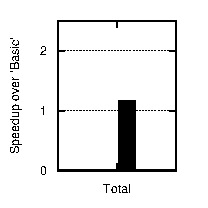
\includegraphics[width=\textwidth]{system/figures/copy-elision-comparison-total}
		\caption{Total time}
	\end{subfigure}
	~
	\begin{subfigure}{0.7\textwidth}
		\includegraphics[width=\textwidth]{system/figures/copy-elision-comparison}
		\caption{Individual query execution times}
	\end{subfigure}
	\caption{\textbf{Impact of template metaprogramming: Changes in total time and individual query times}}
	\label{fig-template-metaprogramming}
\end{figure}

Next, we toggle the use of the template metaprogramming (see Section~\ref{ssec:expression-eval}), using the SSB 100 scale factor dataset. Specifically, we change the compile time flag that determines whether the \texttt{ValueAccessor} is constructed by copying attributes (Basic) or by providing an indirection (Selection). The results for this experiment are shown in Figure~\ref{fig-template-metaprogramming}.

The overall performance impact of eliminating the copy during predicate evaluation is about 20\%. As with the previous experiment, the benefits are larger for the simpler Q1.X queries and lower for the other queries that tend to spend most of their time on join operations and in the pipelines in passing tuples between different join operations.

The result for this experiment with TPC-H show far smaller improvements (see Figure~\ref{fig:tpch-q10-waterfall} for a typical example), as the TPC-H queries spend a far smaller fraction on their overall time on expression evaluation (compared to the SSB queries).

\subsection{Impact of Optimization Techniques}
\label{sec:expt:optimization}

\begin{figure}[t]
	\centering 
	\begin{subfigure}[ht]{0.2\textwidth}
		\includegraphics[width=\textwidth]{system/figures/lip-ef-impact-total}
		\caption{Overall}
	\end{subfigure}
	~
	\begin{subfigure}[ht]{0.7\textwidth}
		\includegraphics[width=\textwidth]{system/figures/lip-ef-impact}
		\caption{Breakdown of speedup due to techniques}
	\end{subfigure}
	\caption{\textbf{Impact of Exact Filter and LIP using SSB at scale factor 100.}}
	\label{fig-lip-ef-impact}
\end{figure}

We described the novel optimization techniques in \Quickstep\ optimizer in Section~\ref{sec:query-opt}. In this experiment,
we measure the impact of these techniques individually, viz. LIP and join to semi-join transformation.

As with the previous two sections, we use the SSB 100 scale factor dataset. (The results for the TPC-H dataset is similar.)
Figure~\ref{fig-lip-ef-impact} shows the impact of these techniques over a baseline in which neither of these techniques are used. As shown in Figure~\ref{fig-lip-ef-impact}, these techniques together provide a nearly 2X speedup for the entire benchmark. The LIP and semi-join transformation techniques individually provide about 50\% and 20\% speedup
respectively. While some queries do see a slowdown due to the individual techniques, the application of both
techniques together always gives some speedup. In fact, of the 13 queries in the benchmark,
8 queries see at least a 50\% speedup and three queries see at least 2X speedup. The largest speedups
are in the most complex queries (group 4), where we see an overall speedup of more than 3X.

These results validate the usefulness of these techniques on typical workloads. Further, their simplicity of implementation and general applicability leads us to believe that these techniques should be more widely used in other database systems.

\subsection{Elasticity} \label{sec:expt:elasticity}

\begin{figure*}
	\centering
	\includegraphics[width=\textwidth]{system/figures/2-high-priority-queries.pdf}
	\caption{\textbf{Prioritized query execution. QX.Y(1) indicates that Query X.Y has a priority 1. Q4.2 and Q4.3 have higher priority (2) than the other queries (1).}}
	\label{fig-high-priority}
\end{figure*}

In this experiment, we evaluate \Quickstep's ability to quickly change the degree of inter-query parallelism, driven by the design of its work-order based scheduling approach (cf. Section~\ref{scheduler}). For this experiment, we use the 100 scale factor SSB dataset. The experiment starts by concurrently issuing the first 11 queries from the SSB benchmark (i.e. Q1.1 to Q4.1), against an instance of Quickstep that has just been spun up (i.e. it has an empty/cold database buffer pool).
All these queries are tagged with equal priority, so the Quickstep scheduler aims to provide an equal share of the resources to each of these queries. While the concurrent execution of these 11 queries is in progress, two high priority queries enter the system at two different time points. The results for this experiment are shown in Figure~\ref{fig-high-priority}.
In this figure, the y-axis shows the fraction of CPU resources that are used by each query, which is measured as the fraction of the overall CPU cycles utilized by the query.

Notice in Figure~\ref{fig-high-priority}, at around the 5 second mark when the high priority query Q4.2 arrives, the \Quickstep\ scheduler quickly stops scheduling work orders from the lower priority queries and allocates all the CPU resources to the high-priority query Q4.2.
As the execution of Q4.2 completes, other queries simply resume their execution.
%\reminder{We might want to increase some font sizes in this figure. Also, pick a color other than red for Q4.1.}

Another high priority query (Q4.3) enters the system at around 15 seconds.
Once again, the scheduler dedicates all the CPU resources to Q4.3 and pauses the lower priority queries.
At around 17 seconds, as the execution of query Q4.3 completes, the scheduler resumes the scheduling of work orders from all remaining active lower priority queries.

\begin{figure}
	\centering
	\includegraphics[width=0.6\columnwidth,height=4.2in]{system/figures/q31-progress.pdf}
	\caption{\small \textbf{Query progress status. Green nodes (0-5) indicate work that is completed, the yellow node (6) corresponds to operators whose work-orders are currently being executed, and the blue nodes (7-13) show the work that has yet to be started.}}
	\label{fig-query-progress}
\end{figure}

This experiment highlights two important features of the \Quickstep\ scheduler.
First, it can dynamically and quickly adapt its scheduling strategies. % in favor of the queries with higher priorities.
Second, the \Quickstep\ scheduler can naturally support query suspension (without requiring complex operator code such as~\cite{DavisonG94}), which is an important concern for managing resources in actual deployments.

\subsection{Built-in Query Progress Monitoring}\label{sec:progress-monitoring}
An interesting aspect of using a work-order based scheduler (described in Section~\ref{scheduler}) is that the state of the scheduler can easily be used to monitor the status of a query, without requiring any changes to the operator code. Thus, there is a generic in-built mechanism to monitor the progress of queries.

\Quickstep\ can output the progress of the query as viewed by the scheduler, and this information can be visualized. As an example, Figure~\ref{fig-query-progress} shows the progress of a query with three join operations, one aggregation, and one sort operation.


%% !TEX root = quickstep.tex

\section{Related Work} \label{related}
%The focus of this paper is on high performance in-memory analytics computing, and this paper narrows its focus to single machine NUMA settings. 
We have noted related work throughout this chapter, and we highlight some of the key areas of overlapping research here. 

There is tremendous interest in the area of main-memory databases and a number of systems have been developed, including~\cite{LarsonCFHMNPPRRS13, BonczKM08, RamanABCKKLLLLMMPSSSSZ13, hyper, XinRZFSS13, scuba, SparkSQL, vectorwise, FarberMLGMRD12, oracledbim}, 
%MonetDB~\cite{BonczZN05, BonczKM08, IdreosGNMMK12}, Blink~\cite{RamanSQRDKNS08}, Hyper~\cite{hyper}, Shark~\cite{XinRZFSS13}, Scuba~\cite{scuba}, SparkSQL~\cite{SparkSQL}, VectorWise~\cite{vectorwise}, SAP HANA~\cite{FarberMLGMRD12},  IBM DB2 BLU~\cite{RamanABCKKLLLLMMPSSSSZ13}, and Microsoft SQL Server~\cite{LarsonCFHMNPPRRS13}. 
While similar in motivation, our work employs a unique block-based architecture for storage and query processing, as well as fast query processing techniques for in-memory processing. The combination of these techniques not only leads to high performance, but also gives rise to interesting properties in this end-to-end system, such as elasticity (as shown in Section~\ref{sec:expt:elasticity}).

Our vectorized execution on blocks has similarity to the work on columnar execution methods, including recent proposals such as~\cite{SIMD-DBMS, RamanSQRDKNS08, JohnsonRSS08,WillhalmPBPZS09, WillhalmO0F13, bitweaving, AbadiMF06,  QiaoRRHL08, FengLKX15}. 
\Quickstep's template metaprogramming-based approach relies on compiler optimizations to make automatic use of SIMD instructions. Our method is complementary to run-time code generation (such as~\cite{JohnsonRSS08,WillhalmPBPZS09, WillhalmO0F13, AbadiMF06,  QiaoRRHL08, FengLKX15, archofadb, Neumann11, SparkSQL, PirkMZM16, NagelBV14, SIMD-DBMS, RamanSQRDKNS08}). Our template metaprogramming-based approach uses static (compile-time) generation of the appropriate code for processing tuples in each block. This approach eliminates the per-query run-time code generation cost, which can be expensive for short-running queries. An interesting direction for future work is to consider combining these two approaches.

% and we largely use BitWeaving as an index in this work, which falls under a broader class of efficient bit-based indexing/storage methods that are optimized for modern processors~\cite{FengL15, RamanSQRDKNS08, JohnsonRSS08, ONeilQ97, RinfretOO01, ChanI98, Wu99, Johnson99, Lamport75, WuOS06, Warren77,Barber12, FengLKX15}. We also use CSB+Tree~\cite{csbtree} as another indexing structure. 

%The implications of NUMA architectures for performance is well-known and has been a subject of significant research over the past few years. Some of the earliest work on query processing for NUMA includes the work by Bouganim et al.~\cite{BouganimFV97}. As NUMA architectures have become more main-stream, there has been a renewed interest in determining the impact of such change on analytical query processing, including~\cite{BlanasP13, BlanasLP11, LiPMRL13, BalkesenTAO15, BalkesenATO13,BarberLPRSACLS14,KieferSL13, KieferKSHML14, PsaroudakisSMSA15}.

The design of \Quickstep's storage blocks has similarities to the tablets in Google's BigTable~\cite{DBLP:conf/osdi/ChangDGHWBCFG06}.
However, tablets' primary purpose is to serve sorted key-value store applications whereas  \Quickstep's storage blocks adhere to a  relational data model allowing for optimization such as efficient expression evaluation (cf. Section~\ref{vectorization}).

Our use of a block-based storage design naturally leads to a block-based scheduling method for query processing, and this connection has been made by Chasseur et al.~\cite{quickstep-storage} and Leis et al.~\cite{LeisBK014}.
In this work, we build on these ideas. 
We also leverage these ideas to allow for desirable properties, such as dynamic elastic behavior (cf. Section~\ref{sec:expt:elasticity}).

Philosophically, the block-based scheduling that we use is similar to the MapReduce style query execution~\cite{mapreduce}. 
A key difference between the two approaches is that there is no notion of pipelining in the original MapReduce framework, however \Quickstep\ allows for pipelined parallelism.  Further, in Quickstep common data structures (e.g. an aggregate hash table) can be shared across different tasks that belong to the same operator.

The exact filters build on the rich history of semi-join optimization dating back at least to Bernstein and Chiu~\cite{Bernstein1981SemiJoin}. The LIP technique presented in Section~\ref{sec:lip} also draws on similar ideas, and is described in greater detail in~\cite{DBLP:journals/pvldb/ZhuPSP17}. 

Achieving \textit{robustness} in query processing is a goal for many database systems~\cite{graefe_et_al:DSP:2011:2984}.
\Quickstep\ uses the LIP technique to achieve robust performance for star-schema  queries. 
We formally define the notion of robustness and prove the robustness guarantees provided by Quickstep. 
VectorWise uses micro-adaptivity technique~\cite{DBLP:conf/sigmod/RaducanuBZ13} for robustness, but their focus is largely on simpler scan operations.

%There is a large body of work on auto-tuning parameters in a database engine (e.g.~\cite{ChaudhuriN07}) and self-managing databases (e.g.~\cite{ChaudhuriW00})

Overall, we articulate the growing need for the scaling-up approach, and present the design of \Quickstep\ that %employs fast kernels for data processing coupled with a flexible scheduler-based query processing architecture that 
is designed for a very high-level of intra-operator parallelism to address this need. We also present a set of related query processing and optimization methods. Collectively our methods achieve high performance on modern multi-core multi-socket machines for in-memory settings.

%with novel indexing and data normalization methods that are optimized for NUMA settings for in-memory analytical data processing environments. 

%% !TEX root = quickstep.tex

\section{Conclusions \& Future Work} \label{conclusions}
Compute and memory densities inside individual servers continues to grow at an astonishing pace. % and is likely poised to grow faster than the networks that connect nodes.
Thus, there is a clear need to complement the emphasis on ``scaling-out'' with an approach to ``scaling-up'' to exploit the full potential of parallelism that is packed inside individual servers. 
%In addition, in read-mostly data warehousing environments it is often common to use a distributed storage layer (e.g. HDFS or EBS) for fault-tolerance, which reduces the need to lean on distribution in the compute infrastructure to increase data availability. (We acknowledge that distributed execution does help query restart, but faster query execution also helps reduce the need for query restarts.) Many cloud infrastructure are getting built with a storage cloud component and a separate high-performance compute cloud component. These trends, arguably, point to a bigger emphasis on single-node compute performance especially when high single node performance can be used to reduce the overall total cost of processing queries. 


This paper has presented the design and implementation of \Quickstep\ that emphasizes a scaling-up approach. \Quickstep\ currently targets in-memory analytic workloads that run on servers with multiple processors, each with multiple cores. \Quickstep\ uses a novel independent block-based storage organization, a task-based method for executing queries,  a template metaprogramming mechanism to generate efficient code statically at compile-time, and optimizations for predicate push-down and join processing. 
We also present end-to-end evaluations comparing the performance of \Quickstep\ and a number of other contemporary systems. Our results show that \Quickstep\ delivers high performance, and in some cases is faster than some of the existing systems by over an order-of-magnitude. 

Aiming for higher performance is a never-ending goal, and there are a number of additional opportunities to achieve even higher performance in \Quickstep. Some of these opportunities include operator sharing, fusing operators in a pipeline, improvements in individual operator algorithms, dynamic code generation, and exploring the use of adaptive indexing/storage techniques. We plan on exploring these issues as part of future work. We also plan on building a distributed version of \Quickstep. 

%, and support a generic platform API that expands beyond SQL to include graph analytics, document stores and relational learning. Early prototypes show that these seemingly disparate analytic applications can be served using a platform that implements relational kernel operators~\cite{QuickFOIL, FanRP15, json-relational}. But, there are a number of issues related to optimization and execution that still need to be explored. 

%In this paper we presented the design, implementation, and evaluation of the current version of single-node \Quickstep. 
%, which uses a variety of novel techniques for data storage, indexing, and query processing for in-memory analytic query processing. 
%Key aspects of the \Quickstep\ architecture include the use of a novel block-based design for storage management and a corresponding  scheduler-based mechanism to break down a query into a sequence of work orders. This approach allows for a flexible way to adapt query execution mid-flight at run-time to use more hardware to speed up a query. \Quickstep\ also has in-built methods to effectively use NUMA hardware, which is becoming increasingly common in server configurations today. \Quickstep\ employs novel techniques such as BitWeaving to speed up scans, which are the workhorse of in-memory analytical database systems. \Quickstep\ also employs an aggressive schema-based denormalization method called WideTable to evaluate complex join queries using simple (BitWeaved) scans. Collectively, \Quickstep\ uses a set of new design points for in-memory analytical query processing, and in this paper we show how these aspects work in an end-to-end system. 

%There is a long list of next steps, including examining how to gracefully spill to disks/NVM storage, automatic physical schema tuning, building robust query optimization methods, and expanding to a distributed version of \Quickstep. % that works with the Hadoop YARN~\cite{yarn} framework. 


% ensure same length columns on last page (might need two sub-sequent latex runs)
%\balance

%\section{Acknowledgments}
%This work was supported in part by the National Science Foundation under grants  IIS-0963993, IIS-1110948, and IIS-1250886, and by gift donations from Google, Huawei and Pivotal. A project like \Quickstep\ would not have been possible without the support and contributions from many people over the years. In this regard, we would especially like to thank Shoban Chandrabose, Craig Chasseur, Julian Hyde, Rogers Jeffrey Leo John, Yinan Li, Adalbert Gerald Soosai Raj, Vaishnavi Sashikanth, Rathijit Sen, Gavin Sherry, Shivakumar Venkataraman and Qiang Zeng.  

%\balance
%\bibliographystyle{abbrv}
%\bibliography{refs} 
%\end{document}

%% !TEX root = scheduler.tex
\begin{abstract}
There is a growing need for in-memory database analytic services, especially in cloud settings. Concurrent query execution is common in such environments. 
A crucial deployment requirement is to employ a concurrent query execution scheduling framework that is flexible, precise, and adaptive to meet specified deployment goals. 
In addition, the framework must also aim to use all the underlying hardware resources effectively (for high performance and high cost efficiency). 
This paper focuses on the design and evaluation of such a scheduler framework. 
Our scheduler framework incorporates a design in which the scheduling policies are cleanly separated from the scheduling mechanisms, allowing the scheduler to support a variety of policies, such as fair and priority scheduling. 
The scheduler also contains a novel learning component to monitor and quickly adapt to changing resource requirements of concurrent queries. 
In addition, the scheduler easily incorporates a load controller to protect the system from thrashing in situations when resources are scarce/oversubscribed. 
We have implemented our scheduling framework in an in-memory database engine, and using this implementation we also demonstrate the effectiveness of our approach. 
Collectively, we present the design and implementation of a scheduling framework for in-memory database services on contemporary hardware in modern deployment settings.
\end{abstract}
% !TEX root = scheduler.tex
\chapter{Design and Implementation of Quickstep Scheduler}\label{chap:policy}

\section{Introduction}\label{sec:intro}
Concurrent queries are common in various settings, such as application stacks that issue multiple queries simultaneously and multi-tenant database-as-a-service environments~\cite{NarasayyaMSLSC15, NarasayyaDSCC13}.
%Scheduling concurrent queries is a classical problem in database systems, which involves co-ordinating their executions, while also managing the resources used for execution. 
There are several challenges associated with scheduling  concurrent execution of queries in such environments.

The first challenge is related to exploiting the large amount of hardware parallelism that is available inside modern servers, as it requires dealing with two key types of parallelism.
%efficiently utilizing the .  % considering the availability of large number of CPU cores. 
The first type is \textit{intra-query parallelism}. 
Modern database systems often use query execution methods that have a high intra-query parallelism~\cite{quickstep-storage,morsel,wang2016elastic}.
Concurrent query execution adds another layer of parallelism, i.e. \textit{inter-query parallelism}. 
%Modern servers offer lot of parallelism in terms of CPU cores. 
%Allocation of CPU resources to various tasks is a big challenge in this context. 

The second challenge is that workloads are often dynamic in nature. 
%Queries exhibit different characteristics in terms of their resource consumption behaviors and their arrival time is unpredictable.
For each query, its resource (e.g. CPU and memory) demands can vary over the life-span of the query. 
Furthermore, different queries can arrive and depart at any time. % points during the workload execution. 
Maintaining a  level of Quality of Service (QoS) with dynamic workloads is an important challenge for the database cloud vendor. 

%Query scheduler is key to the functioning of a database system, as it impacts factors such as performance, resource management and quality of service. 

To address these issues, we present a concurrent query execution scheduling framework for analytic in-memory database systems. 
%Formulating the design principles of the query scheduler requires understanding of its goals.
We cast the goals for the scheduler framework by relating it to a governance model, since
the framework \textit{governs} the use of resources for executing queries in the system. 
Next, we describe some goals for a governance model and translate them in the context of our framework.  

First, an ideal governance model should be \textit{transparent}, i.e. decisions should be taken based on the guiding principles and they should be clearly understandable.
In the context of scheduling, we can interpret this goal as requiring high level \textit{policies} that can govern the resource allocation among concurrent queries. 
This goal also highlights the need to \textit{separate mechanisms and policies}, a well-known system design principle~\cite{LampsonS76}.
The scheduler needs to provide an easy way to specify a variety of policies (e.g. priority-based or equal/fair allocation) that can be implemented with the underlying mechanisms.
%Such flexibility is cruicial for the database to be deployed in various scenarios. 
Ideally, the scheduler should adhere to the policy even if the query plan that it has been given has poor estimates for resource consumption.

Second, the governance model should be \textit{responsive} to dynamic situations. 
Thus, the scheduler must be reactive and auto-magically deal with changing conditions; e.g., the arrival of a high-priority query or an existing query taking far more resources than expected. 
A related goal for the scheduler is to \textit{control} and \textit{predictably deal} with resource thrashing.

Finally, the governance should be \textit{efficient} and \textit{effective}. 
Thus, the scheduler must work with the data processing kernels in the system to use the hardware resources effectively to realize high cost efficiency and high performance from the underlying deployment. 
In main-memory database deployments, one aspect of effective resource utilization requires using all the processing cores in the underlying server effectively. 

%We begin by listing a desired set of properties for a contemporary database scheduler. 
%First, the scheduler needs to provide an easy way to specify a variety of policies (e.g. priority-based or equal/fair allocation) to distribute the system resources among concurrent queries. 
%Such flexibility is required to allow the database service to be deployed in various scenarios. 
%Second, the scheduler must be reactive so that it can auto-magically deal with changing conditions (e.g. the arrival of a high-priority query or an existing query taking far more resources than expected). 
%Ideally the scheduler should be able to meet the policy goals even if the query plan that it has been given has poor estimates about projected resource consumption. 
%Third, the scheduler should have in-built mechanisms to deal with resource thrashing in a controlled and predictable way. 
%Finally, the scheduler must work with the data processing methods in the system to use all the hardware resources effectively to realize high cost efficiency and high performance from the deployment. 
%In main-memory database deployments, which is the focus of this paper, one aspect of effective resource utilization requires using all the processing cores in the underlying server box effectively. 
%
\textbf{Contributions:} We present the design of a scheduler framework that meets the above goals. 
We have implemented our scheduler framework in an open-source, in-memory database system, called \sys{}.
%The background of \sys{}, essential for understanding the scheduler design is presented
%in Section~\ref{sec:background}.
A distinguishing aspect of this paper compared to previous work
%from the related work (described in Section~\ref{sec:related}) 
is that we present a holistic scheduling framework to deal with both intra and inter query parallelism in a single scheduling algorithm. 
%and a clean separation of policy from mechanism allowing for the system to easily support a wide variety of policies. 
%as against a single scheduling algorithm. The framework is based on a query execution paradigm that uses smaller individual sub-tasks, which is found in many systems~\cite{morsel,wang2016elastic}.
Therefore, our framework is far more comprehensive and more broadly applicable than previous work.

Our framework employs a design that cleanly separates policies from mechanism. 
This design allows the scheduler to easily support a range of different policies, and enables the system to effectively use the underlying hardware resources. 
The clean separation also makes the system maintainable over time, and for the system to easily incorporate new policies. 
Thus, the system is \textit{extensible}. 
The key underlying unifying mechanism is a probability-based framework that continuously determines resource allocation among concurrent queries.
Our evaluation (see Section~\ref{sec:eval}) demonstrates that the scheduler can allocate resources precisely as per the policy specifications. 

The framework uses a novel learning module that learns about the resources consumed by concurrent queries, and uses a prediction model to predict future resource demands for \textit{each} active query. 
Thus, the scheduler does not require accurate predictions about resource consumption for each stage of each query from the query optimizer (though accurate predictions are welcome as they provide a better starting point to the learning component). 
The predictions from the learning module can then be used to react to changing workload and/or environment conditions to allow the scheduler to realize the desired policy. 
Our evaluations underline the crucial impact of the learning module in the enforcement of policies.
The scheduler has a built in load controller to automatically suspend and resume queries if there is a danger of thrashing.

Collectively, we present an end-to-end solution for managing concurrent query execution in complex modern in-memory database deployment environments.

The remainder of this paper is organized as follows: Section~\ref{sec:background} describes some preliminaries related to \sys{}. 
The architecture of the scheduler framework is described in Section~\ref{sec:design}. 
Section~\ref{sec:policy} describes the  formulation of the policies and the load control mechanisms.
Section~\ref{sec:eval} contains the experimental results. Related work is discussed in Section~\ref{sec:related}.
% !TEX root = scheduler.tex
\section{Background}\label{sec:background}
In this section we establish some prerequisites for the proposed Quickstep scheduler framework.
\sys{}~\cite{quickstep} is an open-source relational database engine 
% and SQL as its query language.  \sys{} 
designed to efficiently leverage contemporary hardware aspects such as large main memory, multi-core, and multi-socket server settings. 
%The system aims to deliver high performance in read-mostly data warehousing 
%environments.  
%While \sys{} targets environments in which datasets are mostly memory resident, it can also answer queries on datasets that do not fit in memory, as all the data are accessed via a buffer pool, that supports page evictions and replacements. 
% However,  the implementation of \sys{} largely targets settings in which the  entire 
%database fits in memory.

The control flow associated with query execution in \sys{} involves first parsing the query, and then optimizing the query using a cost-based query optimizer.
The optimized query plan is represented as a Directed Acyclic Graph (DAG) of relational operator primitives. 
%Currently, the system employs hash-based implementation for join and aggregate operators. 
The query plan DAG is then sent to a \textit{scheduler}, which is the focus of this paper. 
The scheduler runs as a separate thread and coordinates the execution of all queries. 
Apart from the scheduler, \sys{} has a pool of worker threads that carry out computations on the data. 

\sys{} uses a query execution paradigm (built using previously proposed approaches~\cite{qsstorage,morsel}), in which a query is executed as a sequence of \textit{work orders}. 
A work order operates on a data block, which is treated as a self-contained mini-database~\cite{qsstorage}.  (c.f.~\cite{supplement} for examples of work orders)
The computation that is required for each operator in a query plan is decomposed into a sequence of work orders. 
For example, a select operator produces as many work orders as there are blocks in the input table. 
\sys{}'s work order abstraction is tied with its storage management, which we describe in~\cite{supplement}.

% !TEX root = scheduler.tex
\section{Design of the Scheduler}\label{sec:design}
In this section, we present an overview of the components in the proposed \sys{} scheduler.

\subsection{Scheduler Architecture Overview}\label{ssec:scheduler-arch}
Figure~\ref{fig:scheduler-architecture} shows the architecture of the \sys{} scheduler.
We begin by describing the \textit{Query Manager}, that coordinates the progress of a single query in the system.
It maintains the query plan DAG, and a data structure called
the \textit{Work Order Container} to track all the work orders that are ready for
scheduling. 
Recall from Section~\ref{sec:background}, a description of the work carried out on a block of data is a \textit{work order}. 
The Query Manager generates schedulable work orders for each active operator node in the DAG. 
It also runs a rudimentary DAG traversal algorithm to determine when to activate nodes in the DAG. 
The algorithm is decribed in Appendix~\ref{apx:DAG-algo}.

\begin{figure}[]
	\centering
	\includegraphics[width=\columnwidth]{policy/figures/Scheduler-Architecture.pdf}
	\vspace*{-1.5em}
	\caption{Overview of the scheduler}
	\label{fig:scheduler-architecture}
	\vspace*{-1.5em}
\end{figure}

An important component of the system is the \textit{Policy Enforcer}.
It selects a query among all the concurrent queries, and schedules its work order for execution. 
This in essence is \textit{a scheduling decision}, and is taken based on a high-level policy provided to the system.
The policy is described in \textit{Policy Specifications}, which is an
abstraction that governs how resources are shared among concurrent queries. 

Policy Enforcer (PE) and various Query Managers (QM) communicate with each other as follows:
\textbf{QM}$\rightarrow$\textbf{PE}: Provides work orders that belong to the managed query for dispatching (to get executed).
\textbf{PE}$\rightarrow$\textbf{QM}: Upon completion of a work order, send a signal so that the QM can then decide if new nodes in the DAG can be activated, and if existing nodes can be marked as completed.
A detailed description of the Policy Enforcer is present in Section~\ref{ssec:policy-enforcer}. 

The Policy Enforcer contains a \textit{Load Controller} module, which is
responsible for ensuring that the system has enough resources to meet the
demands.
A new query in the system presents its resource requirements for its lifetime in the form of a \textit{Resource Map} to the Load Controller.
%The estimates provided in the Resource Map can come from the query optimizer or some other mechanism, which is irrelevant to the scheduler.
A sample resource map is presented in Appendix~\ref{apx:resource-map}.

The Load Controller determines the fate of a new query. 
If enough resources are available, it admits the query.
If the system risks thrashing due to the admission of the new query, it can take a number of decisions, including wait-listing the query or suspending older active queries to free up resources for the new query.
%The Policy Enforcer maintains queues for wait-listed and suspended queries as shown in Figure~\ref{fig:scheduler-architecture}.
We describe the Load Controller in Section~\ref{ssec:load-control-mech}.

The Policy Enforcer works with another module called the \textit{Learning Agent}. 
Execution statistics of completed work orders are passed from the Policy Enforcer to the Learning Agent.
This component uses a simple learning-based method to predict the time to 
complete future work orders using the execution times of finished work orders. 
Such predictions form the basis for the Policy Enforcer's decisions regarding scheduling the next set of work orders (cf. Section~\ref{ssec:learning} for details on Learning Agent).

%Work orders that are ready to execute are sent to a \textit{Foreman} module. 
%The Foreman simply acts as a link between the overall scheduler and a pool of 
%worker threads. 
The \textit{Foreman} module acts as a link between the Policy Enforcer and a pool of worker threads. 
It receives work orders that are ready for execution from the Policy Enforcer, and dispatches them to the worker threads. 
The Foreman can monitor the number of pending work orders for each worker, and 
use that information for load-balancing when dispatching work orders.
Upon completion of the execution of a work order, a worker sends execution statistics to the Foreman, which are further relayed to the Policy Enforcer.
New work orders due to pipelining are generated similarly (more details on pipelining can be found in Chapter~\ref{chap:pipeline}). 
We describe \sys{}'s thread model in the next section. 

\section{Thread Model}\label{sec:thread-model}
\sys{} currently runs as a single server process, with multiple user-space threads. 
There are two kinds of threads. 
There is one \textit{Scheduler} thread, and a pool of \textit{Worker} threads. 
All the components in the scheduler architecture except the worker thread pool run in the 
scheduler thread. 
In the current implementation, all threads are spun upfront when the database server 
process is instantiated, and stay alive until the server process terminates.

The threads use the same address space and use shared-memory semantics for data 
access. 
In fact the buffer pool is stored in shared memory, which is accessible by all the threads. 
Each worker thread is typically pinned to a CPU core. 
Such pinning avoids costs incurred when a thread migrates from one CPU core to another, which results in loss of data and instruction cache locality. 
We do not pin the scheduler thread, as its CPU utilization is low and it is not worth dedicating a CPU core for the scheduler thread.

Every worker thread receives a work order from the Foreman, executes it and then waits for the next work order.
In order to minimize worker's idle time, typically each worker is issued multiple work 
orders at any given time. 
%When a work order is sent to a worker thread, it executes the work order.
%the worker thread simply invokes %the appropriate \verb|execute()| method (described in~\ref{ssec:workorders}). 
Thread-safe queues are used to communicate between the threads.
The communication happens through light-weight messages from the sender to the receiver thread, which is internally implemented as placing a message object on the receiver's queue. 
A receiver reads messages from its queue. 
A thread (and its queue) is uniquely identified by its thread ID. 

The thread communication infrastructure also implements additional features like the ability to query the lengths of any queue in the system, and cancellation of an unread message. 

\subsection{Policy Enforcer}\label{ssec:policy-enforcer}
The Policy Enforcer assigns a probability value to each active query in the system. 
A scheduling decision is essentially \textit{probabilistic}, based on these probability values. 
The probability value assigned to a query indicates the likelihood of a work order from that query being scheduled. 
These probability values play a crucial role in the policy enforcement.
In Section~\ref{sec:policy}, we formally derive these probability values for different policies and also establish the relationship between probability values and the policy specifications.

An important information to determine such a probability value is an estimate about the run times of future work orders of the query.
This information provides the Policy Enforcer some idea about the future resource requirements of each query.
As the Policy Enforcer continuously monitors the resource allocation to different queries in the system, using these estimates, it can control the resource allocation with the goal of \textit{enforcing} the specified policy for resource sharing. 
%Using these estimates for the active queries, the Policy Enforcer can control the resource allocation to queries with the goal of \textit{enforcing} the specified policy for resource sharing. 
In the next section, we describe an estimation technique for the execution time of future work orders of a query.
\subsection{Learning Agent}\label{ssec:learning}
The Learning Agent module is responsible for predicting the execution times of the future work orders for a given query. 
It gathers the history of executed work orders of a query and applies a prediction model on such a history to estimate the execution time of a future work order.
This predicted execution time is used to compute the probability assigned to each query (cf. Section~\ref{sec:policy} for probability derivations).

An alternative to the Learning Agent could be a static method that assigns fixed probability values to active queries in the system. 
We now justify the need for the Learning Agent and highlight the limitations of the alternative mentioned above.
An illustrative example is presented in~\ref{apx:learning-motivation}.

The time per work order metric doesn't stay the same throughout a query's lifetime, for reasons such as variations in input data (e.g. skew), CPU characteristics of different relational operators (e.g. scan vs hash probe).
In each phase of the query, the time per work order is different.
As the query plan gets bigger, the number of phases in the plan increase.
In addition, different queries may be in different phases at a given point in time.
To make things more complicated, queries can enter or leave the system at any time.

Therefore, it is difficult to statically pick a proportion of CPU to allocate to the concurrent queries. 
Hence there is a need to ``learn'' the various phases in the query execution and dynamically change the proportion of resources that are allocated to each query, based on each query's phase.
Next, we study the methodology used by the Learning Agent.

\subsubsection{Learning Agent Methodology}
%The Learning Agent builds each query's \textit{execution profile} based 
%on the execution statistics of recently completed work orders for that query.
The Learning agent uses the execution times of previously executed work orders\\
($t_{w_{1}}, t_{w_{2}}, \ldots, t_{w_{k}}$) to predict the execution time of 
the next work order ($t_{w_{k+1}}$) for a given query.\footnote{In the beginning of a query execution, when enough information about work order execution times is not available, we use the default probabilities in the Policy Enforcer, instead of using default predicted times in the Learning Agent.}
Figure~\ref{fig:scheduler-cycle} shows the Learning Agent's interaction with other scheduler components.
%It receives the execution statistics of an  executed work order, and uses this information 
%to predict the execution time of the future work orders. 

\begin{figure}[]
	\centering
	\includegraphics[width=\linewidth]{policy/figures/Compact-SchedulerCycle.pdf}
	\vspace{-1.5em}
	\caption{Interactions among scheduler components}
	\label{fig:scheduler-cycle}
	\vspace{-1.5em}
\end{figure}

The set of previously executed work orders can belong to multiple relational operators in the query operator DAG. 
The Learning Agent stores the execution times of the work orders grouped by their source relational operator, e.g. the execution statistics of select work orders are maintained together and kept separate from those of aggregation work orders. 

%A prediction model is used to estimate the execution time of future work orders. 
\sys{}'s scheduler currently uses linear regression (specifically autoregression, which is a smaller class of linear regression) as the prediction model.
We chose linear regression as it is fast, accurate, and efficient w.r.t. the computational and the storage requirements of the model. 
%(New models can be easily added using an abstraction mechanism.) 
More details about our use of linear regression is described in~\ref{apx:linear-regression-usage}.

The problem of estimating the query execution time is well-studied, but requires complex methods~\cite{duggan2011performance, wu2013towards, li2012gslpi, 
chaudhuri2004estimating}. 
The Learning Agent does not require such methods. 
However, it can combine estimates from other methods with its own estimates.
%i.e. we try to predict the execution times of immediate work orders, as opposed  to a 
%global
%level estimation that may involve estimation of the progress of the query and prediction
%of query/workload completion times. The Learning Agent can be extended to use
%other techniques for the prediction, and is complimentary to other methods for
%estimation.

% !TEX root = scheduler.tex
\section{Policy Derivations and Load Controller Implementation}\label{sec:policy}
Our work focuses on two critical system resources for in-memory database deployments: CPU and memory. 
The policies treat CPU as a \textit{divisible resource}, and the policy specifications are defined in terms of relative CPU utilizations of queries or query classes.
The load controller implementation treats memory as a \textit{gating resource} and its goal is to avoid memory thrashing.
We justify the choice of resources for policies and load controller implementations in~\cite{supplement}.

%Next, we present the different policies that are currently implemented in \sys{} to highlight how one can encode policies to work with the probability-based scheduler. 
%As noted above the policies are specified in terms of the CPU resource. 
A policy specification consists of two parts: an inter-class specification (resource allocation policy across query classes), and an intra-class specification (resource allocations among queries within the same class). 
The default setting is uniform allocations for both intra and inter-class policies. 

In Section~\ref{ssec:load-control-mech}, we describe \sys{}'s load control mechanisms. 
The load controller takes admission control and query suspension decisions based on the memory resource.
%These load control mechanisms work in conjunction with the notion of query priority used in the policy implementations.

The scheduling policies, described below in Sections~\ref{ssec:fairness}, ~\ref{ssec:hpf}, and~\ref{ssec:proportional-priority} are subject to the decisions made by the load controller, i.e. the policies apply to the queries that are admitted by the load controller and have not been suspended. %by the load controller. 

%We note that our scheduler framework allows extending the policy implementations and the load control mechanisms to other resource types such as network and disk I/Os, but we defer such extensions to future work, primarily as our implementation is within the context of an in-memory database. 

The interpretations of various policies are presented in Table~\ref{table:policy-interpreatations}.
Note that for the Fair policy, there is only one class. 
For the priority-based policies, we assume that queries are tagged with priority (integer) values. 
%A higher integer implies higher priority. 
Next, we describe the probabilistic framework that we use to implement various policies
(cf. Table~\ref{table:policy-notations} for notations).

\begin{table}[t]
\centering
\begin{tabular}{|c|p{10cm}|}
\hline
\textbf{Policy} & \textbf{Interpretation} \\ \hline
Fair & In a given time interval, all active queries should get an equal proportion of the total CPU cycles across all the cores. \\ \hline%There is only one query class.
Highest Priority First (HPF) & 
%Queries are tagged with priorities and the priority values are ordered. 
Queries are executed in the order of their priority values; i.e. a higher priority query is preferred over a lower priority query for scheduling its work order. \\ \hline
Proportional Priority (PP) & 
%Each query is tagged with a priority value. 
The collective resources that are allocated to a query class (i.e. all queries with the same priority value) is proportional to the class' priority value based on a specified scale; e.g. (linear, exponential).
%in a two class policy, an exponential scale could be used to specify that the high priority class should be given 10 times the resources as the low priority class. 
\\ \hline
\end{tabular}
\caption{Interpretations of the policies implemented in \sys{}}
\label{table:policy-interpreatations}
\end{table}

\subsection{Fair Policy Implementation}\label{ssec:fairness}
\begin{table}[t]
	\centering
	\begin{tabular}{|p{0.1\columnwidth}|p{0.75\columnwidth}|}
		\hline
		\textbf{Symbol} & \textbf{Interpretation} \\ \hline
		$q_{i}$ & Query $i$ \\ \hline
		$pb_{i}$ & Probability assigned to $q_{i}$ \\ \hline
		$PV_{i}$ & The priority value for $q_{i}$ \\ \hline
		$t_{i}$ & Predicted work order execution time for $q_{i}$ \\ \hline
		$t_{PV_{i}}$ & Proportion of time allocated for the class with priority value $PV_{i}$ \\ \hline
		$prob_{PV_{i}}$ & Probability assigned to the class with priority value $PV_{i}$ \\ \hline
	\end{tabular}
	\caption{Description of notations}
	\label{table:policy-notations}
\end{table}

%\textbf{Policy Interpretation}: In a given time interval, all active queries should get an equal proportion of the total CPU cycles across all the cores.
%There is only one query class and the default (i.e. uniform) policy is used for intra-class queries. 
%Thus the collective CPU resource (i.e. all cores across all sockets) is to be shared \textit{equally} by all concurrent queries. 

We assume $k$ concurrent active queries: $q_{1}, q_{2}, \ldots q_{k}$. 
The probability $pb_{j}$ is computed as:
%\begin{displaymath}
%$pb_{j} = \frac{\frac{1}{t_{j}}}{\sum\limits_{i=1}^{k}\frac{1}{t_{i}}}$
%\end{displaymath}
$pb_{j} = (\frac{1}{t_{j}})/(\sum\limits_{i=1}^{k}\frac{1}{t_{i}})$

Observe that $pb_{j} \in (0, 1]$ and $\sum\limits_{j=1}^{k}pb_{j} = 1$. 
Therefore, the $pb_{j}$ values can be interpreted as probability values. 
As all the probability values are non-zero, every query has a non-zero chance of getting its work orders scheduled. 

Notice that $\forall i, j$ such that $1 \leq i, j \leq k$, 
%\begin{displaymath}
%\frac{pb_{i}}{pb_{j}} = \frac{t_{j}}{t_{i}}
%\end{displaymath}
$pb_{i}/pb_{j} = t_{j}/t_{i}$.
If $t_{i} > t_{j}$, it means that the work orders for query $q_{i}$ take longer time to execute than the work orders for query $q_{j}$. 
Thus, in a given time interval, fewer work orders of $q_{i}$ must be scheduled as compared to the query $q_{j}$. %, as depicted in Figure~\ref{fig:probability-explanation}.

The probability associated with a query determines the likelihood of the scheduler dispatching a work order for that query.
Thus, when $t_i > t_j$, $pb_j > pb_i$, i.e.  the probability for $q_{i}$ should be proportionally smaller than probability for $q_{j}$.

\subsection{Highest Priority First (HPF) Implementation}\label{ssec:hpf}
%\textbf{Policy Interpretation}: Queries are tagged with priorities and the priority values are ordered. 
%Queries are executed in the order of their priority values; i.e. a higher priority query is preferred over a lower priority query for scheduling its work order. 
%The intra-class policy is set to the default (i.e. fair to all the queries within the class)
%Queries in the same priority class are all treated equally, i.e. their resource allocation is identical.
%Each query $q_{i}$ is associated with a priority value $pv_{i}$, where $pv_{i}$ is a 
%positive integer. 
Let $\{PV_{1}, PV_{2}, \ldots, PV_{k}\}$ be the set of distinct priority values in the 
workload. 
A higher integer is assumed to imply higher importance/priority.
The scheduler first finds the highest priority value among all the currently active queries 
which is $PV_{max}$. % = max(PV_{1}, PV_{2}, \ldots, PV_{k})$. 
Next, a fair resource allocation strategy is used to allocate resources across all the active queries in that priority class. 

%Note that with the HPF policy, if higher priority queries keep arriving continually, then 
%lower priority queries could starve.

In some situations, the queries from the highest priority value may not have enough work to keep all the workers busy. 
In such cases, to maximize the utilization of the available CPU resources, the 
scheduler may explore queries from the lower priority values to schedule work orders.
\subsection{Proportional Priority (PP) Implementation}\label{ssec:proportional-priority}
%\textbf{Policy Interpretation}: Each query is tagged with a priority value.
%The collective resources that are allocated to a query class (i.e. all queries with the same priority value) is proportional to the class' priority value based on a specified scale; e.g. in a two class policy, an exponential scale could be used to specify that the high priority class should be given 10 times the resources as the low priority class. 
%The intra-class policy is set to the default (i.e. uniform).
Let $P = \{PV_{1}, PV_{2}, \ldots PV_{k}\}$ be the set of the distinct priority values 
in the workload. 
We assume a linear scale for the priority values. 
A higher integer is presumed to imply higher priority.

In a unit time, a class with priority value $PV_{i}$ should get resources for a time that is 
proportional to its priority value i.e. $PV_{i}$. 
Therefore, the class with priority $PV_{i}$ should be allocated resources for 
$t_{PV_{i}} = PV_{i}/\sum\limits_{j = 1}^{k}PV_{j}$ amount of time. 

We now estimate the number of work orders for priority class $PV_{i}$ that can be executed in its allotted time. 
For this task, we need an estimate for the execution time of a future work order from the class as a whole, referred to as $w_{PV_{i}}$ for the class with priority value $PV_{i}$.
Therefore, assuming $m$ queries in a given class and the individual estimates of 
work order execution times for queries with priority $PV_{i}$ are $t_{1}, t_{2}, \ldots, t_{m}$, then the predicted work order execution time for the class is $w_{PV_{i}} = \sum\limits_{j = 1}^{m}t_{j}/m$.
Therefore the estimated number of work orders executed for priority class $PV_{i}$ is
$n_{PV_{i}} = t_{PV_{i}} / w_{PV_{i}}$.

After determining $n_{PV_{1}}, n_{PV_{2}}, \ldots, n_{PV_{k}}$, which are the 
estimated number of work orders executed by all the priority classes in their allotted
time, computing probabilities for each class is straightforward.
The probability of priority class $PV_{i}$ is 
$prob_{PV_{i}} = n_{PV_{i}}/\sum\limits_{j = 1}^{k}n_{PV_{j}}$.
Next, we describe the load control mechanism. % in \sys{}.
\subsection{Load Control Mechanism}\label{ssec:load-control-mech}
Recall that the load control mechanism in \sys{} is designed to manage the availability of memory resource to the queries in the system.
This task requires continuous monitoring of memory consumption in the system.
The load controller component has two functions:
1) Determining if new queries are allowed to run (a.k.a. admission control).
2) Suspending queries if the system is in danger of thrashing.
We now explain how the load control mechanism realizes these two functions.

%In this section we describe some example load control mechanisms implemented in \sys{}.

Recall from Section~\ref{sec:design}, that a new query entering the system presents to the Load Controller its Resource Map that describes the query's estimated range of resource requirements.

We denote the minimum and maximum memory requirements for a given query as $m_{min}$ and $m_{max}$, the threshold for maximum memory consumption for the database as $M$ and the current total memory consumption as $m_{current}$. 
The term $m_{current}$ includes total memory occupied by various tables, run time data structures such as hash tables for joins and aggregations for all the queries in the system.

In the simplest case, when there is enough memory to admit the query, we have $m_{max} + m_{current} < M$. 
In this case, the load controller can let the query enter the system.

When memory is scarce, i.e. $m_{min}+m_{current}>M$, the query can not be admitted right away. 
Its admission depends on the system's policy (i.e. one of the policies described earlier).

If the system is realizing the fair policy, all queries have the same priority.
In this scenario, the load controller simply suspends the new query until enough memory becomes available, after which the query can be admitted.

For both priority-based policies, if the new query's priority is smaller than the minimum priority value in the system, then the load controller suspends the query. 
The suspended query can be admitted in the system when enough memory is available to admit it.
In the other case, the load controller finds queries from the lower priority values that have high memory footprints. 
It continues to suspend such queries from the lower priority levels (in decreasing order of memory footprints) until enough memory becomes available to admit the given query. 

%The load control mechanism can also be used continually to monitor the actual memory consumption of queries, and suspend existing queries if the actual memory consumption ($m_{current}$) approaches a pre-defined threshold limit.
%The decisions made by the load controller are logged, so that its actions can be viewed in a control dashboard.
% performs admission control for all the policies. In the future, the load controller can be made to monitor run--time memory allocations and with the help of the \sys{}'s buffer pool, control such allocations requested by queries in the system.
%or equal to the currently running queries in the system, the Load Controller may waitlist the query.
%However, if the new query has a higher priority than the currently running queries in the system, it can decide to make memory available for the query, so as to admit it.
%One possible way to free up the memory is by suspending existing queries in the system in decreasing order of their memory footprints, until there is enough memory available to let the new query in the system.
%The suspended queries can be reactivated when there are enough resources available to execute them. 
% !TEX root = scheduler.tex
\section{Evaluation}\label{sec:eval}
In this section, we present an evaluation of our scheduler. 
The goals of the experimental evaluation are as follows:
\begin{enumerate}
%\itemsep -0.1em
\item To check if the policy enforcement meets the expected criterion defined in 
the policy behavior. 
\item To illustrate the role of the learning component, we compare it against a policy implementation that doesn't use the learning-based feedback loop. 
%In this implementation, each query's probability is \textit{fixed} and \textit{statically determined}.
\item Examine the behavior of the learning-based scheduler in the presence of 
execution skew. 
\item To observe the behavior of the load controller component of the scheduler in extreme/overloaded scenarios.
\end{enumerate}

We use an instance from the Cloudlab~\cite{RicciEide:login14} platform for our evaluation,
which we described in Table~\ref{table:hardware}.

\begin{table}[bht]
\centering
\begin{tabular}{|p{3cm}|p{10cm}|}
\hline
\textbf{Parameter} & \textbf{Description} \\ \hline
Processor & 2 Intel Xeon Intel E5-2660 2.60 GHz (Haswell EP) processors\\ \hline
Cores & 10 per socket, 20 per socket with hyper-threading \\ \hline
Memory & 80 GB per NUMA socket, 160 GB total \\ \hline
Caches & L3: 25 MB, L2: 256 KB, L1 (both instruction and data): 32 KB \\ \hline
OS & Ubuntu 14.04.1 LTS \\ \hline
\end{tabular}
\caption{Evaluation Platform}
\label{table:hardware}
\end{table}
\subsection{\sys{} Specifications}
We now describe \sys{}'s configuration parameters that are  used in the experiments. 
All 40 threads in the system are used as worker threads.
%Each worker thread is pinned to a CPU core. 
%Such pinning prevents migration of a thread from one CPU core to another by the OS, which may incur cache misses and migration penalties.
%The scheduler thread is not pinned, as its CPU utilization is low and it is not worth dedicating a CPU core for the scheduler thread.
The buffer pool is configured with 80\% of the available system memory (126 GB). 
Memory for storage blocks, temporary tables, and hash tables is allocated from the buffer 
pool.
The block size for all the stored relations is 4 MB.
We preload the buffer pool before executing the queries, which means that the queries run on ``hot'' data. 

%To encode the priority information in a query, we modify \sys{}'s SQL parser.
%The example below shows a query with priority value as 2:
%\lstset{language=SQL, 
%	basicstyle=\ttfamily\footnotesize, 
%	showstringspaces=false,
%	keywordstyle=\color{cardinal}\bfseries, 
%	otherkeywords={WITH, PRIORITY},
%	emph=[1]{San,Diego}, emphstyle=[1]{\color{bondiblue}}}
%\begin{lstlisting}
%SELECT * FROM Employees WHERE age > 25 WITH PRIORITY 2;
%\end{lstlisting}
%\vspace{-1em}

\subsection{Experimental Workload}\label{ssec:workload}
For the evaluation, we use the Star Schema Benchmark (SSB)~\cite{ssb}. 
We justify the choice of SSB for our evaluation in Appendix~\ref{apx:ssb}.
%The dataset has 1 fact and 4 dimension tables. 
We use two variants of the SSB SF 100 dataset, namely uniform and skewed. 
%first, we generate uniform data in all the relations as per the  original benchmark specification~\cite{ssb}.
For the skewed dataset, the skew is introduced in the \textit{lo\_quantity} column of \textit{lineorder} table, as described by Rabl et al.~\cite{DBLP:conf/wosp/RablPJOO13}.
% with the values derived from a probability distribution function: $ P(X=x) = (0.3/1.3^{x})$.
%The range of values in \textit{lo\textunderscore quantity} column is $[1, 50]$. 
In the uniform dataset, each value in the domain [1, 50] is equally likely to appear in the \textit{lo\textunderscore quantity} column.
In the skewed dataset, 90\% values fall in the range [1, 10]. 

\subsection{Evaluation of Policies}\label{ssec:policy-eval}
In this section, we evaluate the policies that are currently implemented in the system.
%All the policies are specified in terms of the CPU resources. 
%With these experiments, 
Specifically, we verify if the actual CPU allocation among queries is in accordance with the policy specifications.
To calculate CPU utilization, we use a log of start and end times for all work orders. % and use this log to calculate the CPU utilization.

\subsubsection{Fair}
In this experiment, we execute all 13 queries from the SSB concurrently using the fair policy. 
As described in Table~\ref{table:policy-interpreatations}, the policy specification implies a fair sharing of CPU resources among concurrent queries.
The CPU utilization of the queries is depicted in Figure~\ref{fig:fair-cpu-util}.
As we can see, the CPU utilization of all the queries remains nearly equal to each other during the workload execution, despite queries belonging to different query classes with varying query complexities.

\begin{figure}[t]
	\centering
	\includegraphics[width=\columnwidth]{policy/figures/ssb-all-uniform-fair-cpu-util.pdf}
	\caption{CPU utilization of queries in fair policy}
	\label{fig:fair-cpu-util}
\end{figure}

Notice that the available CPU resources also get automatically distributed elastically among the active queries (e.g. at the 10 and 18 seconds marks) when a query finishes its execution. 
This elasticity behavior allows \sys{} to fully utilize the CPU resources at \textit{all} times.
\subsubsection{HPF}
Now we validate if the implementation matches the 
specification of the HPF (cf. Table~\ref{table:policy-interpreatations}) policy.
%which requires that when scheduling work orders, higher priority classes be 
%preferred over lower priority classes. 

%As before, we use all the 13 SSB queries for this experiment, 
All queries have the same priority value (1) except Q4.2 and Q4.3 which have a higher priority value (2). 
The execution begins with 11 queries having the same priority value. %, i.e. Q1.1 to Q4.1.
We inject Q4.2 in the system at around 5 seconds and Q4.3 at around 15 seconds.
Figure~\ref{fig:hpf-all} shows the CPU utilization of queries during the workload 
execution.

As the high priority queries arrive (at the 5 and 15 seconds marks), the existing queries pause their execution and the scheduler makes way for the higher priority query.
As the higher priority queries finish their execution (i.e. at the 7 and 16 seconds marks), the paused queries resume their execution.

The result of this experiment also demonstrates that \sys{}'s scheduler design naturally supports query suspension, which is an important concern in workload management. 

\begin{figure}[t]
	\centering
	\includegraphics[width=\columnwidth]{policy/figures/ssb-hpf-all.pdf}
	\caption{CPU utilization in HPF policy. Note that $a.b  (N)$ denotes a SSB query $a.b$ with priority $N$}
	\label{fig:hpf-all}
\end{figure}

\subsection{Proportional Priority Policy}
Now we examine the scheduler's behavior to the proportional priority policy %(cf. Section~\ref{ssec:proportional-priority}, 
in which the higher priority integer implies higher importance.
%In this policy, the CPU allocation to query classes should be in accordance to their priority values.

We pick two queries from each SSB class, and assign them a priority value. 
Our priority assignment reflects the complexity of the queries from the corresponding class. 
For instance, query class 1 has one join, class 2 has two joins and so on.
Recall that in our implementation a higher priority integer implies higher importance.
% cf. Section~\ref{ssec:proportional-priority}.

Figure~\ref{fig:pp-cpu-util} shows the CPU allocation among concurrent queries in the proportional priority policy.
We can see that a higher priority query gets proportionally higher share of CPU as 
compared to the lower priority queries.
When all queries from the priority class 8 finish their execution (11 seconds), the 
lower priority classes elastically increase their CPU utilization, so as to use all the CPU 
resources. 
Also note that among the queries belonging to the same class, the CPU utilization is 
nearly the same, as described in the policy specifications.

\begin{figure}[t]
	\centering
	\includegraphics[width=\columnwidth]{policy/figures/ssb-priority-uniform-2queries-perclass-cpu-util.pdf}
	\vspace{-2.5em}
	\caption{CPU allocation for proportional priority policy. Note that $a.b  (N)$ denotes a SSB query $a.b$ with priority $N$}
	\label{fig:pp-cpu-util}
	%	\vspace{-1em}
\end{figure}

\subsection{Impact of Learning on the Relative CPU Utilization}\label{ssec:learning-impact-cpu-util}
In this experiment, we compare the learning-based scheduler with a static non-learning based implementation (baseline).
We perform the comparison using fair policy, which should be the easiest policy for a static method to realize.

In the baseline, the probability assigned to each query remains fixed unless either a query is added or removed from the system.
If there are $N$ active concurrent queries in the system, each query gets a fixed probability $1/N$.
%In the proportional priority implementation, if the distinct priority levels are $p_1, p_2 
%\ldots p_k$, then priority $p_i$ gets a probability $\frac{p_i}{\sum\limits_{j = 
%0}^{k} 
%p_j} $.

We run $Q1.1$ and $Q4.1$ concurrently with the fair policy using both the learning and 
non-learning implementations.
Our metric for this experiment is the ratio of CPU utilizations of $Q4.1$ and $Q1.1$.
%The CPU utilization is calculated as explained in Section~\ref{ssec:policy-eval}.
As per the policy specifications, the CPU utilization for both queries in the fair policy 
should be equal. % to each other, which means the ideal ratio is 1.
Figure~\ref{fig:non-learning-comparison} shows the results of this experiment.
%We restrict the X-axis until both the queries are under execution. 

\begin{figure}[h]
	\centering
	\includegraphics[width=\columnwidth]{policy/figures/q1-q11-ratio-cpu-util.pdf}
	\caption{Ratio of CPU utilizations  $\frac{Q4.1}{Q1.1}$ for learning and non-learning 
		implementations}
	\label{fig:non-learning-comparison}
\end{figure}

Observe in Figure~\ref{fig:non-learning-comparison}, that the ratio in the non-learning implementation is closer to 2, meaning that the 
implementation is biased towards $Q4.1$. 
This behavior stems from the fact that the time per work order for $Q4.1$ is higher than $Q1.1$ (c.f. Figure~\ref{fig:q1.1-q4.1-time-per-wo} in Appendix~\ref{apx:learning-motivation}).
In contrast, the ratio of CPU utilizations in the learning implementation is nearly 1.
The learning based implementation can identify various phases in query execution for 
both the queries and adaptively change the CPU allocation as per the changing demands 
of the queries.
The non-learning implementation however fails to recognize the fluctuations in the CPU 
demands of queries and therefore does an unfair allocation of CPU resources.
%\subsubsection{Impact of Learning on Performance}\label{sssec:makespan-comparison}
%To gauge the impact of the learning on performance, we compare the makespan (i.e. the total execution time of the entire workload) in learning vs non-learning implementations.
%For this comparison, we again use the fair policy, as earlier. 
%%in the experiment described in Section~\ref{ssec:learning-impact}.
%Table~\ref{table:makespan-learning-vs-non-learning} describes the results of the experiments using two workloads using the makespans using learning and non-learning implementations.  
%
%We can observe that the overhead of learning is negligible, in fact it benefits the makespan of the SSB workload by around 11\%, as compared to the non-learning implementation. 
%This improvement is due to a ``fairer'' allocation of CPU resources to the queries in the learning implementation.
%Longer queries don't dominate the CPU resource consumption, because of which shorter queries can finish their execution sooner.
%, thereby freeing up CPU resources available for the longer queries, which in turn can finish execution faster.
%\begin{table}
%\centering
%\begin{tabular}{|c|l|l|}
%\hline
%\multirow{2}{*}{Workload} & \multicolumn{2}{c|}{Makespan (sec)} \\ \cline{2-3} 
% & Non learning & Learning \\ \hline
%Q1.1 and Q4.1 & 4.2 & 4.3 \\ \hline
%All SSB queries & 25.6 & 22.9 \\ \hline
%\end{tabular}
%\vspace{0.5em}
%  \caption{Makespan comparison of learning and non-learning implementation}
%  \label{table:makespan-learning-vs-non-learning}
%\end{table}
%We would like to stress that the primary goal of the learning implementation is to aid the scheduler to adhere to the high level policy. 
%These experiments %described in Section~\ref{ssec:learning-impact} and Section~\ref{sssec:makespan-comparison} 
%suggest that the learning implementation not only achieves its primary goal, but also helps improving the performance of the SSB workload. 
\subsection{Impact of Learning on Performance}\label{ssec:learning-impact-perf}
Here we analyze the impact of the learning-based approach on the performance of queries. 
We use two query streams, one for $Q1.1$ and another for $Q4.1$.
%We use the same setup as the previous experiment and begin the execution with 10 queries; with five instances each of $Q4.1$ and $Q1.1$ running concurrently. 
As one instance of $Q4.1$ finishes execution, another instance of $Q4.1$ enters the system (likewise for $Q1.1$).
We compare the throughput for both $Q4.1$ and $Q1.1$ using the learning implementation of the fair policy against its non-learning implementation.

%In real life workloads, there is often a mix of queries with different query execution times.
%Based on this setting, we assume two users of the database system issuing concurrent queries. 
%One user issues short running queries and another user issues longer running queries. 
%\sys{} runs both kinds of queries concurrently using fair policy. 

%We compare the throughput observed by both users in the learning-based fair policy with non-learning based fair policy implementation, at the end of \reminder{add time} minutes from the beginning of the workload execution. 
%The concurrent query execution begins with \reminder{add number} queries, \reminder{add number} from each user.
%As soon as a user is returned the result of a query, the same user issues the next query to \sys{}, which means the think time is 0. 

%Table~\ref{table:throughput-comparison} compares the throughput observed by the two users. 
%We can observe that the throughput for the user issuing longer queries is less impacted by the change in the policy implementation. 
%However, the user issuing shorter queries is highly benefited using a learning based implementation.
%The throughput is nearly \reminder{add number}X better in the learning implementation compared to the non-learning one. 
Figure~\ref{fig:q11-q41-throughput} plots the result of this experiment and shows the throughput for each query stream. 
The throughput for the $Q4.1$ stream is not affected considerably by the choice of the implementation. 
However using the learning implementation, the throughput of the $Q1.1$ stream improves significantly (up to 3x better than the non-learning implementation). 
The reasons for the improvement are as follows:
Following the result of the previous experiment (cf. Figure~\ref{fig:non-learning-comparison}), in the non-learning implementation, $Q1.1$ which has shorter work orders, is starved of CPU resources due to $Q4.1$, which has longer duration work orders. 
In the learning-based implementation however, the $Q1.1$ stream gets its fair share of CPU resource (more than that in the non-learning implementation). 
Therefore, $Q1.1$'s performance is improved, resulting in its increased throughput. 

This experiment highlights a two-fold impact of the learning module -- first, it plays a crucial role in the fair policy enforcement. 
Second, it improves performance of queries with lower CPU requirements when they are competing with queries with higher CPU demands, thereby also increasing overall system throughput with such mixed and diverse workloads. 

\subsection{Experiment with Skewed and Uniform Data}
In this experiment we test the learning capabilities of the \sys{} scheduler under the presence and absence of skew (skew description in Section~\ref{ssec:workload}).
We execute $Q1.1$ and $Q4.1$ on the skewed and uniform data.
We sort the skewed \textit{lineorder} table on the \textit{lo\_quantity} column, to amplify the impact of skew. 
For the predicate $lo\textunderscore quantity \leq 25$ on the skewed table, some blocks have high selectivity and others have low selectivity.

%	\subfigure[$Q1.1$]{\includegraphics[width=60mm]{policy/figures/q11-throughput.pdf}}
%	\subfigure[$Q4.1$]{\includegraphics[width=60mm]{policy/figures/q41-throughput.pdf}}

\begin{figure}[t]
	\centering
    \begin{subfigure}[b]{0.5\textwidth}
    	\includegraphics[width=\textwidth]{policy/figures/q11-throughput.pdf}
    \end{subfigure}%	
    ~
    \begin{subfigure}[b]{0.5\textwidth}
    	\includegraphics[width=\textwidth]{policy/figures/q41-throughput.pdf}
    \end{subfigure}%	   
	\caption{Impact of learning on the throughput}
	\label{fig:q11-q41-throughput}
\end{figure}
	
%To test the scheduler's ability to learn in the presence of skew, 
We compare the predicted work order times for each query with its observed work order times. % for the same query.
%For completion, we perform the same experiment on the skewed data and uniform data. 
%For this experiment, we use both the skewed and uniform data.
Figure~\ref{fig:pred-vs-observed-time-per-wo} presents the results of this experiment, with relative error of the prediction on the Y-axis and time on X-axis.
We can see that the relative error is very low in both the datasets for both queries. 
The execution of $Q1.1$ with skewed data takes longer than the uniform dataset.
The intermediate peaks in the relative error correspond to phase change in the execution plan. 
Note that the scheduler learns the phase changes quickly, and adjusts its estimates after each phase change. 

\begin{figure}[t]
	\centering
    \begin{subfigure}[b]{0.4\textheight}
    	\includegraphics[width=\textwidth]{policy/figures/q11-q41-prediction-accuracy-skew-data.pdf}
	\caption{Skewed dataset}    	
    \end{subfigure}%	
	~    
    \begin{subfigure}[b]{0.4\textheight}
    	\includegraphics[width=\textwidth]{policy/figures/q11-q41-prediction-accuracy-uniform-data.pdf}
	\caption{Uniform dataset}    	    	
    \end{subfigure}%	
	\caption{Comparison of predicted and observed time per work order}
	\label{fig:pred-vs-observed-time-per-wo}    
\end{figure}

\subsection{Load Controller}
In this experiment, we evaluate the effectiveness of the load controller.
We use two queries from each SSB query class.
The priority value assigned to a query reflects its complexity e.g. proportional to number of joins in the query plan.
We configure the load controller with the threshold for suspending queries as 56 GB. 
As the buffer pool size grows close to the threshold, the load control mechanism kicks in.

\begin{figure}[]
	\centering
	\includegraphics[width=0.6\textheight]{policy/figures/load-control-cpu-util.pdf}
	\caption{Load control: An SSB query $a.b$ with priority $N$ is denoted as $a.b (N)$}
	\label{fig:load-control-cpu-util}
\end{figure}

%Recall from Section~\ref{sec:background} that the 
\sys{}'s buffer pool stores the relational tables as well as hash tables used for joins and aggregations.
%The LRU-k based buffer pool implementation may evict cold pages if there is a need to make more memory available.
If the requested memory cannot be allocated, the load controller can suspend a query with the highest memory footprint. 
In the current implementation, we check for reactivating the suspended query upon every query completion. % using similar memory considerations as those described above. 
Figure~\ref{fig:load-control-cpu-util} shows the CPU utilization of the queries.

The execution begins with 6 queries.
At around 4 seconds, a higher priority query $Q4.1$ enters the system.
At this point $Q3.1$ has the highest memory footprint and the load controller
picks it as the victim for suspension.
We can observe in Figure~\ref{fig:load-control-cpu-util}, that from 4 to 11 seconds, the CPU utilization of $Q3.1$ is zero, reflecting its suspended state.
The same pattern is repeated as another high priority $Q4.2$ enters the system at around 12 seconds.
Once again $Q3.1$, that has the highest memory footprint, is suspended in order to allow $Q4.2$ to enter the system. 
Observe that in the 12 to 15 seconds time interval, $Q4.2$ gets executed and the suspended query $Q3.1$ doesn't utilize any CPU resource.

This experiment demonstrates the load control capabilities of the \sys{}
scheduler. 
It stresses an important feature of our scheduler, which integrates load-controller functionality. %closely with the resource allocation components, 
Thus, admission control and query suspension is handled holistically by the scheduler. 

% !TEX root = scheduler.tex
\section{Related Work}\label{sec:related}
%We now describe the related work on scheduling in database systems, operating systems (OS), and networks. %, and cluster computing. 

The \textit{work orders} abstraction is similar to other abstractions like \textit{morsels} in Hyper~\cite{morsel} and the \textit{segment-based parallelism}~\cite{wang2016elastic}. 
Such abstractions provide a means to achieve high intra-query, intra-operator data parallelism.
Hyper~\cite{morsel} uses a \textit{pull-based} scheduling approach i.e. workers \textit{pull} work (morsels) from a pool.
%Every worker thread continues to pull a morsel from a global pool, and executes it.
We use a \textit{push-based} model, where the scheduler controls the assignment of work to workers.
The pull-based dispatch model suffices for executing one query at a time. 
However, a push-based model can be simpler to implement sophisticated functionalities such as priority-based query scheduling, incorporating a flow control across multiple pipelines, (as shown in~\cite{wang2016elastic}), cache-conscious task scheduling.

The elastic pipelining implementation~\cite{wang2016elastic} uses a \textit{scalability vector} to vary the degree of parallelism of segments of the query plan.
The scalability vector tracks the query performance when number of cores are varied,  and it does not use any prediction technique.
Their objective is to maximize the performance of a single query executed on a cluster.
Our work focuses on resource sharing among concurrent queries, by enforcing policies using a learning-based approach. 
Additionally, we can accommodate estimates provided by other techniques.

There is related work~\cite{gupta2009fair} on ordering queries in a workload with different objectives such as fairness, effectiveness, efficiency and QoS. 
This work is complimentary to our scheduler design as it deals with ordering the queries \textit{before} they enter the system, where as we focus on scheduling \textit{admitted} queries. 
%\textit{Qshuffler}~\cite{ahmad2011interaction} is a query 
%scheduler for report generation workloads. 
%It clusters queries based on their interaction with each other and predicts the 
%performance of the mix using statistical methods.
%It does not preempt queries once they are scheduled, whereas \sys{}'s 
%scheduler uses fine grained control over query execution, allowing query suspension and resumption. 

%In business intelligence settings, workload management is an important challenge.
%Some techniques to manage workloads are based on QoS considerations. 
%Krompass et al.~\cite{krompass2007dynamic} identify and handle mis-behaving queries in a workload, and also propose an economic model for prioritizing and penalizing queries based on their service level agreements~\cite{krompass2006quality}.
%Such techniques can be combined with our scheduler. 
%For instance, our load-controller's action on a query that uses large amount of memory is to suspend it. 
%Alternate actions could be to re-prioritize, kill, or resubmit the query, as described in~\cite{krompass2007dynamic}.
%\sys{}'s prioritized query execution approach can be effective in  scenarios involving 
%SLAs. 

Several enterprise databases~\cite{res_gov, rm, DB2, teradatawm, gpdb, hpwm} offer
workload management solutions which %such as admission control capabilities, 
classify queries based on their estimated resource requirements, % (e.g. CPU, memory, I/O), 
encode resource allocation limits as resource pools and map workloads to such resource pools. 
While such estimation methods can be used to complement our approach, 
our scheduler can also work without such detailed estimation techniques. 
Prior research in this area~\cite{krompass2007dynamic, krompass2006quality} has focused on identifying misbehaving queries, prioritizing/penalizing queries to meet the service level objectives.
Our load controller can be complemented with such functionalities.

%Resource (particularly memory) management, is a crucial problem for database systems. 
%Prior work in this area~\cite{mehta1993dynamic, davison1995dynamic} has focused on dynamic memory allocation schemes.
%Mehta and Dewitt's~\cite{mehta1993dynamic} memory allocation scheme
%grouped queries by their estimated memory requirements, and allocated memory to different query classes. 
%Davison and Graefe introduced a resource brokering model~\cite{davison1995dynamic} to minimize query execution times with a constraint of fairness.
%These techniques are complimentary to our execution engine and can also be incorporated in our buffer manager. 

Predicting query performance is an active area of research. 
Earlier work~\cite{wu2013towards, wu2014uncertainty, duggan2011performance} includes analytical models based on the optimizer's cost models for both single query and multiple concurrent queries.
By design, our Learning Agent can incorporate such techniques, but can also function without them. 
More accurate work order execution time estimates can further improve adherence to the policy specifications.
%Wu et al.~\cite{wu2013towards, wu2014uncertainty} developed an analytical model using optimizer's cost model to estimate the CPU and I/O costs for individual query, and used a queueing model to estimate the execution times of concurrent queries in a workload.
%Duggan et al.~\cite{duggan2011performance} presented a model to estimate the performance impact of running concurrent queries.
%Our Learning Agent's prediction accuracy can benefit from such models, 
%Despite these advances in the area of execution time estimation, using 
%inaccurate estimates for achieving fairness may result into unfair schedules. 

%There is a significant interest in minimizing workload execution time by sharing 
%data and computations across queries.
%QPipe~\cite{harizopoulos2005qpipe} exploits common data and operations among 
%different queries. 
%CJoin~\cite{candea2009scalable} operator introduced by Candea et al. continuously 
%scans the fact table, applies predicates from different queries and routes the 
%results to individual queries.
%Zukowoski et al. proposed \textit{co-operative scans}~\cite{zukowski2007cooperative} 
%to share scan operations among concurrent queries. 
%%The sharing of scans reduces the number of I/O operations, increases the data 
%%sharing among concurrent queries thereby improving the latency of individual 
%%queries and the overall execution time. 
%SharedDB~\cite{giannikis2012shareddb} creates a single global query plan for a 
%workload to share computations across queries, thus making it suitable for high 
%throughput demanding environments. 
%These sharing approaches treat every query equally and it is not clear if they 
%can respect query priorities.
%Work and data sharing in \sys{} can be achieved by changing the way work orders are
%created, e.g. if multiple queries need to scan the same block, a single work order can
%be created for all of them. 
%In practice, we create separate work orders for different queries to keep the 
%execution simple.
%Additionally, many database systems \reminder{Can we use examples of Postgres, 
%Greenplum, SQL server, Oracle here?} still follow the \textit{query-at-a-time} 
%model.
%In such systems, our scheduler paves a way towards policy-driven execution
%of concurrent queries. 

Scheduling problem has also been studied in the OS and the networks community. 
%Kay and Lauder~\cite{kay1988fair} described \textit{Share}, a pioneering scheduler that ensured fairness for all the system users.
Our scheduler's probabilistic framework is inspired by the seminal lottery scheduling~\cite{lottery-scheduling} % by Waldspurger and Weihl,
in which different processes are assigned certain number of lottery tickets,
A lottery is conducted after every fixed time intervals and the winner process gets to execute in the next quantum. 

A key difference in lottery scheduling and our work is that the OS scheduling is usually preemptive. %, meaning that a process can be preempted after it uses its time slice. 
The OS maintains a process context that captures the state of the preempted process. 
\sys{}'s scheduling is non-preemptive, which means once a work order begins its execution on a CPU core, it continues to do so until completion.
Non-preemptive scheduling provides us an exemption from maintaining work order context (similar to process context), thereby simplifying the relational operator execution algorithms.

%\reminder{Removed OS refs}
%Meehan~\cite{meehean2011towards} analyzed various Linux CPU schedulers, %like O(1), CFS, and BFS. 
%showcased the issues of black box CPU scheduling and highlighted the need for increased transparency in CPU scheduling.
%%It achieves fairness by assigning equal proportion of time to the users and not 
%%to the individual processes that are running on the system. 
%%Pabla et al.~\cite{pabla2009completely} described how the Completely Fair Scheduler (CFS) strives to be fair to all the processes running in the Linux. 
%Peter et al.~\cite{peter2010design} proposed design principles for multi-core schedulers used in general purpose OS.
%Giceva et al.~\cite{giceva2013cod} advocated co-designing database and OS for their better integration.

\sys{}'s design philosophy is to make scheduling transparent and fine-grained, and to decouple mechanism from policies~\cite{LampsonS76} - a common theme found in the OS literature.

Deficit Round Robin (DRR)~\cite{shreedhar1996efficient} is a technique for network packet scheduling.
Our usage of work order execution time as a metric is similar DRR's usage of packet sizes. 
However DRR scheduling is inherently round robin based (with additional maintenance of quantum information), where as our scheduling is based on dynamic probabilities. 

Our scheduler is designed for an in-memory analytical database system. 
There are several such systems such as MonetDB~\cite{monetdb}, Spark SQL~\cite{spark-sql}.
%\reminder{Removed cluster scheduling refs}
%Cluster scheduling has received a wide attention recently.
%Isard et al.~\cite{isard2009quincy} encoded the problem of scheduling jobs on compute nodes in the cluster as a graph that captures the data-locality and fairness requirements of the jobs. 
%\textit{Tetris}~\cite{grandl2014multi} is a multi-resource cluster scheduler that packs tasks to machines based on their demands for different resources. 
%This paper focuses on a single node setting, however, such ideas may be interesting to purse in the distributed version of \sys{}, which is part of future work.
%In cluster scheduling, resource demands of tasks are usually well understood. 
%Therefore variations in the duration of task executions can be statically modelled 
%- e.g. changing the site of task execution, time for input data movement across 
%network, etc. 
%In contrast, predicting cardinality and time estimates in database systems is 
%still an active research area, therefore accurately modeling the entire query 
%execution before scheduling the query may be difficult.

%% !TEX root = scheduler.tex
\section{Conclusions and Future Work}\label{sec:conclusion}
%Query scheduling is an important problem and its importance is growing with the emerging trends in cloud databases.
We present a scheduler framework built on the principle of separation of policy and mechanism. 
It supports a wide-range of policies, even in dynamic workload settings and without requiring complex and accurate estimates from a query optimizer. 
The proposed framework is holistic as it also incorporates a load control mechanism. 
We have implemented our methods in an open-source in-memory database \sys{}, and also demonstrated the effectiveness of our approach.
%interesting properties such as resource allocation using fair and priority-based policies and in-built load control mechanisms. We demonstrate the effectiveness of the scheduler in enforcing the above policies with the SSB workload with uniform and skewed dataset. Our fine-grained task scheduling paradigm allows the scheduler to be reactive to unexpected situations such as arrival of a new high-priority query or sudden burst in resource demands.
There are many directions for future work, including extending the scheduler framework to the distributed version of \sys{}. %, and allowing more kinds of resources such as disk I/O and network and exploring more estimation techniques for our Learning Agent. 

%\include{intro/intro2}
%\include{background/background1}
%\include{synfinder/synfinder1}
%\include{rmony/rmony4}
%\include{falcon/falcon4}
%\include{smurf/smurf1}
%\include{opensource/opensource1}
%\include{discussion/discussion}
%\chapter{Conclusions and Future Work}
In this chapter, we discuss the lessons learnt, present our conclusions, and describe the future work.
Through this dissertation, we present the design and implementation of a query scheduler.
The goal of this scheduler is to efficiently execute queries in an in-memory environment while effectively exploiting the features provided by the modern hardware. 
A key contribution of this dissertation is to demonstrate that the scheduler is capable of playing an important role in the database system architecture.

\section{Lessons Learnt}
We now discuss the lessons learnt from this dissertation.

\subsection{Importance of Abstraction and Contracts}
A good abstraction is vital for developing a good system. 
The work order abstraction in Quickstep proved to be a boon for the query scheduler. 
It allowed us to construct different layers on top of simple operator execution, for which the  abstraction was created. 

There was a clarity of the contract between query optimizer and query scheduler: the query optimizer creates an immutable query plan (DAG of relational operators), which is then passed on to the query scheduler. 
Once the query scheduler starts to operate on the query plan, there is no going back to the optimizer. 

We designed the operators to be stateful and allowed the scheduler to access their state thereby getting more insights about the query execution progress.
The book-keeping related data structures are handled only by the scheduler thread, thus they need not be thread-safe, which helped simplify their design. 

\subsection{Importance of Query Scheduler for High Performance}
Achieving high performance is a never unending pursuit for database systems. 
Though the scheduler has a lot of power in terms of controlling resources and co-ordinating the query execution, it still needs support from other modules in the database system for high performance.
Query optimizer is a vital component of the system. 
Scheduling work for an optimal query plan is far more effective than that for a poor plan. 
Moreover, efficient implementation of relational operators is crucial to leverage the most from the hardware. 
Therefore, even though the scheduler is an important piece in the overall puzzle, it must work in tandem with other components in the system. 

\subsection{Importance of Measurement, Estimation, and Analysis}
Measuring and estimating performance in systems is highly important. 
Back-of-the-envelope calculations is a handy technique that can be useful to anticipate the effect of a technique or a change.
By doing such calculations, we may be able to save a lot of development effort. 

Our work on revisiting pipelining relied heavily on measuring performance and analyzing the impact of various techniques on performance. 
Putting the performance improvement of pipelining into perspective was only possible due to the emphasis on measurement.
We made lot of mistakes in attributing performance changes to wrong reasons and learnt some valuable lessons the hard way.

While dealing with many parameters, it is important to adhere to basic scientific principles, e.g, not changing two parameters simultaneously, while studying the effect of one.

%Between multi-core CPU and memory, which are the primary kinds of resources used by an in-memory database system; CPU is 
\section{Conclusions}
We now discuss the conclusions from individual chapters of this dissertation. 

In Chapter~\ref{chap:quickstep}, we present the design and implementation of the Quickstep database system. 
Quickstep has a unique block based storage management system, that supports variety of storage formats such as row store, column store along with support for compression. 
The query execution in Quickstep happens with the help of a task abstraction called work orders. 
The work orders abstraction connects storage management in Quickstep with the execution engine. 
Quickstep's query scheduler, which is the focus of this dissertation controls the execution of these work orders and thus manages query execution in the system. 
Through our experimental evaluation, we show that the intra-operator and inter-operator parallelism through the work orders abstraction speeds up the query execution in Quickstep.
The work order abstraction is instrumental for realizing intra-operator parallellism.
Comparison with other systems also show that Quickstep is faster than other systems, often by orders of magnitude. 

In Chapters~\ref{chap:policy} and Chapter~\ref{chap:pipeline}, we show that the scheduler can be used to meet multiple objectives.
In Chapter~\ref{chap:policy} we use the scheduler for the problem of resource governance.
We specifically target the problem of allocating resources such as CPU to concurrent queries according to well defined policies.
A key challenge in this problem is the fluctuation in the resource requirements of a query.
We target real time queries setting, in which queries could arrive at any time, thus it further complicates the problem.
Our solution uses a probabilistic framework for taking the scheduling decisions and thereby allocating resources to queries.
The probabilistic framework is backed by a learning agent, that monitors the resource consumption in the system and using learning techniques, predicts the resource requirements of queries in the near future.  
We form a close loop between scheduling decisions and the learning, where the learning agent monitors the system, predicts the future resource requirements and tweaks the probabilities. 
The adjusted probabilities result in change in the resource allocation, leading the system closer to meeting the high level policy goals.
Our experimental evaluation shows that Quickstep scheduler can meet the goals for a variety of policies including fair and priority-based. 

Chapter~\ref{chap:pipeline} uses the scheduler for the performance objective.
Here we analyze the role of pipelining in the in-memory settings. 
We cast pipelining as a schedule in which consumer tasks (or work orders) are interleaved with the producer tasks. 
We compare pipelining with a non-pipelining strategy in which the said interleaving is not present. 
The two strategies differ primarily in the eagerness of data processing by the consumer operator. 
We underscore the impact of various parameters such as number of threads, the size of blocks, and hardware prefetching on the relative performance of the two pipelining strategies. 
Our analysis (based on evaluation on TPC-H queries as well as an analytical model and microbenchmarking) shows that the relative gap between the two strategies is not as high as in the disk based settings. 
We highlight that the impact of pipelining on query processing should be considered holistically with all the parameters listed earlier. 
%One key contribution through our study is the importance of degree of parallelism in query performance. 
%Pipelining can provide superior performance in cases when operators in the pipeline have scalability issues (with increasing number of threads). 
%We present an algorithm that sequences the various pipelines in a query plan with the goal of maximizing query performance.  
%Our evaluation on TPC-H queries show that the algorithm often produces pipeline sequences with better performance than other pipeline sequences. 

\subsection{Future Work}
Our scheduling work leads to many interesting future work directions.
There is an ongoing effort to make Quickstep work efficiently on a distributed setup. 
The distributed setting offers some challenges which are not as relevant in the in-memory single node setting.
Locality of a work order execution is quite important in the distributed setting.
The penalty of a non-local execution involves high data movement cost over network, which can degrade query performance.

Load balancing is another important aspect that a distributed query scheduler has to worry about.
Overloading a node with work can throttle the query processing and may cause bottlenecks.
A subtle aspect in distributed query scheduling is that the control traffic (e.g. dispatching a work order, reeving work order completion feedback) may be expensive.
Therefore the scheduler may have to batch or aggregate control messages.

In the single node setting, the scheduler can play a big role in query processing on heterogeneous hardware.
An example of such system can be a server configured with an FPGA or a GPU.
If the scheduler can understand the strengths and weaknesses of each heterogeneous hardware component, it can route work orders to different components appropriately. 
A key challenge in this problem is to understand the memory access costs for different hardware components and thus estimating the cost of executing operations.	

%=======================================================================
% Bibliograph
%\bibliographystyle{plainnat}
\bibliographystyle{abbrv}
\addcontentsline{toc}{chapter}{Bibliography}
\begin{singlespace}
\bibliography{thesis}            % Make the bibliography
\end{singlespace}

%=======================================================================
% Appendices

%\begin{appendix}
%\section{Work Orders}\label{apx:workorders}
Work done for executing a query in \sys{} is split into multiple \textit{work 
orders}. %, as highlighted in Section~\ref{sec:background}. 
A work order contains all the information that is needed to process tuples in a given 
data block. 
A work order encapsulates the relational operator that is being applied, the relevant 
input relation(s), location of the input data block, any predicate(s) to be 
applied on the tuples in the input block, and descriptors to other run-time 
structures (such as hash tables).
%The input data location is specified in terms of a unique storage block ID, a join hash table identifier, or an aggregation hash table identifier. 
%In NUMA settings, a work order can also provide a preferred site for execution in the 
%form of a NUMA socket ID. 
%The scheduler then uses this information to make a 
%\textit{data-locality aware} scheduling decision. \reminder{Should we remove NUMA 
%because there are no experiments?}

Consider the following full table scan query to illustrate the work order concept:

\begin{lstlisting}[language=SQL, 
basicstyle=\ttfamily\small, 
showstringspaces=false,
keywordstyle=\color{cardinal}\bfseries, 
emph={San,Diego}, 
emphstyle=\color{bondiblue}\bfseries]
SELECT name FROM Employee WHERE city=`San Diego'
\end{lstlisting}	
\vspace{-0.4em}

The plan for this query has a simple \textit{selection} operator.  
For the selection operator, the number of work orders is same as the number of input blocks in the \verb+Employee+ table. 
Each selection work order contains the following information:
\begin{itemize}
\itemsep0.1em
\item {Relation: \verb+Employee+, attribute: \verb|name|}
\item {Predicate: \lstinline[language=SQL, 
                                   basicstyle=\ttfamily\small, 
                                   keywordstyle=\color{cardinal} \bfseries,
                                   emph={San,Diego}, 
                                   emphstyle=\color{bondiblue}\bfseries]|city=`San Diego'|}
\item {The unique ID of an input block from the \verb+Employee+ table}
\end{itemize}

The work orders for a join operation %(illustrated below) 
are slightly more complicated. 
For example, a \textit{probe work order},  contains the unique ID of the probe 
block, %(as described in Section~\ref{ssec:storage-manager}, a hash table is stored in a block in the buffer pool), build and probe relations, 
a pointer to the hash table, the projected attributes, and the join predicate.
Each operator algorithm (e.g. a scan or the build/probe phase of a hash-join) 
in the system has a C++ class that is derived from a root abstract base class that has a virtual method called \verb|execute()|.
Executing a work order simply involves calling the \verb|execute()| method 
on the appropriate operator algorithm C++ class object. 

\section{Storage Management in \sys{}}\label{apx:storage-manager}
Data organization in the \sys{} storage manager holds the key to intra-query 
parallelism~\cite{qsstorage}. 
Data in a relation are organized in the form of blocks. 
Each block holds a collection of tuples from a single table. 
A unique aspect of the storage organization in \sys{} is that blocks are considered to 
be independent and self-contained mini-databases. 
Thus, when creating an index, instead of creating a global index with 
``pointers'' to the tuples in blocks, the index fragments are stored within the blocks. 
Each block is internally organized into \textit{sub-blocks}. 
There is one \textit{tuple storage sub-block}, which could be in a row store or a 
column store format.
%\reminder{Should we add more formats like compressed column store etc?}. 
In addition, each block has one sub-block for each index created on the table. 
CSB+-tree~\cite{csb+-tree} and BitWeaving~\cite{bitweaving} 
indices are currently supported. 
The blocks are free to self-organize themselves and thus a given table may have blocks in different formats. 
For example, new blocks in a table may be in a row store format, while older blocks may 
be in a column store format.
%The block size is configurable %(in fact blocks in the same table can be of 
%%different sizes), %and the recommended block size is 4 MB.

This storage block design, as articulated earlier in~\cite{qsstorage} enables the query execution to be broken down into a set of independent tasks on each block. 
This is a crucial aspect that we leverage in the design of our scheduler. 

The storage manager also contains a \textit{buffer pool manager}. 
It organizes the memory as an array of slots, and overlays blocks on top of the slots (so block sizes are constrained to be a multiple of the underlying slot size). 
Memory allocations for data blocks for \textit{both} permanent and temporary tables are always made from a centralized buffer pool. 
In addition, all allocations for run-time data structures, such as hash tables are also made 
by the buffer pool. 
The buffer pool manager employs an LRU-2 replacement policy. 
Thus, it is possible for a hash table to get evicted to disk, if it has become ``cold''; e.g. if it belongs to a suspended query.

\section{DAG Traversal Algorithm}\label{apx:DAG-algo}
The Query Manager is presented with a DAG for each query, where each
node in the DAG represents a relational operator primitive.
The edges in the DAG are annotated with whether the 
\textit{consumer} operator is blocked on the output produced 
by the \textit{producer} operator, or whether data pipelining is
allowed between two adjacent operators. 

Consider a sample join query and its DAG showed in Figure~\ref{fig:dag}.
The solid arrows in the DAG correspond to ``blocking'' dependencies,
and the dashed arrows indicate pipeline-able/non-blocking dependencies. 
To execute this query we need to select tuples from the \verb+ddate+ 
table, stream them to a hash table, which can then be probed by tuples that are 
created by the selection operator on the \verb+lineorder+ table. %(i.e. match the predicate on that table). 
The output of the probe hash operation can be sent to the print operator, which
displays the result. % tuples. 
Note that the ``drop hash'' operator is used to drop the hash table, but only 
after the ``probe hash'' operation is complete. 
Similarly, the other drop operators indicate when intermediate data can be deleted. 

\begin{algorithm}
	\caption{DAG Traversal}
	\begin{algorithmic}[1]
		\State G = \{V, E\}
		\State activeEdges = \{e $\in$ E $|$ e.isNotPipelineBreaking()\}
		\label{alg:pipelining}
		\State inactiveEdges = \{e $\in$ E $|$ e.isPipelineBreaking()\}
		\State completedNodes = \{\}
		
		\For {v $\in$ V}:
			\If {v.allIncomingEdgesActive()}
				\State v.active = True
			\Else
				\State v.active = False
			\EndIf
		\EndFor
		
		\While {completedNodes.size() $<$ V.size()}
		\For {v $\in$ V -- completedNodes}
		\If {v.allIncomingEdgesActive()}
			\State v.active = True \label{alg:depMet}
		\EndIf
		\If {v.active}
		\State v.getAllNewWorkOrders() \label{alg:getWork}
		\If {v.finishedGeneratingWorkOrders()} \label{alg:finishGenWork}
		\State completedNodes.add(v) \label{alg:nodeComplete}
		\For {outEdge $\in$ v.outgoingEdges()}
		\State activeEdges.add(outEdge)\label{alg:outEdgesActive}
		\EndFor
		\EndIf
		\EndIf
		\EndFor	
		\EndWhile
	\end{algorithmic}
	\label{alg:dag-traversal}
\end{algorithm}

\begin{figure}[]
	\centering
	\includegraphics[width=\columnwidth]{policy/figures/QueryPlan.pdf}
	\vspace*{-2em}
	\caption{A join query and its DAG}
	\label{fig:dag}
%	\vspace*{-1.5em}
\end{figure}

The Query Manager uses a DAG Traversal algorithm (cf. Algorithm~\ref{alg:dag-traversal}) to process the DAG, which essentially is an iterative graph traversal method. 
The algorithm simply finds nodes in the DAG that have all their dependencies met, and marks such nodes as ``active'' (line~\ref{alg:depMet}).
Work orders are requested and scheduled for all active nodes (line~\ref{alg:getWork}), and 
the completion of work orders is monitored. 
Operators are stateful and they produce work orders when they have the necessary data.
The work order generation stops (line~\ref{alg:finishGenWork}) when the operators no longer have any input to produce additional work orders.
When no more work orders can be generated for a node, that node is marked as 
``completed'' (line~\ref{alg:nodeComplete}). 
When a node is marked as completed, all outgoing blocking edges (the solid lines 
in Figure~\ref{fig:dag}) are ``activated'' (line~\ref{alg:outEdgesActive}). 
Pipelining is achieved as all non-blocking edges (dotted lines in 
Figure~\ref{fig:dag}) are marked as active upfront (line~\ref{alg:pipelining}).
The query is deemed as completed when all nodes are marked as ``completed.''

% Note(harshad) - The DAG traversal example seems to be taking lots of space and can be omitted, as it diverts the attention away from the meat of the paper. 
%\subsubsection{DAG Traversal Example}\label{sssec:dag-traversal-example}
%To illustrate the execution of the scheduler algorithm, consider the 
%DAG shown in Figure~\ref{fig:dag}.
%Initially, only the two selection relational operators (shown in the DAG using
%the symbol $\sigma$) are \textit{schedulable}.\footnote{Initially, the print 
%operator is \textit{active} too, but as there's no input available, it can't
%produce any work order.}
%So, the Query Manager generates work orders for these operators. 
%In this case, there is one work order for each input block in each of the two
%input relations.\footnote{To avoid both select operators from being co-scheduled
%concurrently, a dependency link can be created between these two operators.
%Thus, work on the select operator on the $\mathtt{lineorder}$ table is started
%only after the select operator on the $\mathtt{ddate}$ table has completed. 
%Such decisions are made by the optimizer.}
%
%The Foreman assigns these work orders to the available worker threads. 
%The worker threads execute the operations specified in the work orders. 
%Note that given the independent block design (see Section~\ref{ssec:storage-manager}) 
%it is possible that two work orders on the same table may invoke different code paths. 
%For example one block on the \verb+ddate+ table may have an index sub-block on 
%the \verb+d_year+ attribute, and this index may be chosen to evaluate the tuples 
%in that block. 
%Another block on that same \verb+ddate+ table may not have any indices, and so 
%the selection operation for tuples in that second sub-block may resort to a simple scan. 
%In addition, the operator algorithm may choose to make a local decision on which 
%access plan to use. 
%So, e.g. even if each data block in the \verb+ddate+ table has an index 
%of the \verb+d_year+ attribute some work orders may use the index and others may 
%not. (The optimization algorithm for making these local decisions is beyond the 
%scope of this paper.)
%Essentially, the scheduler is largely oblivious to how the work orders are executed 
%and there is no global recipe that is imposed on the work orders that correspond 
%to a node in the DAG.
%
%Work orders may produce output data that are stored in blocks in the buffer pool. 
%In the case of the query in Figure~\ref{fig:dag}, the selection work orders on the \verb+ddate+
%table insert the selected tuples into data blocks that correspond to a new 
%temporary table. 
%%(the execution of the work orders is vectorized for efficiency). 
%These data blocks are pipelined to the next stage.\footnote{There is a 
%mechanism to allow multiple concurrent work orders from the same
%operator in the DAG to insert into a common output/temporary data
%block to avoid block internal fragmentation, and to facilitate early 
%pipelining. We omit these details.}
%In other words, as soon as there is a full block of tuples from applying the 
%selection operator on the \verb|ddate| table, a work order is created for the 
%\textit{build hash} operator. (Notice that the edge connecting the selection
%operator and the build hash operator permits data pipelining.)
%
%To begin the probe phase of the hash join, the building of the hash table must be 
%complete, as there is a pipeline-breaking dependency between the probe operator 
%and the build operator. 
%Thus, the DAG traversal algorithm only marks the probe hash operator node as 
%active when the build hash operator has completed. 
%Results from probing the hash table can be immediately pipelined to the print 
%operator.
%The drop operators ensure that intermediate data is dropped before the query is 
%deemed to have completed. 

\section{Resource Map Discussion}\label{apx:resource-map}
An example Resource Map of an incoming query to the system is shown below:
\begin{lstlisting}[language=python, 
								   basicstyle=\ttfamily\small, 
								   showstringspaces=false,
								   keywordstyle=\color{bondiblue}\bfseries, 
								   emph={CPU, Memory}, 
								   emphstyle=\color{cardinal}\bfseries]
CPU:    {min: 1 Core, max: 20 Cores}
Memory: {min: 20 MB,  max: 100 MB}
\end{lstlisting}

This Resource Map states that the query can use 1 to 20 cores (i.e. specifies the range of intra-operator parallelism) and is estimated to require a minimum of 20 MB of memory to run, and an estimated 100 MB of memory in the worst case.

In \sys{}, the query optimizer provides the estimated memory requirements for a given query.
Other methods can also be used, such as inferring the estimated resources from the previous runs of the query or other statistical analyses.
The scheduler is agnostic to how these estimates are calculated.

\section{Pipelining in \sys{}}\label{apx:pipelining}
During a work order (presumably belonging to a producer relational operator in a pipeline) execution, output data may be created (in blocks in the buffer pool). 
When an output data block is filled, the worker thread sends a ``block filled'' message to the corresponding query's manager via the following channel: Worker $\rightarrow$ Foreman $\rightarrow$ Policy Enforcer $\rightarrow$ Query Manager.
The Query Manager may then create a new work order (for a consumer relational operator in the pipeline) based on this information;
e.g. if this block should be pipelined to another operator in the query plan.

Note that pipelining in \sys{} works on a block-basis, instead of the traditional tuple-basis.

\section{Thread Model}\label{apx:thread}
\sys{} currently runs as a single server process, with multiple user-space threads. 
There are two kinds of threads. 
There is one \textit{Scheduler} thread, and a pool of \textit{Worker} threads. 
All the components in the scheduler architecture except the worker thread pool run in the 
scheduler thread. 
In the current implementation, all threads are spun upfront when the database server 
process is instantiated, and stay alive until the server process terminates.

The threads use the same address space and use shared-memory semantics for data 
access. 
In fact the buffer pool is stored in shared memory, which is accessible by all the threads. 
Each worker thread is typically pinned to a CPU core. 
Such pinning avoids costs incurred when a thread migrates from one CPU core to another, which results in loss of data and instruction cache locality. 
We do not pin the scheduler thread, as its CPU utilization is low and it is not worth dedicating a CPU core for the scheduler thread.

Every worker thread receives a work order from the Foreman, executes it and then waits for the next work order.
In order to minimize worker's idle time, typically each worker is issued multiple work 
orders at any given time. 
%When a work order is sent to a worker thread, it executes the work order.
 %the worker thread simply invokes %the appropriate \verb|execute()| method (described in~\ref{ssec:workorders}). 
Thread-safe queues are used to communicate between the threads.
The communication happens through light-weight messages from the sender to the receiver thread, which is internally implemented as placing a message object on the receiver's queue. 
A receiver reads messages from its queue. 
A thread (and its queue) is uniquely identified by its thread ID. 

The thread communication infrastructure also implements additional features 
like the ability to query the lengths of any queue in the system, and cancellation 
of an unread message. 
For simplicity, we omit discussion of these aspects. 
\section{Motivation for the Learning Agent Module}\label{apx:learning-motivation}
One might question the need of the Learning Agent and instead consider assigning a fixed probability value to each query (say $1/N$, with $N$ queries in the fair policy).
In the following section, we address this issue. 
A motivational example for the learning agent is described in Appendix~\ref{apx:learning-motivation}.

We perform an experiment, where the goal is to analyze the patterns in work order execution times of two queries. 
The dataset used for the experiment comes from the Star Schema Benchmark (SSB)~\cite{ssb} 
at a scale factor of 100. %(c.f. Section~\ref{ssec:workload} for benchmark details).
We pick two SSB queries $Q1.1$ and $Q4.1$, and execute them on a machine with 40 CPU cores. 
$Q1.1$ has a single join operation and $Q4.1$ has four join operations.
Figure~\ref{fig:q1.1-q4.1-time-per-wo} shows the observed average time per work order for both queries.
We now describe the trends in time per work order for the queries.

We can observe $Q1.1$'s execution pattern denoted by the dashed line in Figure~\ref{fig:q1.1-q4.1-time-per-wo}. 
The time per work order remains fairly stable (barring some intermittent fluctuations) from the beginning until 1.8 s.
This phase corresponds to the selection operation in $Q1.1$ which evaluates predicates on the \textit{lineorder} (fact) table.
A small bump in time per work order can be observed at the 1.8 s mark, when the probe phase of $Q1.1$ begins and continues until 2 s.
Towards the end of the execution of $Q1.1$, (2.2 s) there is a spike in time per work order when the query enters the aggregation phase. 
The output of the hash join is fed to the aggregation operation. 
The results of aggregation are stored in per-thread private hash tables, which are later merged to produce the final output.

\begin{figure}[h]
	\centering
	\includegraphics[width=\columnwidth]{policy/figures/q11-q41-time-per-wo.pdf}
	\vspace{-2.5em}
	\caption{Time per work order for Q1.1 and Q4.1}
	\label{fig:q1.1-q4.1-time-per-wo}
%	\vspace{-2em}
\end{figure}

Now we analyze the execution pattern for $Q4.1$ which has 4 join operations. 
This query is more complex than $Q1.1$.% which has a single join.
%Due to the more complex nature of the query, 
Therefore, the execution pattern of $Q4.1$ exhibits more phases, with different times per work order as compared to $Q1.1$.
Various small phases before the 0.5 s mark correspond to the selection predicates that are applied to the dimension tables. (Note that in $Q4.1$ there is no selection filter on the \textit{lineorder} table).
The selections on dimension tables get executed quickly.
The longer phases denote the different probe hash table operations in the query.
Towards the end, similar to $Q1.1$, there is a spike in the execution time per work order which correspond to the aggregation phase.

It is clear that the work order execution times for both queries are different, and the difference between them changes over time. 
If the scheduler assigns the same probability to both queries (i.e. 0.5), it is equally likely to schedule a work order from either of them. 
As a result, the queries will have different CPU utilization times in a given epoch, thus resulting in an unfair CPU allocation. 
In order to be consistently fair in allocating CPU resources to the queries, we should continuously observe the work order execution times of queries and adjust the CPU allocation accordingly. 

\section{Usage of Linear Regression in Learning Agent}\label{apx:linear-regression-usage}
The Learning Agent uses linear regression for predicting the execution time of the future work orders.
To lower the CPU and memory overhead of the model, we limit the amount of execution statistics stored in the Learning Agent.
We discard records beyond a certain time window. 
When all the work orders of an operator finish execution, we remove its records completely. 
In a query, if multiple relational operators are active, linear regression combines the statistics of all active operators and predicts a single value for the next work order execution time.

\section{Resource Choices for Policy Implementations and Load Controller Implementations}\label{apx:resource-discussion}
In the current implementation of \sys{}, we have focused on two key types of resource in the in-memory deployment scenarios -- CPU and memory. 
Both these resources have different resource characteristics, which we outline below.

First, consider the CPU resource. 
On modern commodity servers there are often tens of CPU cores per socket, and the aggregate number of cycles available per unit time (e.g. a millisecond) across all the cores is very large. 
Further, an implication of \sys{}'s fine-grained task allocation and execution paradigm is that the CPU resource can be easily shared at a fine time-granularity. 
Several work orders, each from different query can be executed concurrently on different CPU cores, and each query may execute thousands or millions or even more number of work orders. 
Thus, in practical terms, the CPU resource can be viewed as a nearly infinitely divisible resource across concurrent queries. 
In addition, overall system utilization is often measured in terms of the CPU utilization. Combining all these factors, specifying a policy  in terms of the CPU utilization is natural, and intuitive for a user to understand the policy. 
For example, saying that a fair policy equally distributes the CPU resource across all (admitted) concurrent queries is simple to understand and reason. 

Memory, on the other hand, is a resource that is allocated by queries in larger granular chunks. 
Active queries can have varying memory footprints (and the footprint for a query can change over the course of its execution). 
Thus, memory as a resource is more naturally viewed as a ``gating'' resource. 
Therefore, it is natural to use it in the load controller to determine if a query can be admitted based on its requested memory size. 
Actual memory consumption for queries can also be easily monitored, and when needed queries can be suspended if memory resource needs to be freed up (for some other query, perhaps with a higher priority). 

\section{Applicability of SSB for our evaluation}\label{apx:ssb}
The SSB is based on the TPC-H benchmark, and is designed to measure the query performance when %database systems in support of classical 
the data warehouse uses the popular Kimball~\cite{Kimball} approach. 
At a scale factor of X, the benchmark corresponds to about X GB of data in the 
corresponding TPC-H warehouse.
The SSB benchmark has 13 queries, divided in four categories. 
Each query is identified as \textbf{qX.Y}, where $X$ is the class and $Y$ is the query 
number within the class.
There are four query classes, i.e. $1\leq X\leq4$. 
The first and second classes have three queries each, the third class has four queries, and 
the fourth class has three queries.
The queries in each category are similar with respect to aspects such as the 
number of joins in the query, the relations being joined, the filter and aggregation 
attributes. 
The grouping of queries in various classes makes this benchmark suitable for our 
experiments, as it provides a way of assigning priorities to the queries based on their class. 

\section{Evaluation of Proportional Priority Policy}\label{apx:pp-policy-exp}
Now we examine the scheduler's behavior to the proportional priority policy %(cf. Section~\ref{ssec:proportional-priority}, 
in which the higher priority integer implies higher importance.
%In this policy, the CPU allocation to query classes should be in accordance to their priority values.

We pick two queries from each SSB class, and assign them a priority value. 
Our priority assignment reflects the complexity of the queries from the corresponding class. 
For instance, query class 1 has one join, class 2 has two joins and so on.
Recall that in our implementation a higher priority integer implies higher importance.
% cf. Section~\ref{ssec:proportional-priority}.

Figure~\ref{fig:pp-cpu-util} shows the CPU allocation among concurrent queries in the proportional priority policy.
We can see that a higher priority query gets proportionally higher share of CPU as 
compared to the lower priority queries.
When all queries from the priority class 8 finish their execution (11 seconds), the 
lower priority classes elastically increase their CPU utilization, so as to use all the CPU 
resources. 
Also note that among the queries belonging to the same class, the CPU utilization is 
nearly the same, as described in the policy specifications.

\begin{figure}[t]
	\centering
	\includegraphics[width=\columnwidth]{policy/figures/ssb-priority-uniform-2queries-perclass-cpu-util.pdf}
	\vspace{-2.5em}
	\caption{CPU allocation for proportional priority policy. Note that $a.b  (N)$ denotes a SSB query $a.b$ with priority $N$}
	\label{fig:pp-cpu-util}
	%	\vspace{-1em}
\end{figure}

\section{Policy Enforcer}\label{apx:policy-enforcer}
The Policy Enforcer applies a high level policy for resource allocation among concurrent queries. 
It uses a probabilistic-framework to select work orders from a pool of work orders 
belonging to different concurrent queries for scheduling. 
The Policy Enforcer assigns a probability to each active query, which indicates the likelihood of a work order from that query getting scheduled for execution in the near future. 
The probability-based work order selection strategy brings powerful control to the scheduler through a single parameter -- i.e. by controlling the probability 
setting, the scheduler can control the resource sharing among concurrent queries. 
%A work order from a query with higher probability is more likely to get scheduled 
%than a work order from a query with lower probability. 

The challenge in designing the policy enforcer lies in transforming the policy specifications to a set of probabilities. 
A critical piece that we use in such transformations is the prediction of work order 
execution times for the concurrent queries, which is done by the Learning Agent. 
%described in Section~\ref{ssec:learning}. %and depicted in Figure~\ref{fig:scheduler-cycle}.
In the remainder of this section, we provide an intuition for deriving probability values from the work order execution times. 
%A formal model for the probability computations for different policies is presented in Section~\ref{sec:policy}.

\begin{figure}[]
	\centering
	\includegraphics[width=\columnwidth]{policy/figures/Probability-explanation.pdf}
	\vspace{-2em}
	\caption{Scheduling queries having different work order execution times for the fair policy. The solid boxes with $Q_{i}$ depicts the lifetime of a work order from the Query $Q_{i}$.}
	\label{fig:probability-explanation}
	%	\vspace{-1.5em}
\end{figure}

We now motivate the probabilistic approach used by the Policy Enforcer with an example.
Consider a single CPU core and two concurrent queries $q_{1}$ and $q_{2}$. 
(The idea can be extended to multi-cores and more than two queries.)
Initially, we assume perfect knowledge of the execution times of work orders of the queries. 
Later, we will relax this assumption. 

Let us assume that as per the policy specifications, in a given time interval, the CPU resources should be shared equally. 
Suppose that work orders for $q_{1}$ take less time to execute than work orders for 
$q_{2}$, as shown in Figure~\ref{fig:probability-explanation}.
As the Policy Enforcer aims to allocate equal share of the CPU to $q_1$ and $q_2$, a simple strategy can be to schedule proportionally more work orders of $q_{1}$  than those of $q_{2}$, in a given time window. 
The number of scheduled work orders is inversely related to the work order execution 
time. 
This proportion can be determined by the probabilities $pb_{1}$ and $pb_{2}$ for queries $q_1$ and $q_2$, respectively.
The probability $pb_i$ is the likelihood of the scheduler scheduling next work order from query $i$. 
The probability is assigned by the Policy Enforcer to each active query in the system.
Note that, $pb_{1} > pb_{2}$ and $pb_{1} + pb_{2} = 1$.

%Such strategy will result in similar \textit{CPU occupancy} with respect to time 
%for both the queries, thereby fairly sharing the CPU resource in a given time 
%frame.  If the policy enforcer keeps scheduling the work orders similarly for the rest of 
%the  workload execution, it is easy to see that the queries will share the CPU 
%\textit{fairly}, as demanded by the policy. 

Notice that the Policy Enforcer is not concerned with the complexities of the operators in the query DAGs. 
It simply maintains the probability associated with each active query which is determined by the query's predicted work order execution times.

The Policy Enforcer can also function with workloads that consist of queries categorized in multiple classes, where each class has a different level of ``importance'' or ``priority''. 
The policy specifies that the resource allocation to a query class must simply be in accordance to its importance, i.e. queries in a more important class should collectively get a higher share of the resources, and vice versa.
In such scenarios, the Policy Enforcer splits its work order selection strategy in two steps - selection of a query class and subsequent selection of a 
query within the chosen query class.
Intuitively, the Policy Enforcer should assign higher probability to the more 
important class and lower probability to the less important class.

Once a query class is chosen, the Policy Enforcer must pick a query from the chosen class. 
Each query class can specify an optional intra-class resource allocation sub-policy. 
By default, all queries within a class are treated equally.
Thus, the probability-based paradigm can be used to control both inter and intra-class resource allocations.

There could be many reasons for categorizing queries in classes, including the need to associate some form of urgency (e.g. interactive vs batch queries), or marking the importance of the query source 
(e.g. the position of the query submitter in an organizational hierarchy). 
In addition, the resource allocations across different classes can also be chosen based on various scales, such as linear or exponential scale allocations based on the class number. 
An attractive feature of the Policy Enforcer is that it can be easily configured for use in a variety of ways.
Under the covers, the Policy Enforcer simply maps each class to a collective class probability value, and then maps each query in each class to another probability. 
Once these probabilities are calculated, the remaining mechanisms simply use them to appropriately allocate resources to achieve the desired policy goal.
		%% Add sample pairs etc. 0.5 day
%\end{appendix}

%=======================================================================
% Index
\begin{singlespace}
\printindex
\end{singlespace}

%\include{vita}                  % Optional Vita, use \begin{vita} vita text \end{vita}
\end{document}
